\documentclass[10pt]{article}

\usepackage{fontspec}
\setmainfont{Times New Roman}
\usepackage[letterpaper,margin=0.85in,columnsep=0.28in]{geometry}
\usepackage{microtype}
\usepackage{graphicx}
\usepackage{booktabs,array,tabularx,longtable}
\usepackage{ragged2e}
\usepackage{xcolor}
\usepackage{hyperref}
\usepackage{caption}
\usepackage{enumitem}
\usepackage{amsmath}
\usepackage{titlesec}
\usepackage{abstract}
\usepackage{placeins}

\definecolor{LinkBlue}{HTML}{1A5599}
\definecolor{NoteGray}{HTML}{6B6B6B}
\hypersetup{colorlinks=true,linkcolor=LinkBlue,citecolor=LinkBlue,urlcolor=LinkBlue,breaklinks=true,pdftitle={VDA Set Size: Attention as Signal Coherence},pdfauthor={Jonathan Morgan}}
\graphicspath{{../figures/task/}{../figures/architecture/}{../figures/behavior/}{../figures/first_wave/}{../figures/matched_width/}{../figures/vda16/}{../figures/psychometric_fits/}{../figures/spatial_scaling/}}

\captionsetup{font=small,labelfont=bf,justification=justified,singlelinecheck=false,skip=4pt}
\setlist{nosep,leftmargin=1.2em}
\setlength{\parindent}{1em}
\setlength{\parskip}{0pt}
\raggedbottom
\emergencystretch=2em
\widowpenalty=10000
\clubpenalty=10000
\displaywidowpenalty=10000

\titleformat{\section}{\normalfont\large\bfseries}{\thesection}{0.7em}{}
\titleformat{\subsection}{\normalfont\bfseries}{\thesubsection}{0.7em}{}
\titleformat{\subsubsection}{\normalfont\itshape}{\thesubsubsection}{0.6em}{}
\titlespacing*{\section}{0pt}{1.1em}{0.5em}
\titlespacing*{\subsection}{0pt}{0.9em}{0.4em}
\titlespacing*{\subsubsection}{0pt}{0.7em}{0.3em}

\renewcommand{\abstractnamefont}{\normalfont\bfseries\large}
\renewcommand{\abstracttextfont}{\normalfont\small}
\setlength{\absleftindent}{0.3in}
\setlength{\absrightindent}{0.3in}

\pagestyle{plain}

\newcommand{\env}[1]{\texttt{#1}}
\newcolumntype{Y}{>{\RaggedRight\arraybackslash}X}
% Lightweight, inline evidence caveats -- no boxes. A short gray italic clause
% at the point of use, reading as part of normal scientific prose rather than
% an interrupting callout.
\newcommand{\note}[1]{\textcolor{NoteGray}{\textit{#1}}}

\begin{document}

\twocolumn[
{\centering
{\LARGE\bfseries VDA Set Size\par}
\vspace{3pt}
{\large\bfseries Attention as Signal Coherence:\\[2pt] Behavior, Representation, and Causal Routing\par}
\vspace{10pt}
{\large Jonathan Morgan\par}
\vspace{2pt}
{\small AttentionManuscript evidence program \par}
\vspace{14pt}
}
\begin{abstract}
We test a functional hypothesis: attention increases \emph{signal coherence} -- here, the selective alignment and propagation of cue- and target-consistent information through visual routing and recurrent memory relative to competing spatial alternatives, not spectral neural coherence. A recurrent vision transformer trained by reinforcement learning on cued visual change detection supports a direct intervention test. In one competence-gated VDA16 cross-attention checkpoint, a producer-bound held-out intervention at the \emph{true, uncued} change location reduces detection from 51\% to 7\% under suppression and restores it to 95\% under boost, closing 92\% of the gap to the valid-cue ceiling; the identical operation at the cued-but-wrong or a neutral location does not rescue behavior. Independent semantic verification and seed replication remain required. The active-item series supplies the motivating competition pattern: within the descriptive cross-attention lineage, the fitted cueing threshold shift grows from $5.3^\circ$ to $10.9^\circ$ and the response-probability gap from 0.27 to 0.44 as set size increases from 4 to 16, although affine routing rises and then plateaus. This motivates a separate fixed-set-size prediction. If a four-item image is divided into progressively more native patches, the added spatial keys may increase competition even though object set size is unchanged: uniform-normalized cue and target allocation should become more extreme, cueing effects should grow, and correctly targeted routing interventions should exert larger behavioral and representational effects. A six-cell seed-0 battery and two cross-attention endpoint seeds provide an initial test, with native grids from $2\times2$ to $10\times10$. We define total quadrant mass, peak-patch mass, uniform-normalized peak, peak-quadrant share, and within-quadrant focality on a common physical $2\times2$ partition, and keep change-onset frame 5 separate from the open-loop frame-6 continuation. The observed directions depend on routing family, metric, frame, and seed; raw and maximum-based peak measures also have grid-dependent null behavior. Thus the present data sharpen a falsifiable coherence hypothesis but do not establish a monotonic discretization law or population generality. Decisive tests require parameter-matched, multi-seed manipulations that separately vary active items, eligible spatial competitors, visual/memory signal rank, sensitivity, representation, and causal use.
\end{abstract}
\vspace{10pt}
]

\section{Introduction}
A spatial cue can make an observer report ``change'' more often either because the cued item is discriminated better or because the observer becomes more willing to say ``change.'' Response probability alone cannot distinguish those explanations -- not in a human or monkey, and not in a trained model. Biological attention research resolves the ambiguity in a specific way: it separates sensitivity from criterion with signal detection theory, aligns neural signals to the cue and to the behavioral response, and then, critically, \emph{intervenes}. Microstimulation of the frontal eye fields improves discrimination at the retinotopically matched location \cite{moore2003}; reversible inactivation or stimulation of the superior colliculus can counteract change blindness by restoring detection at a location the animal would otherwise miss \cite{cavanaugh2004}. These results are convincing because the intervention is spatially matched to a named location and compared against non-matching locations and conditions -- not because ``stimulation changed behavior.''

A trained recurrent neural network lets us ask for the same standard of evidence in an artificial system, with an advantage biology does not have: the entire network is available for inspection and repeatable, exact intervention. It also carries a risk biological work does not: a routing weight that looks like ``attention'' may not be response-causal at all, and a family of differently trained checkpoints can masquerade as a clean capacity series while confounding the variable of interest with training history. This paper takes that standard of evidence seriously in both directions. We study \emph{value-directed attention} (VDA): a family of cued visual change-detection tasks, following Morgan, Albanna, and Herman (2025) \cite{mah2025}, in which a recurrent vision transformer -- visual tokens, memory-conditioned attention routing, a spatial recurrent memory, and an actor-critic policy -- is trained by reinforcement learning to report an orientation change among $K$ visual items while a spatial cue indicates the likely change location with a controlled validity.

\subsection{Functional hypothesis: signal coherence}\label{sec:coherence-hypothesis}
Our organizing hypothesis is that attention increases signal coherence: distributed visual-routing and recurrent-memory signals become better aligned with the currently task-relevant spatial hypothesis -- the cue before a change and the true target after it -- relative to off-target alternatives. This is a functional definition, not a claim about oscillatory phase coherence. At the routing level, coherence means uniform-normalized target allocation, target-to-distractor separation, and timely cue-to-change reorientation. At the representational level, it means a more stable and separable target code. At the behavioral level, it must improve sensitivity, threshold, latency, or task utility rather than response rate alone. At the causal level, a target-aligned intervention must help more than the identical intervention at a wrong or neutral location. A sharp map by itself is therefore neither the theory nor sufficient evidence for it.

The hypothesis distinguishes two sources of competition. Increasing active-item set size $K$ introduces more candidate objects. Increasing native discretization $N$ at fixed $K$ instead introduces more non-target/background patch-level routing alternatives around the same objects. The cross-attention set-size lineage motivates the first relation because its cueing gap grows from 4 to 16 items; the affine lineage's plateau makes clear that this is not yet architecture independent. The second relation is the new fixed-set-size prediction: as $N$ grows, attention should show stronger \emph{normalized} cue/target selectivity, a larger sensitivity-corrected cueing effect, and a larger spatially specific causal effect on behavior. A decline in raw per-patch mass is not support because its uniform expectation is $1/N$.

\begin{table*}[t]
\centering\small
\begin{tabularx}{\textwidth}{@{}p{0.16\textwidth} p{0.22\textwidth} Y Y@{}}
\toprule
Axis changed & What changes & Signal-coherence prediction & Present evidential status\\
\midrule
Active items $K$ & More candidate objects and possible change locations & Stronger selection pressure should enlarge cue-dependent sensitivity, routing, and causal rescue & Cross-attention grows from 4--16; affine plateaus; geometry and training lineage also change\\
Native patches $N$ & More spatial samples and eligible keys at fixed $K$; target and background are both subdivided & Stronger target-versus-distractor allocation and a larger location-specific intervention effect & Direct 4/16/100-token battery varies by metric, family, frame, and seed and is not parameter matched\\
Effective streams $V,M$ & Distinct bottom-up and recurrent signals on a fixed 100-token carrier & More streams should help most when visual and mnemonic signals stay correctly bound; misbinding should hurt and restoration should rescue & Registered factorial is incomplete; it tests signal rank/binding, not native key cardinality\\
\bottomrule
\end{tabularx}
\caption{Three competition axes that must not be conflated. The table states the signal-coherence hypothesis and the present evidence boundary, not three established scaling laws.}\label{tab:coherence-axes}
\end{table*}

The hypothesis is broad, but the strongest result presently established is checkpoint-local response causality. The model exposes a fully general hook: any attention score can be additively biased at any chosen spatial location before the softmax, independent of how the trial itself was generated. In the evaluated VDA16 cross-attention checkpoint, applying that hook at the true change location on trials where the cue points elsewhere produces the double dissociation summarized in the abstract -- suppression sharply impairs detection, boosting rescues it, and the effect does not transfer to the wrong or a neutral location. We organize the evidence around three nested questions:

\begin{enumerate}
\item \textbf{Does the model behave like a cued observer?} We measure psychometric functions, sensitivity and criterion where no-change trials are available, and the discrete-time analogue of chronometric functions across set sizes 1--16; we then hold active-item count fixed while scaling native spatial discretization from 4 to 100 tokens (Section~\ref{sec:behavior}).
\item \textbf{Do routing and representation become aligned with the location that matters?} We align routing weights to the cue, delay, and change event, use equal-area and uniform-normalized spatial measures, and ask what a held-out linear probe can decode from recurrent state (Section~\ref{sec:attention-dynamics}).
\item \textbf{Is that alignment behaviorally used?} We bias routing at the true, cued-wrong, or neutral location and require spatial specificity, sensitivity-corrected effects, and matched controls (Section~\ref{sec:intervention}).
\end{enumerate}

This hierarchy prevents a larger cueing gap, a sharper map, or a decodable state from standing in for the whole theory. Section~\ref{sec:attention-dynamics} also reports a second architectural finding -- recurrent-memory decay trades off against moment-to-moment routing stability. Section~\ref{sec:discussion} states the predictions that would support or disconfirm the coherence account. Every claim below is scoped to frozen checkpoints and finite evaluation trials; \note{the only training-seed replication is an $n=2$ cross-attention comparison at the 4- and 100-token endpoints. It supports seedwise description, not population generality, and no biological-equivalence claim is made.}

\FloatBarrier
\section{Task and Model}\label{sec:task-model}
\subsection{The value-directed-attention task family}\label{sec:task-family}
The reference is arXiv:2502.10955v1 \cite{mah2025}. Table~\ref{tab:environments} lists the fourteen registered VDA environments. Two lineages are not interchangeable. In \textbf{historical} VDA4 and VDA9, the generator places the change at the cue with probability $p$ (displayed validity); with probability $1-p$ it samples uniformly from all $N$ locations, which can re-select the cue with probability $1/N$, so the realized cue probability is $p+(1-p)/N$ rather than $p$ itself. \textbf{Controlled} fixed-grid tasks (\env{vda\_fixed*}, including VDA16) instead sample the invalid branch only from the $N-1$ non-cued locations, so displayed and realized validity are exactly equal. Singleton tasks are degenerate because every target is necessarily the cue. Historical \env{vda16} and controlled \env{vda\_fixed16} are distinct evidence lineages that we never pool: the preserved historical VDA16 archive is incomplete and unused here; every VDA16 result below comes from the newly admitted controlled checkpoints.

\begin{table*}[t]
\centering\small
\begin{tabularx}{\textwidth}{@{}l l l l Y@{}}
\toprule
Environment & Lineage & Grid / tokens & Active items & Validity and evidential status\\
\midrule
\env{validity4} & comparator & $2\times2$ / 4 & 4 & Historical neutral-cue comparator; cue validity realized through a cue-including branch.\\
\env{vda1} & historical & $2\times2$ / 4 & 1 & Degenerate singleton; opposing-location estimands undefined.\\
\env{vda2} & historical & $2\times2$ / 4 & 2 & Exact cue-excluding invalid sampling.\\
\env{vda4} & historical & $2\times2$ / 4 & 4 & Cue-including semantics; realized cue probability exceeds displayed $p$.\\
\env{vda9} & historical & $3\times3$ / 9 & 9 & Cue-including semantics; geometry differs from smaller tasks.\\
\env{vda16} & historical & $4\times4$ / 16 & 16 & Incomplete training; degenerate iteration-599 arrays, unused here.\\
\env{vda\_excl} & historical special & $1\times2$ / 2 & 2 & Target-alone vs.\ distractor-present exclusion construction.\\
\env{vda\_probe\_cued/uncued} & registered probe & $2\times2$ / 4 & 4 & Passive delay probe; no dedicated trained checkpoint.\\
\env{vda\_fixed1} & controlled & $4\times4$ / 16 & 1 & Degenerate singleton on fixed geometry.\\
\env{vda\_fixed2/4/9} & controlled & $4\times4$ / 16 & 2/4/9 & Exact cue-excluding validity; checkpoint family blocked.\\
\env{vda\_fixed16} & controlled & $4\times4$ / 16 & 16 & Affine and cross-attention checkpoints admitted as competence-gated diagnostics (Section~\ref{sec:vda16-behavior}).\\
\bottomrule
\end{tabularx}
\caption{Registered VDA experimental universe. Geometry and token counts are task specifications, not behavioral results.}\label{tab:environments}
\end{table*}

\subsection{Trial structure and response scoring}\label{sec:trial-structure}
Each trial has seven logical frames: blank (t0), cue (t1), blank delay (t2), and a stimulus array (t3--t6). Half of ordinary trials contain one orientation change, fixed at t5; the other half contain no change. At every frame the agent chooses wait or declare-change, and a declaration terminates the trial. A declaration at or after the change is a correct detection; reaching termination without declaring on a change trial is a miss; declaring early or on a no-change trial is a false alarm; waiting out a no-change trial is a correct rejection. The displayed validity cue indicates how likely the cued location is to change; a separate value cue indicates reward magnitude but not location. Behavioral evaluation below uses a change-conditioned score: 300 trials per point, forcing the change to the cued or an opposite location rather than sampling the natural distribution, scoring a declaration as qualifying only at or after t5. \textbf{Response frame is a discrete logical-frame index, not continuous reaction time}: with seven frames and a change fixed at t5, the chronometric range is two frames (5 or 6) plus the psychometric information carried by whether a response occurred at all -- we report it at that resolution throughout rather than borrowing continuous-time language from human psychophysics.

Each RGB frame is divided into a registered spatial token grid; the previous recurrent state modulates how current visual information is routed, a shared recurrent rule updates one state per represented location, and an actor head converts the combined state to a wait/change decision. In the historical low-grid lineage, active items and tokens can coincide one-for-one; in the controlled and discretization lineages, the same active items can occupy multiple patches. Figure~\ref{fig:m1-task} shows the historical and controlled four-item task variants side by side: the visual resemblance hides that historical VDA4 has cue-including realized validity, while controlled fixed-grid VDA4 uses sixteen fixed tokens and cue-excluding exact validity.

\begin{figure}[t]
\centering
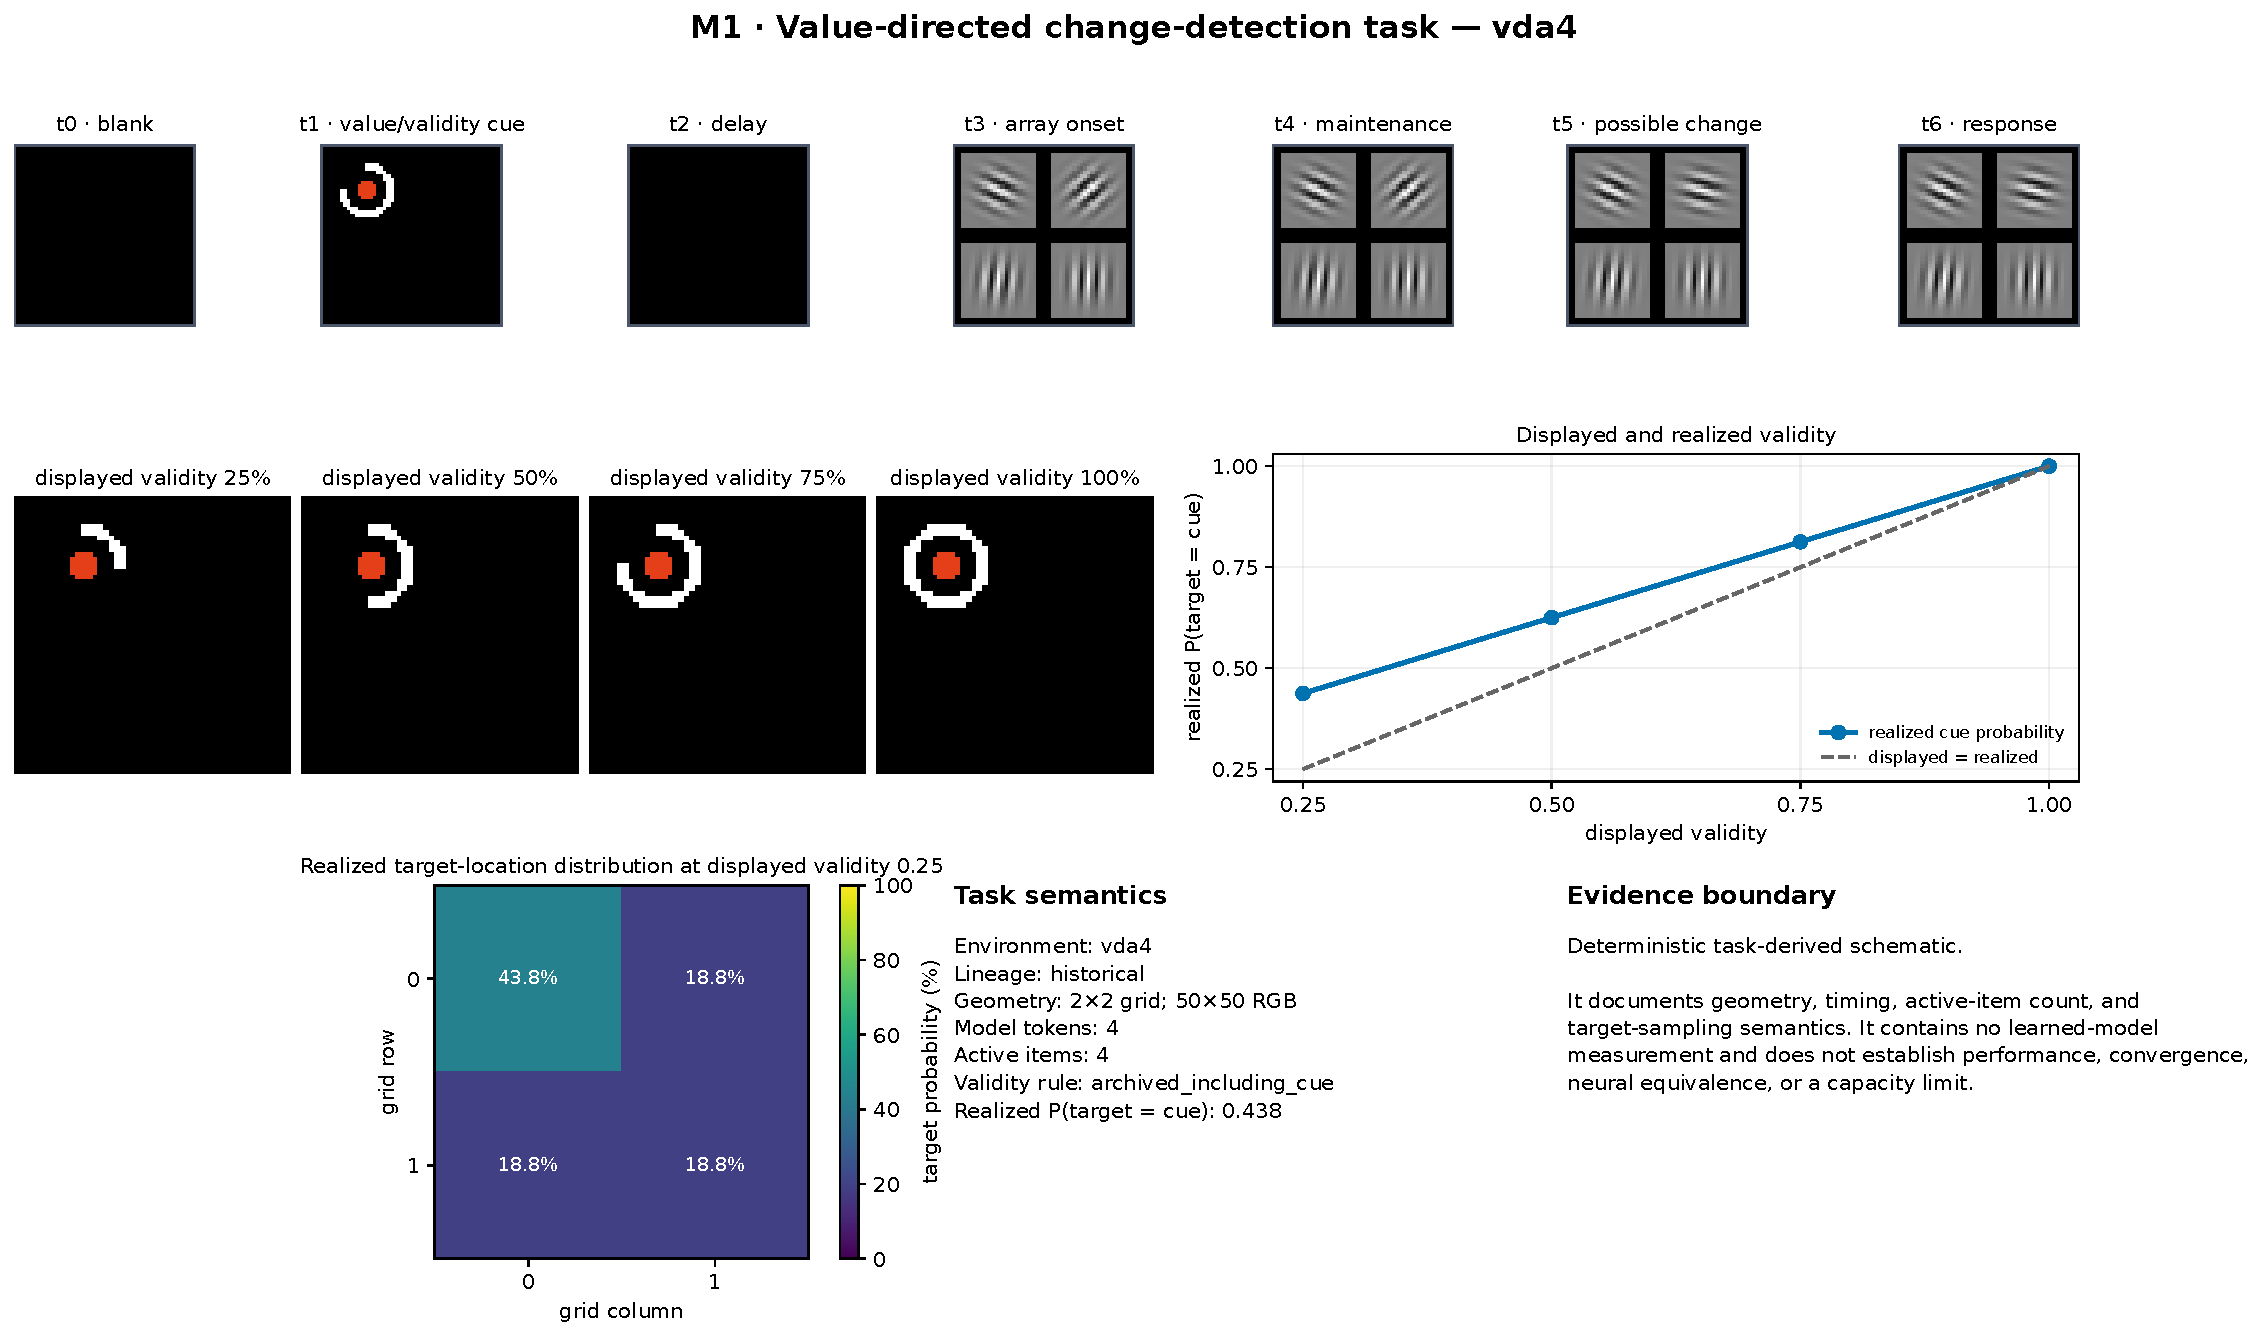
\includegraphics[width=\linewidth]{m1_task_vda4.pdf}
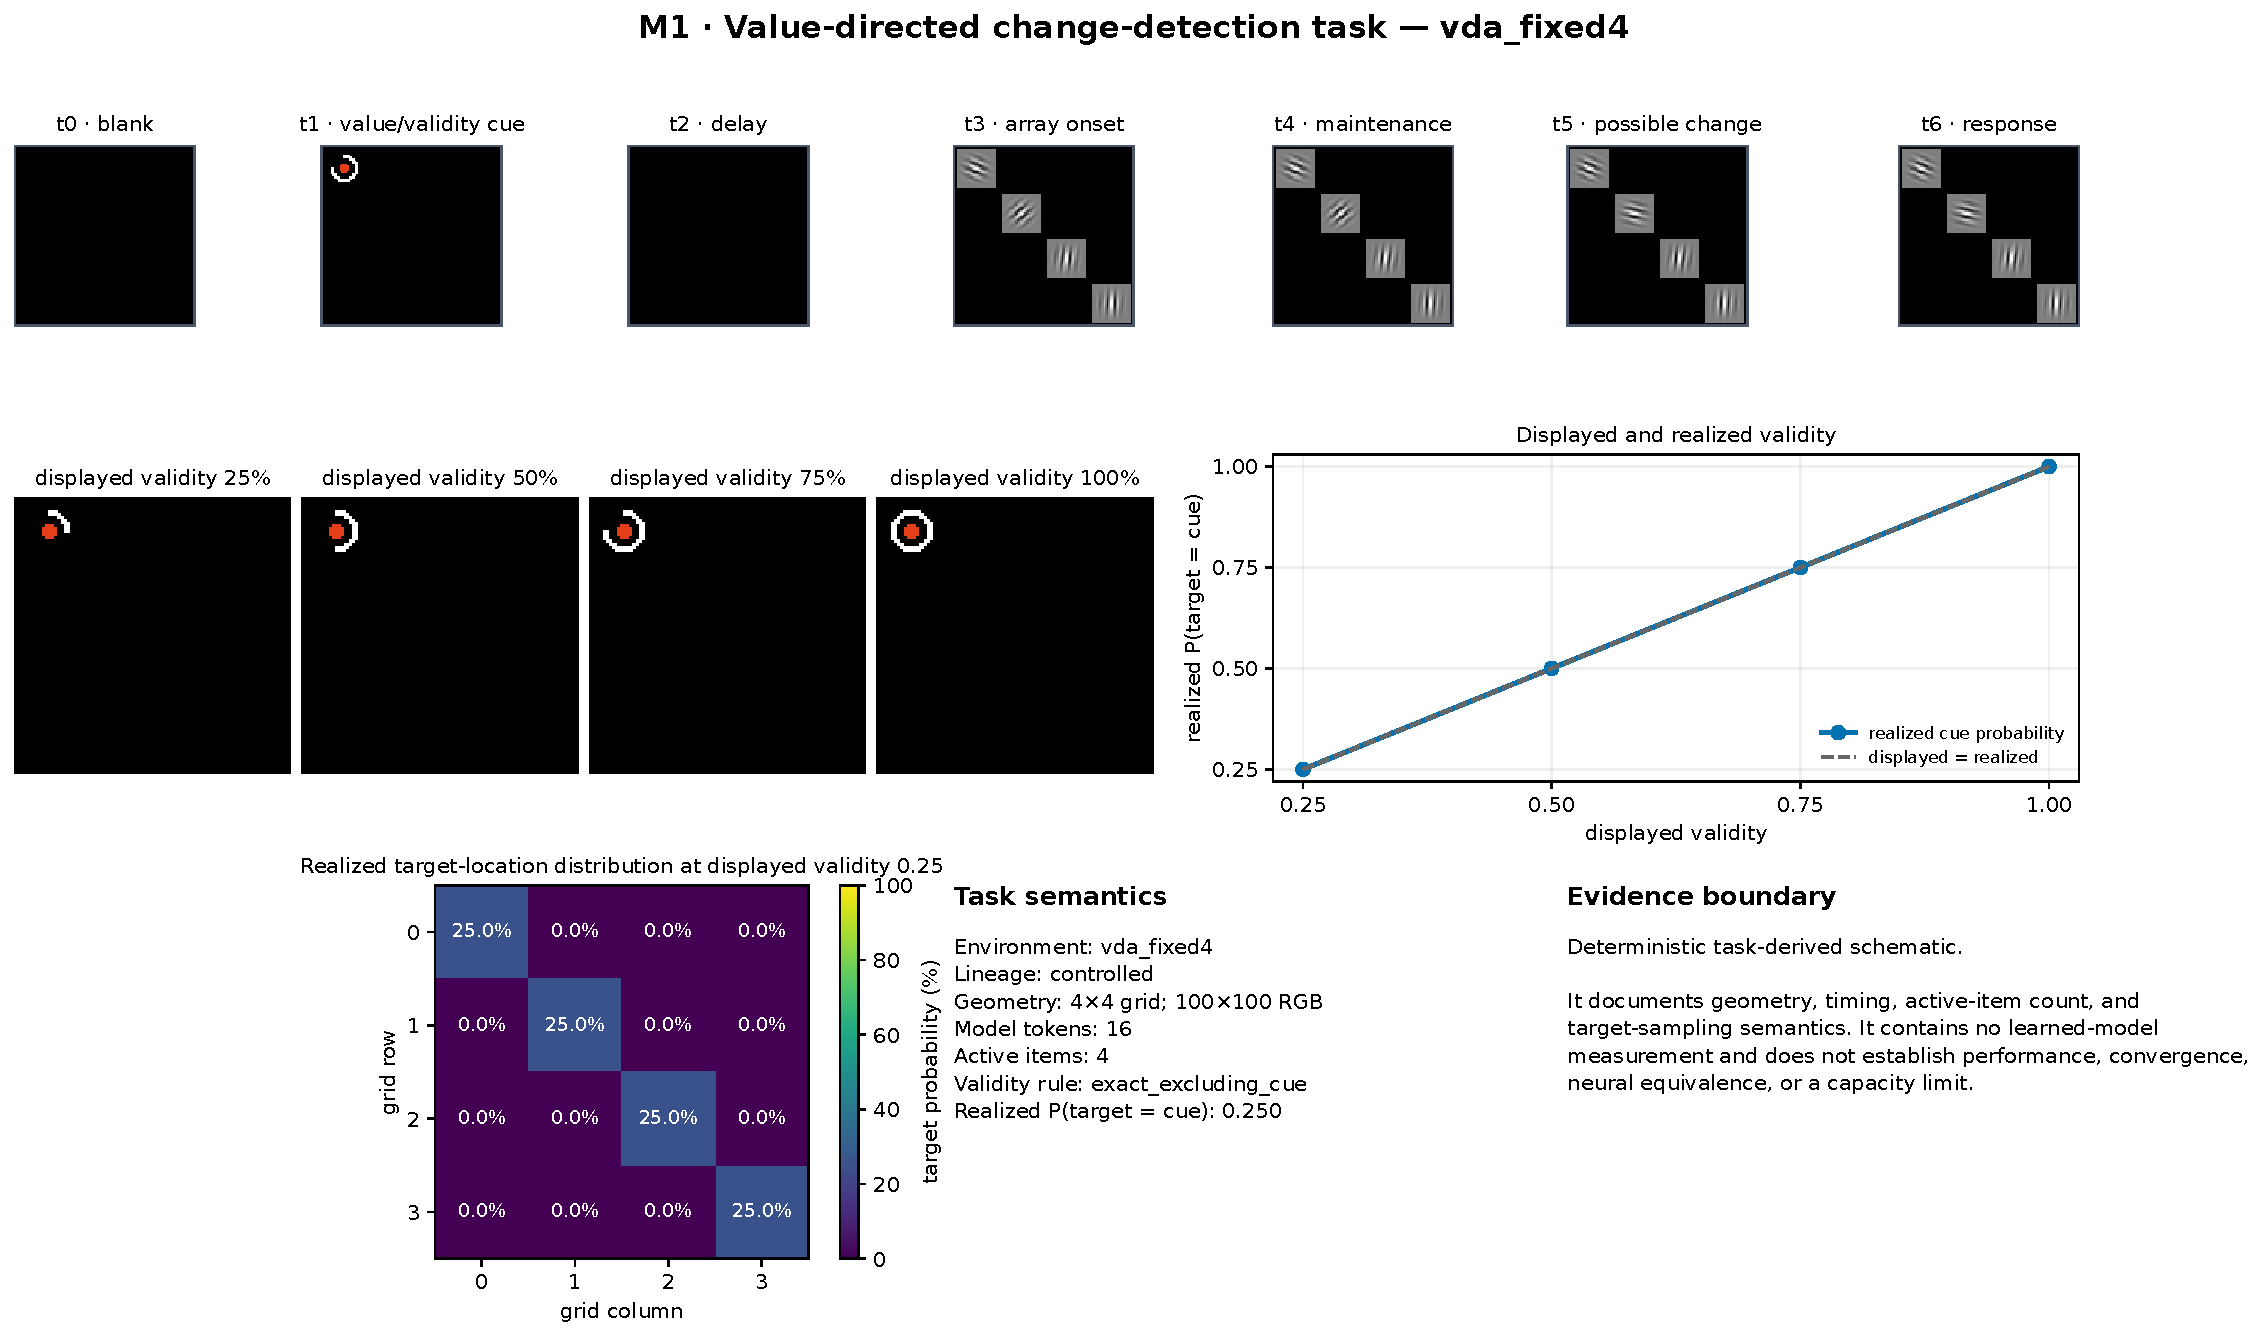
\includegraphics[width=\linewidth]{m1_task_vda_fixed4.pdf}
\caption{\textbf{Historical (top) and controlled fixed-grid (bottom) four-item task specifications.} Deterministic task schematics; seven-frame sequence, geometry, and validity semantics are specified, not measured.}\label{fig:m1-task}
\end{figure}

\subsection{Recurrent architecture}\label{sec:architecture}
The shared pipeline (Figure~\ref{fig:m2-arch}A) converts each frame to spatial patch tokens, routes them through a memory-conditioned attention operator, updates a shared spatial recurrent memory, and reads the flattened state out through actor and critic heads. Two routing families are compared throughout this paper. In \env{affine\_ew} (Figure~\ref{fig:m2-arch}B), memory generates element-wise scale $\gamma$ and shift $\beta$ applied before self-attention, $X'=\gamma\odot X+\beta$. In \env{crossattn1} (Figure~\ref{fig:m2-arch}C), current visual tokens provide queries while visual and recurrent-memory streams jointly provide keys and values, so cross-attention exposes twice as many spatial keys as affine routing for the same token count. Both routers expose the same additive key-logit hook: any attention score can be biased at any chosen spatial key before the softmax, independent of the trial itself. That hook, together with the spatially registered key layout, makes the causal-intervention program in Section~\ref{sec:intervention} possible from $2\times2$ through $10\times10$ native grids.

\begin{figure}[t]
\centering
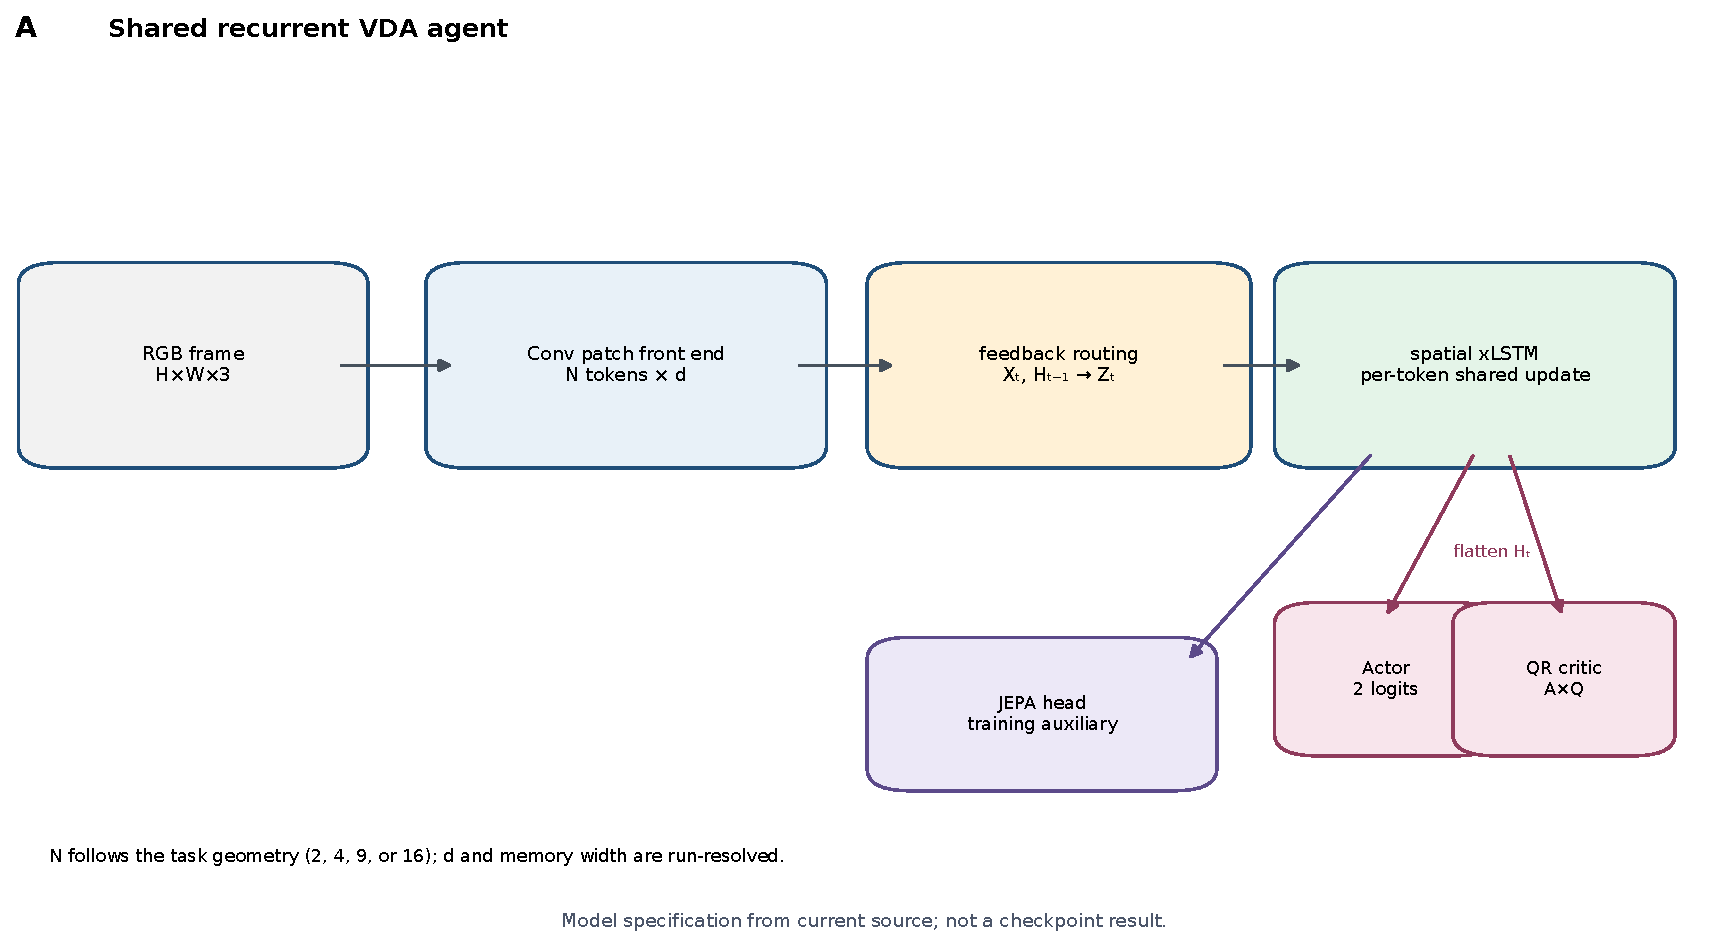
\includegraphics[width=\linewidth]{m2_architecture_a.pdf}\\[2pt]
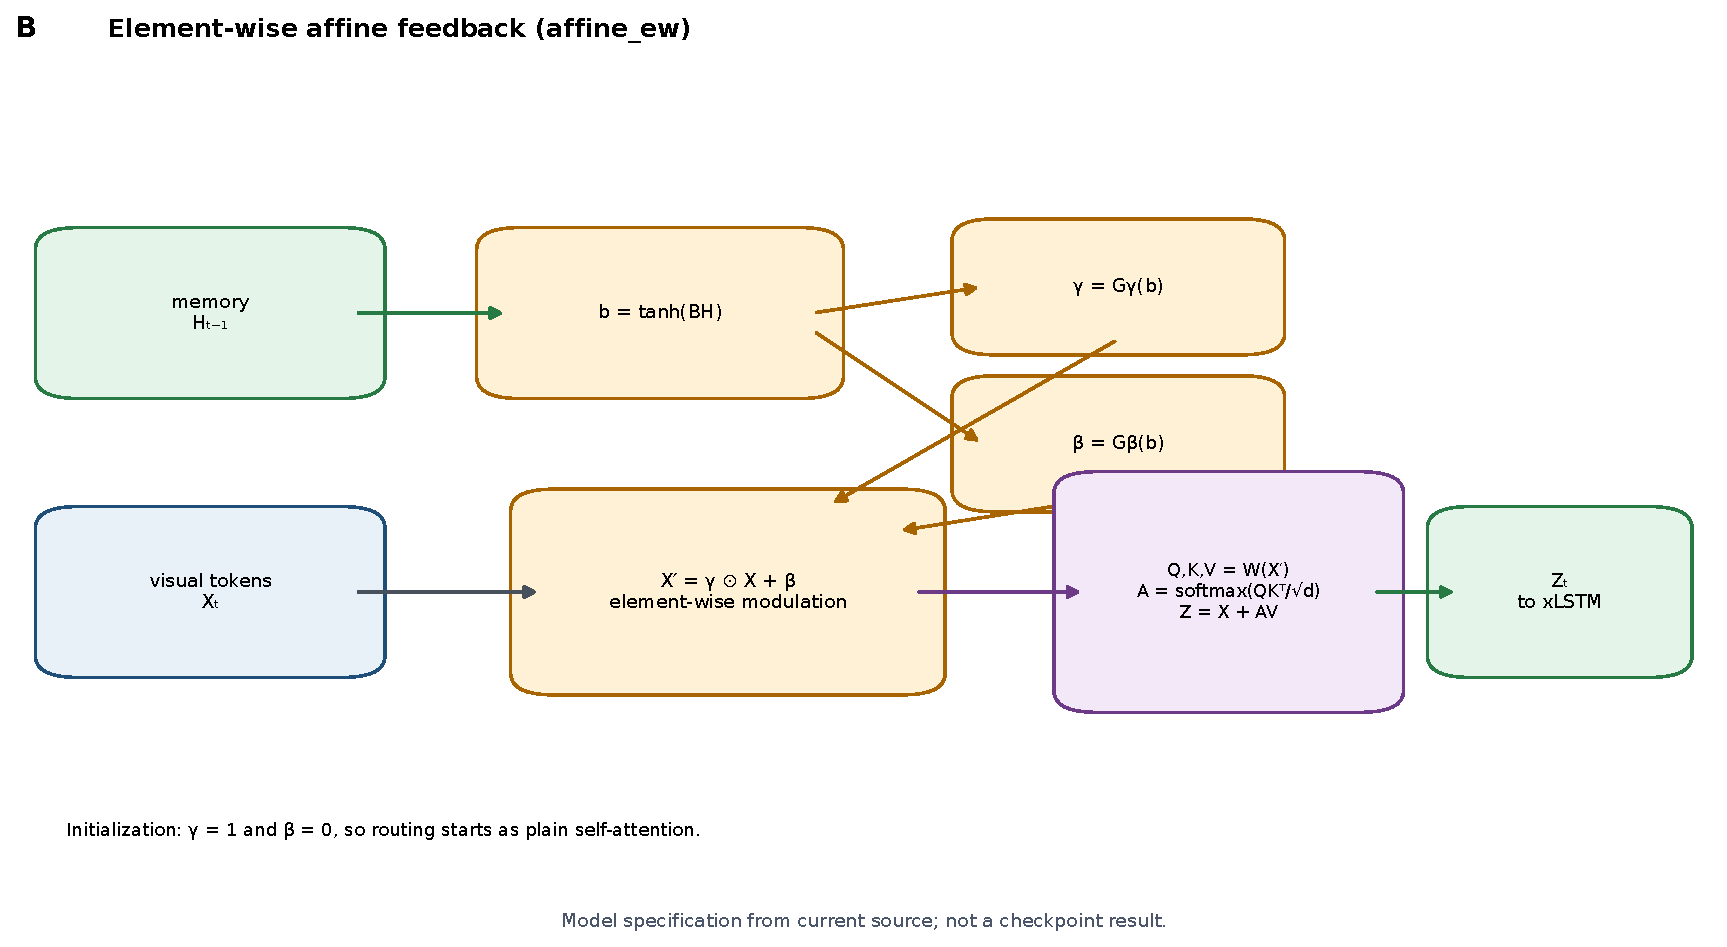
\includegraphics[width=0.49\linewidth]{m2_architecture_b.pdf}\hfill
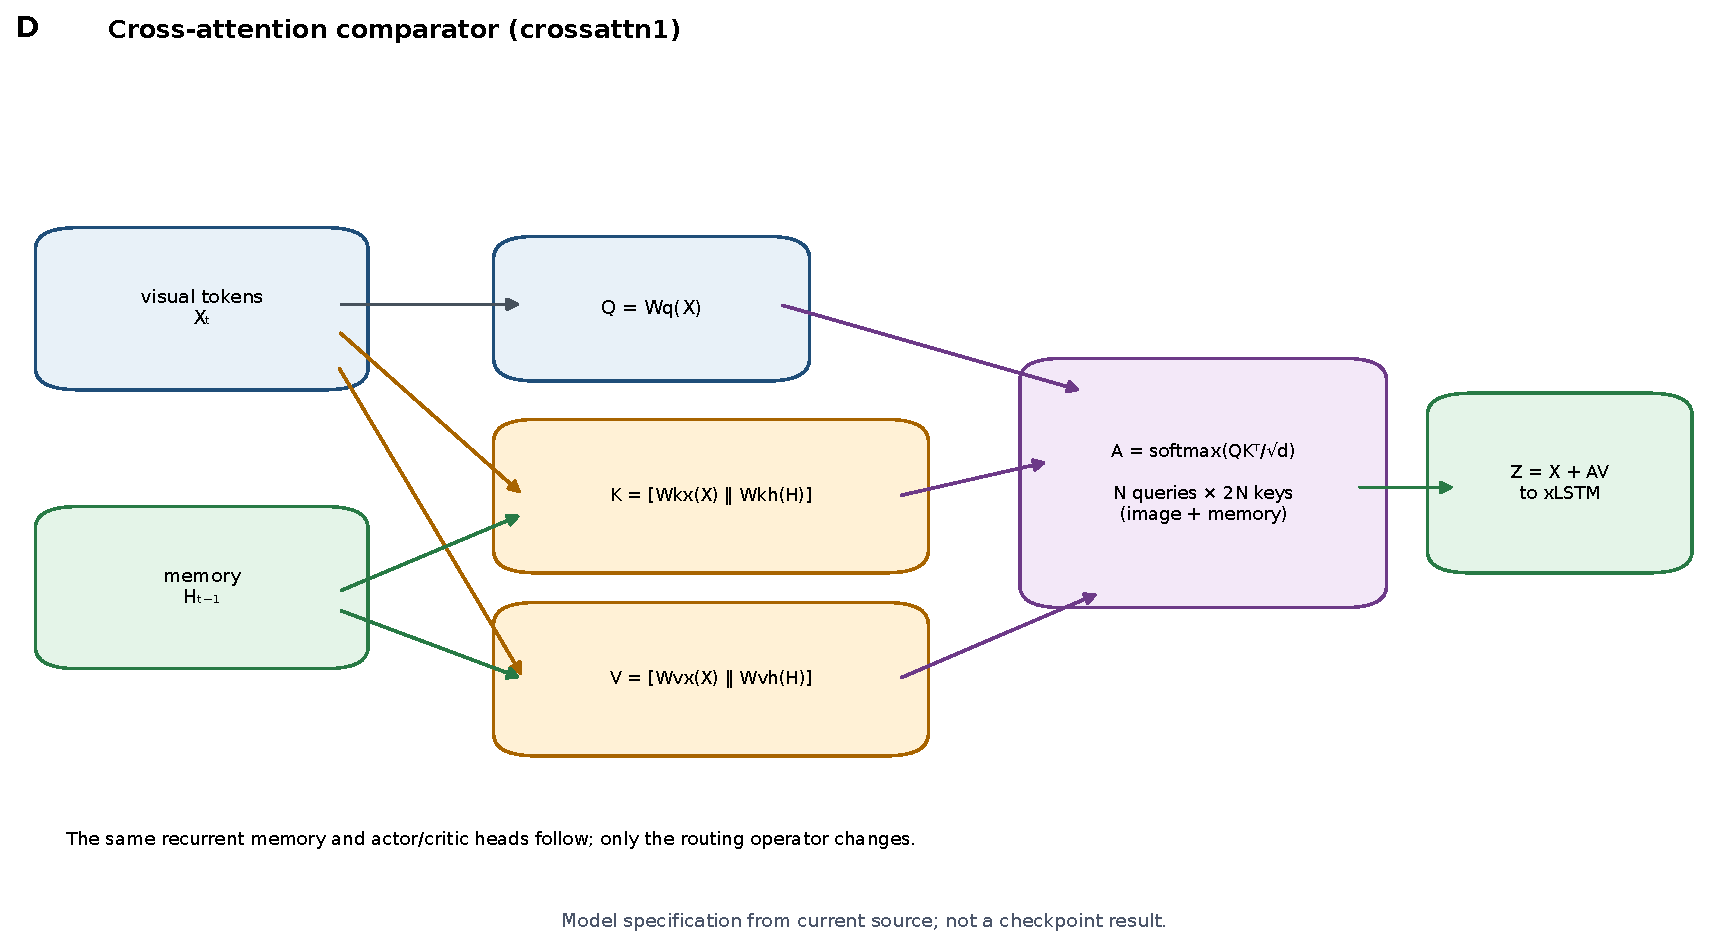
\includegraphics[width=0.49\linewidth]{m2_architecture_d.pdf}
\caption{\textbf{Architecture.} (A) Shared recurrent pipeline: patch tokens, feedback routing, spatial recurrent memory, actor/critic readout. (B) Affine element-wise feedback. (C) Cross-attention feedback: visual queries, visual+memory keys/values. Source-derived specification diagrams, not learned parameter values.}\label{fig:m2-arch}
\end{figure}

\FloatBarrier
\section{Behavioral Signatures}\label{sec:behavior}
This section tests the behavioral tier of the signal-coherence hypothesis with psychometric functions, their discrete-time chronometric counterpart, and signal detection theory wherever a criterion decomposition is available. Carrasco's separation of discriminability from response bias, and Luo and Maunsell's demonstration that a more liberal decision policy can raise hit rate without improving sensory evidence, are the standard we hold every reported cueing effect to \cite{carrasco2011,luo2018}. A larger valid-minus-invalid response gap is evidence for stronger cue dependence, but it is evidence for improved signal coherence only when it is not merely a criterion shift and when representation and causal use agree. We build the case from the broadest, lowest-rigor evidence to the narrowest and most controlled, because claim strength should track evidence strength.

\subsection{A qualitative landscape across the historical ladder}
An aggregate cache spanning set sizes 1, 2, 4, and 9 and both routing families shows the qualitative signature everywhere it can be tested: change-response probability rises and response latency falls with orientation-change magnitude, and, where an uncued comparison is defined, cued responses generally lead uncued ones (Figure~\ref{fig:m3-overview}). \note{This cache carries no producer hash, per-point trial count, or uncertainty interval, and VDA1 has no uncued comparator by construction (a singleton is always cued) -- it establishes a qualitative landscape, not a quantitative one.}

\begin{figure}[t]
\centering
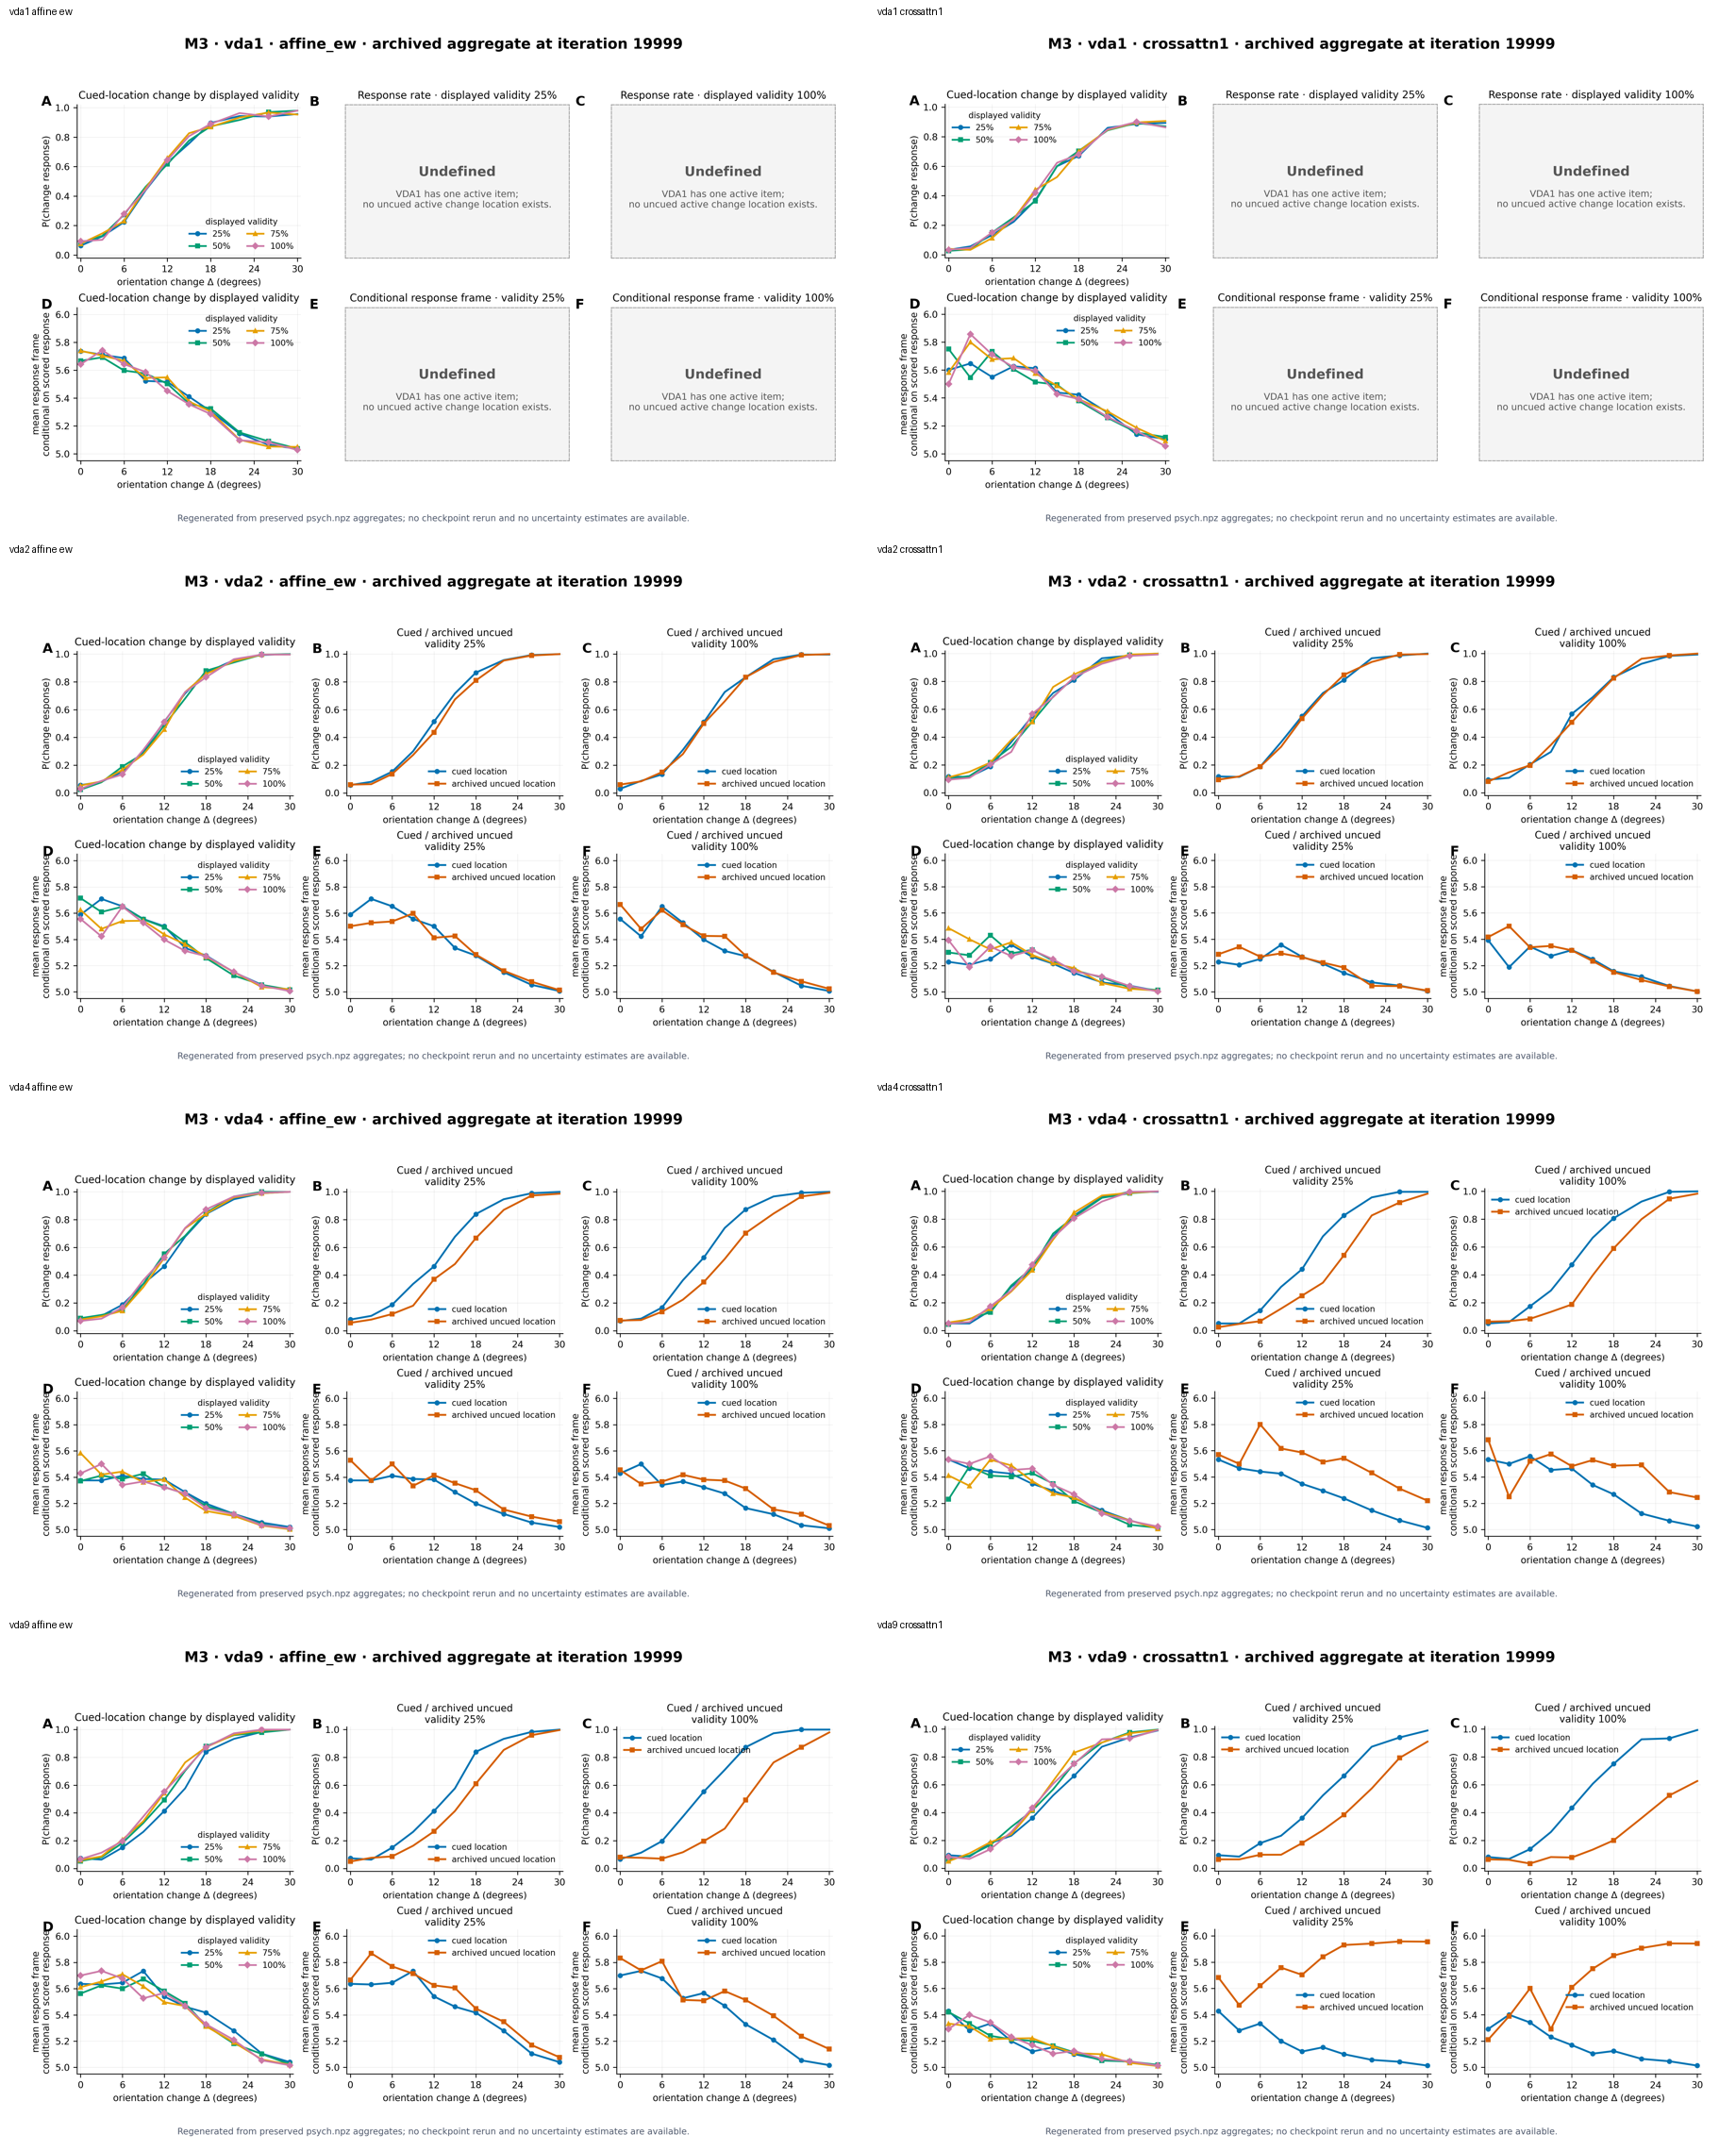
\includegraphics[width=\linewidth]{m3_behavior_contact_sheet.png}
\caption{\textbf{Cueing looks behaviorally real across the historical ladder.} Rows: VDA1, VDA2, VDA4, VDA9; columns: affine then cross-attention. A--C response probability, D--F conditional response frame. Regenerated from a preserved aggregate archive; checkpoints not rerun.}\label{fig:m3-overview}
\end{figure}

\subsection{Checkpoint-verified psychometrics at set sizes 4 and 9}\label{sec:first-wave-behavior}
A separate, provenance-closed recomputation executes one iteration-19{,}999 checkpoint per task--routing pair directly (VDA4 and VDA9, both routing families), fixing the cue at S1 and sweeping displayed cue proportion while forcing the change to the cued location or a fixed opposite location (S4 or S9). Three hundred trials back every point. Change-response probability rises with orientation change in every checkpoint, and fixed-cued estimates exceed fixed-opposite estimates at intermediate magnitudes (Figure~\ref{fig:first-wave-psych}).

\begin{figure*}[t]
\centering
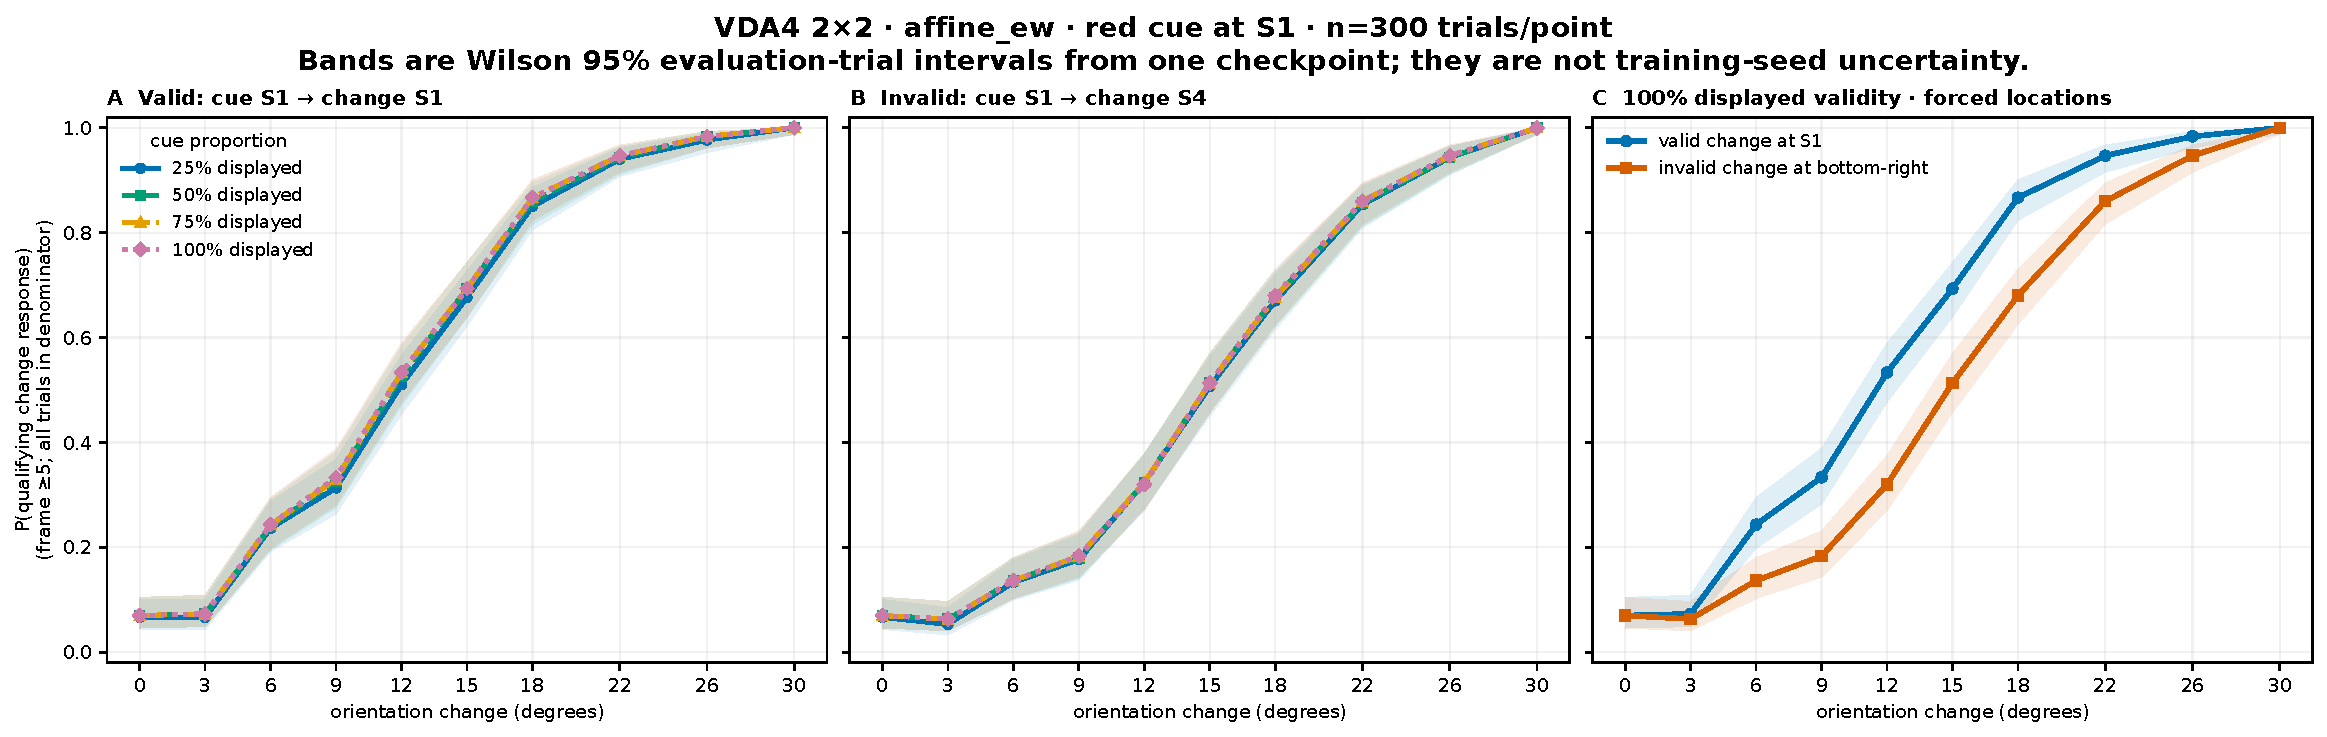
\includegraphics[width=0.49\textwidth]{first_wave_psychometric_vda4_affine_ew.pdf}\hfill
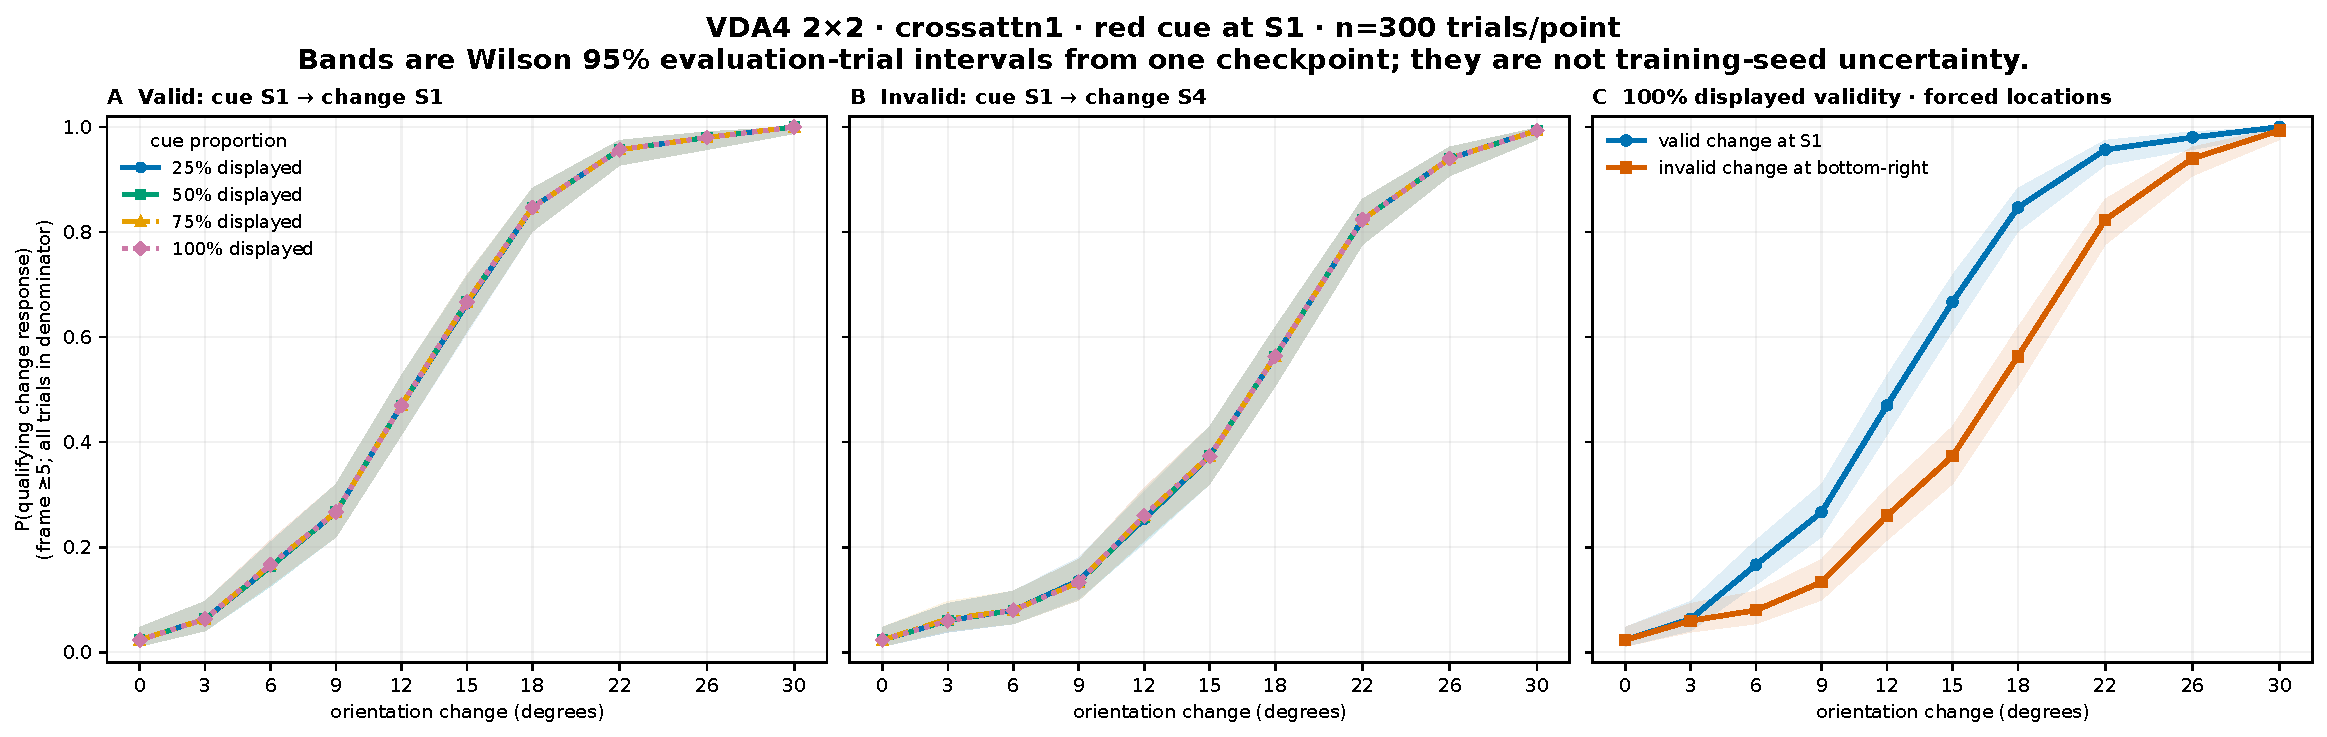
\includegraphics[width=0.49\textwidth]{first_wave_psychometric_vda4_crossattn1.pdf}\\[4pt]
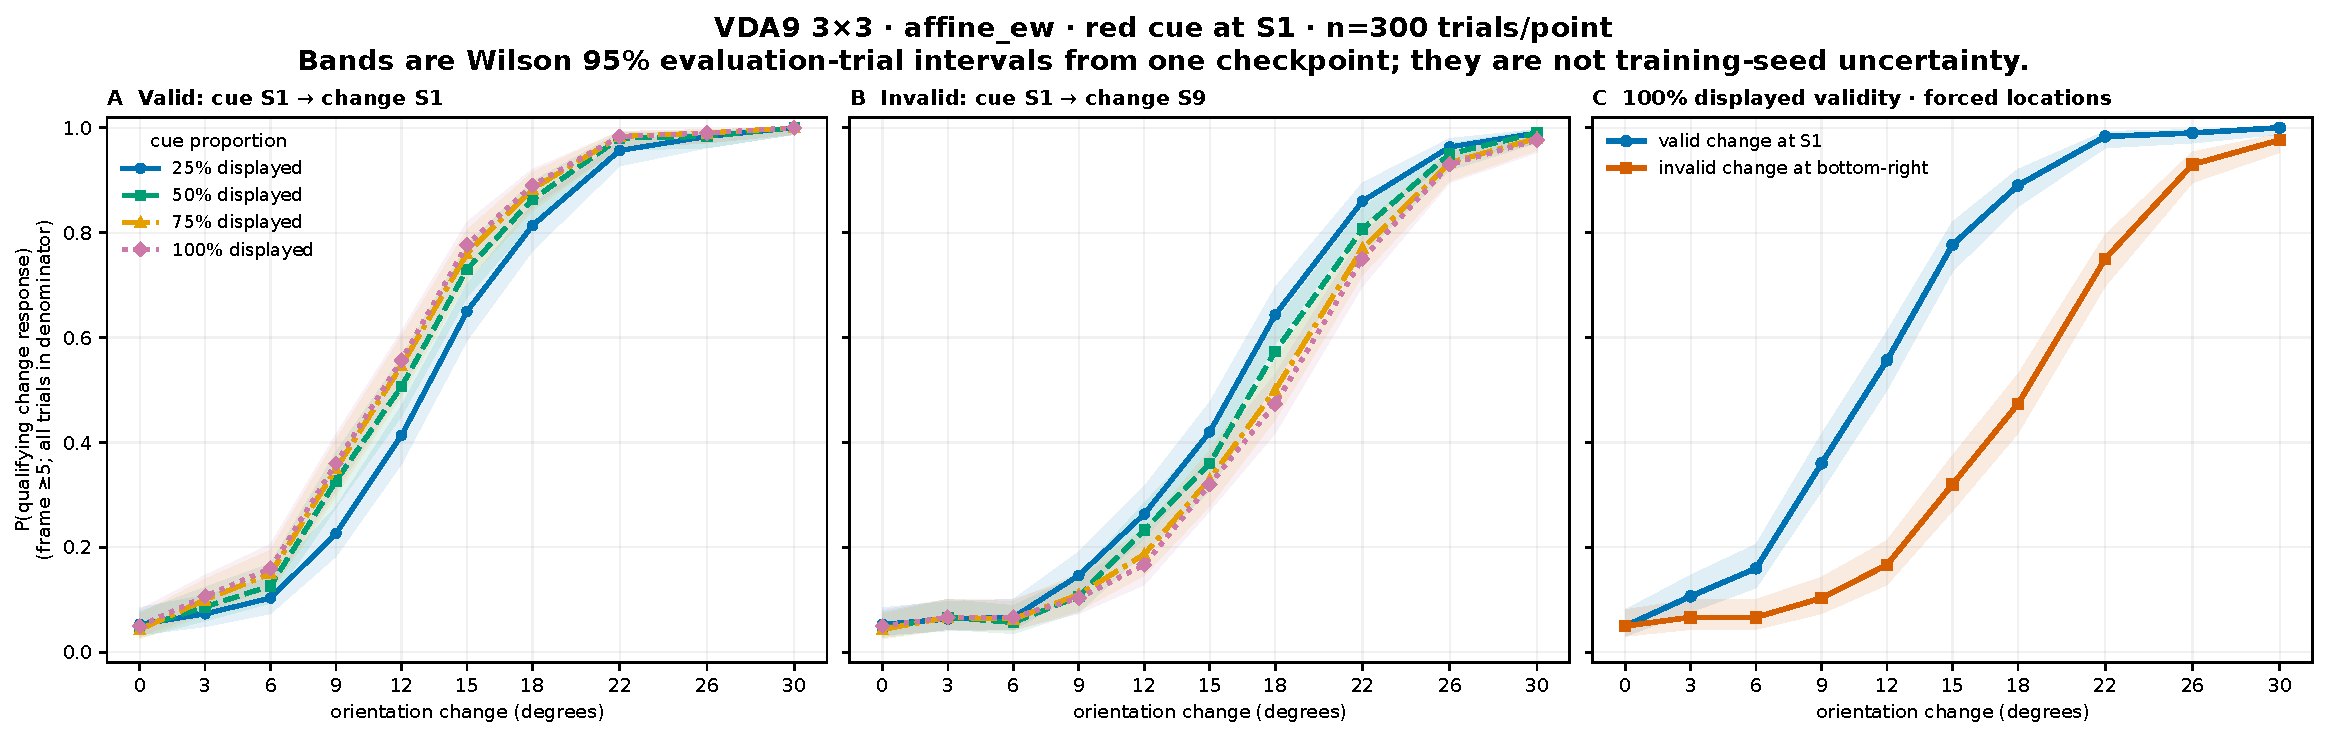
\includegraphics[width=0.49\textwidth]{first_wave_psychometric_vda9_affine_ew.pdf}\hfill
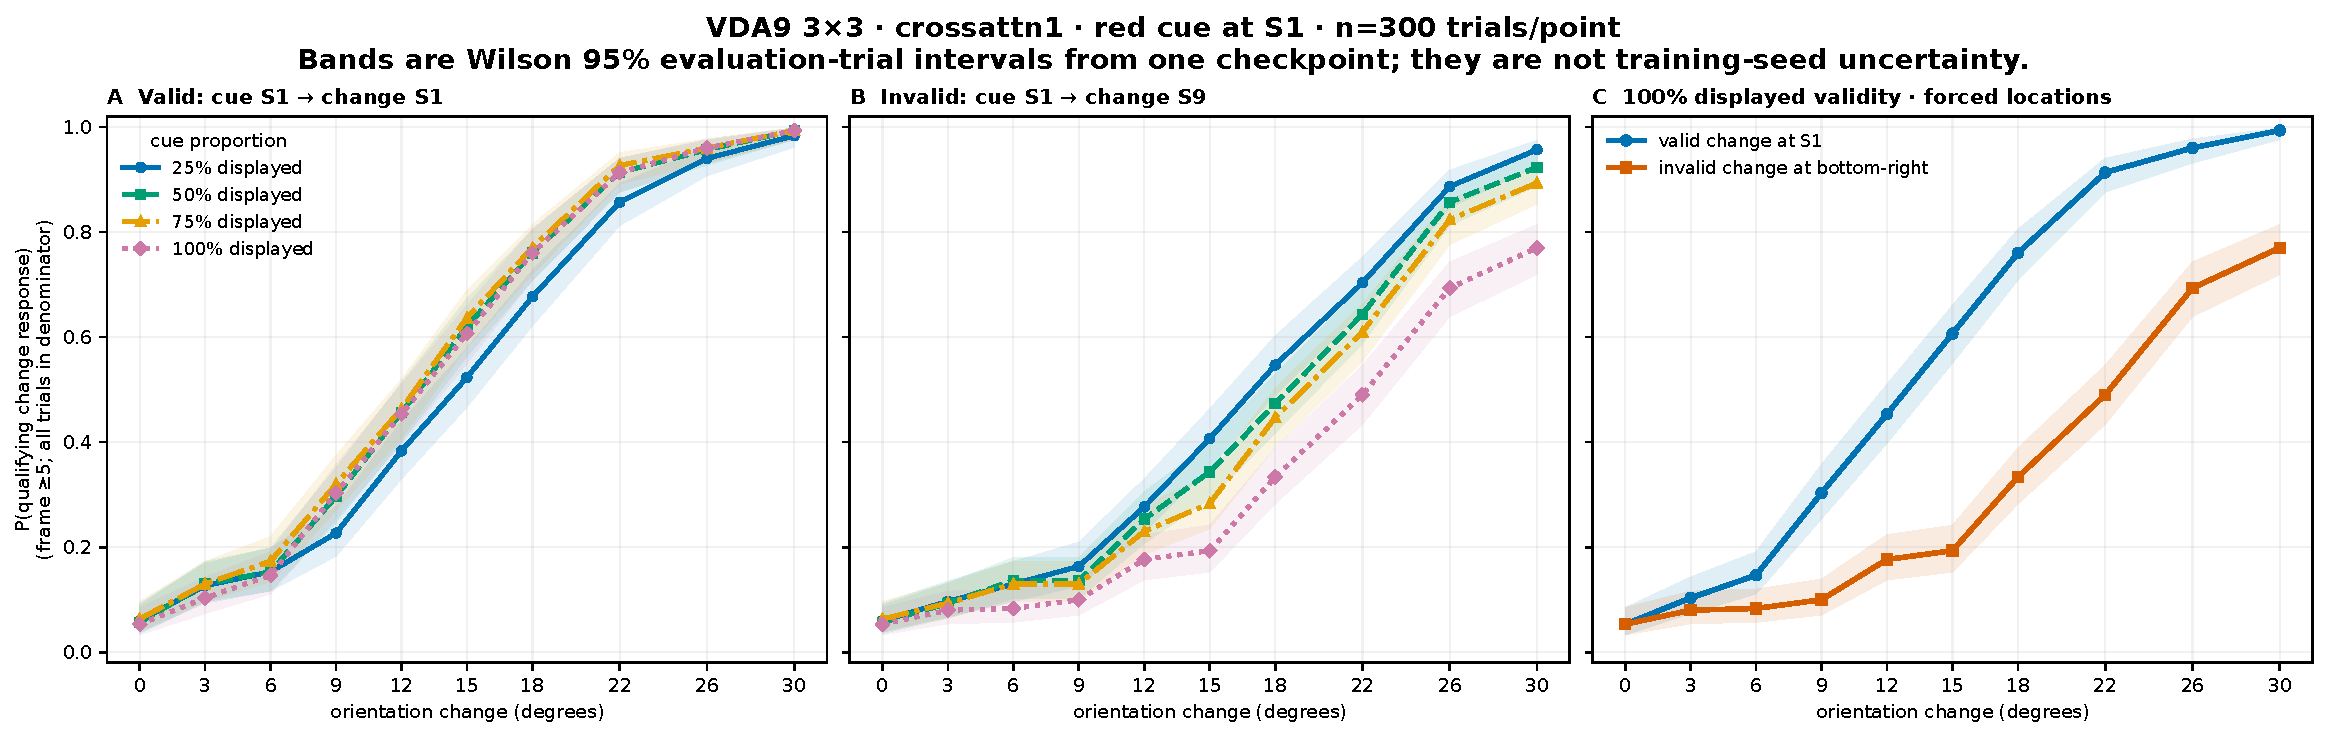
\includegraphics[width=0.49\textwidth]{first_wave_psychometric_vda9_crossattn1.pdf}
\caption{\textbf{Checkpoint-recomputed psychometrics, 300 trials/point, Wilson 95\% intervals.} Top: VDA4, affine (left) and cross-attention (right). Bottom: VDA9. Panels A/B fix the change at the cued or opposite location while sweeping displayed cue proportion; Panel C re-plots their 100\%-displayed endpoints.}\label{fig:first-wave-psych}
\end{figure*}

\subsection{Does recurrent width change the cueing benefit?}\label{sec:width-behavior}
A matched battery pairs each first-wave checkpoint (plus VDA1) with a separately trained checkpoint carrying twice the recurrent width ($d_\mathrm{mem}=256$ vs.\ 128). Width here is a descriptive grouping contrast, not a causal manipulation -- the paired checkpoints were trained separately. At $14^\circ$, VDA1 cross-attention gains 21 percentage points going from d128 to d256, while VDA4 cross-attention \emph{loses} 13; none of the five admitted pairs share a common direction (Figure~\ref{fig:matched-width}A). \textbf{A wider recurrent state does not consistently produce a larger cueing benefit}, foreshadowing the routing-family result of Section~\ref{sec:psychometric-fits}: capacity-like manipulations of this architecture do not behave like a clean capacity law.

\begin{figure*}[t]
\centering
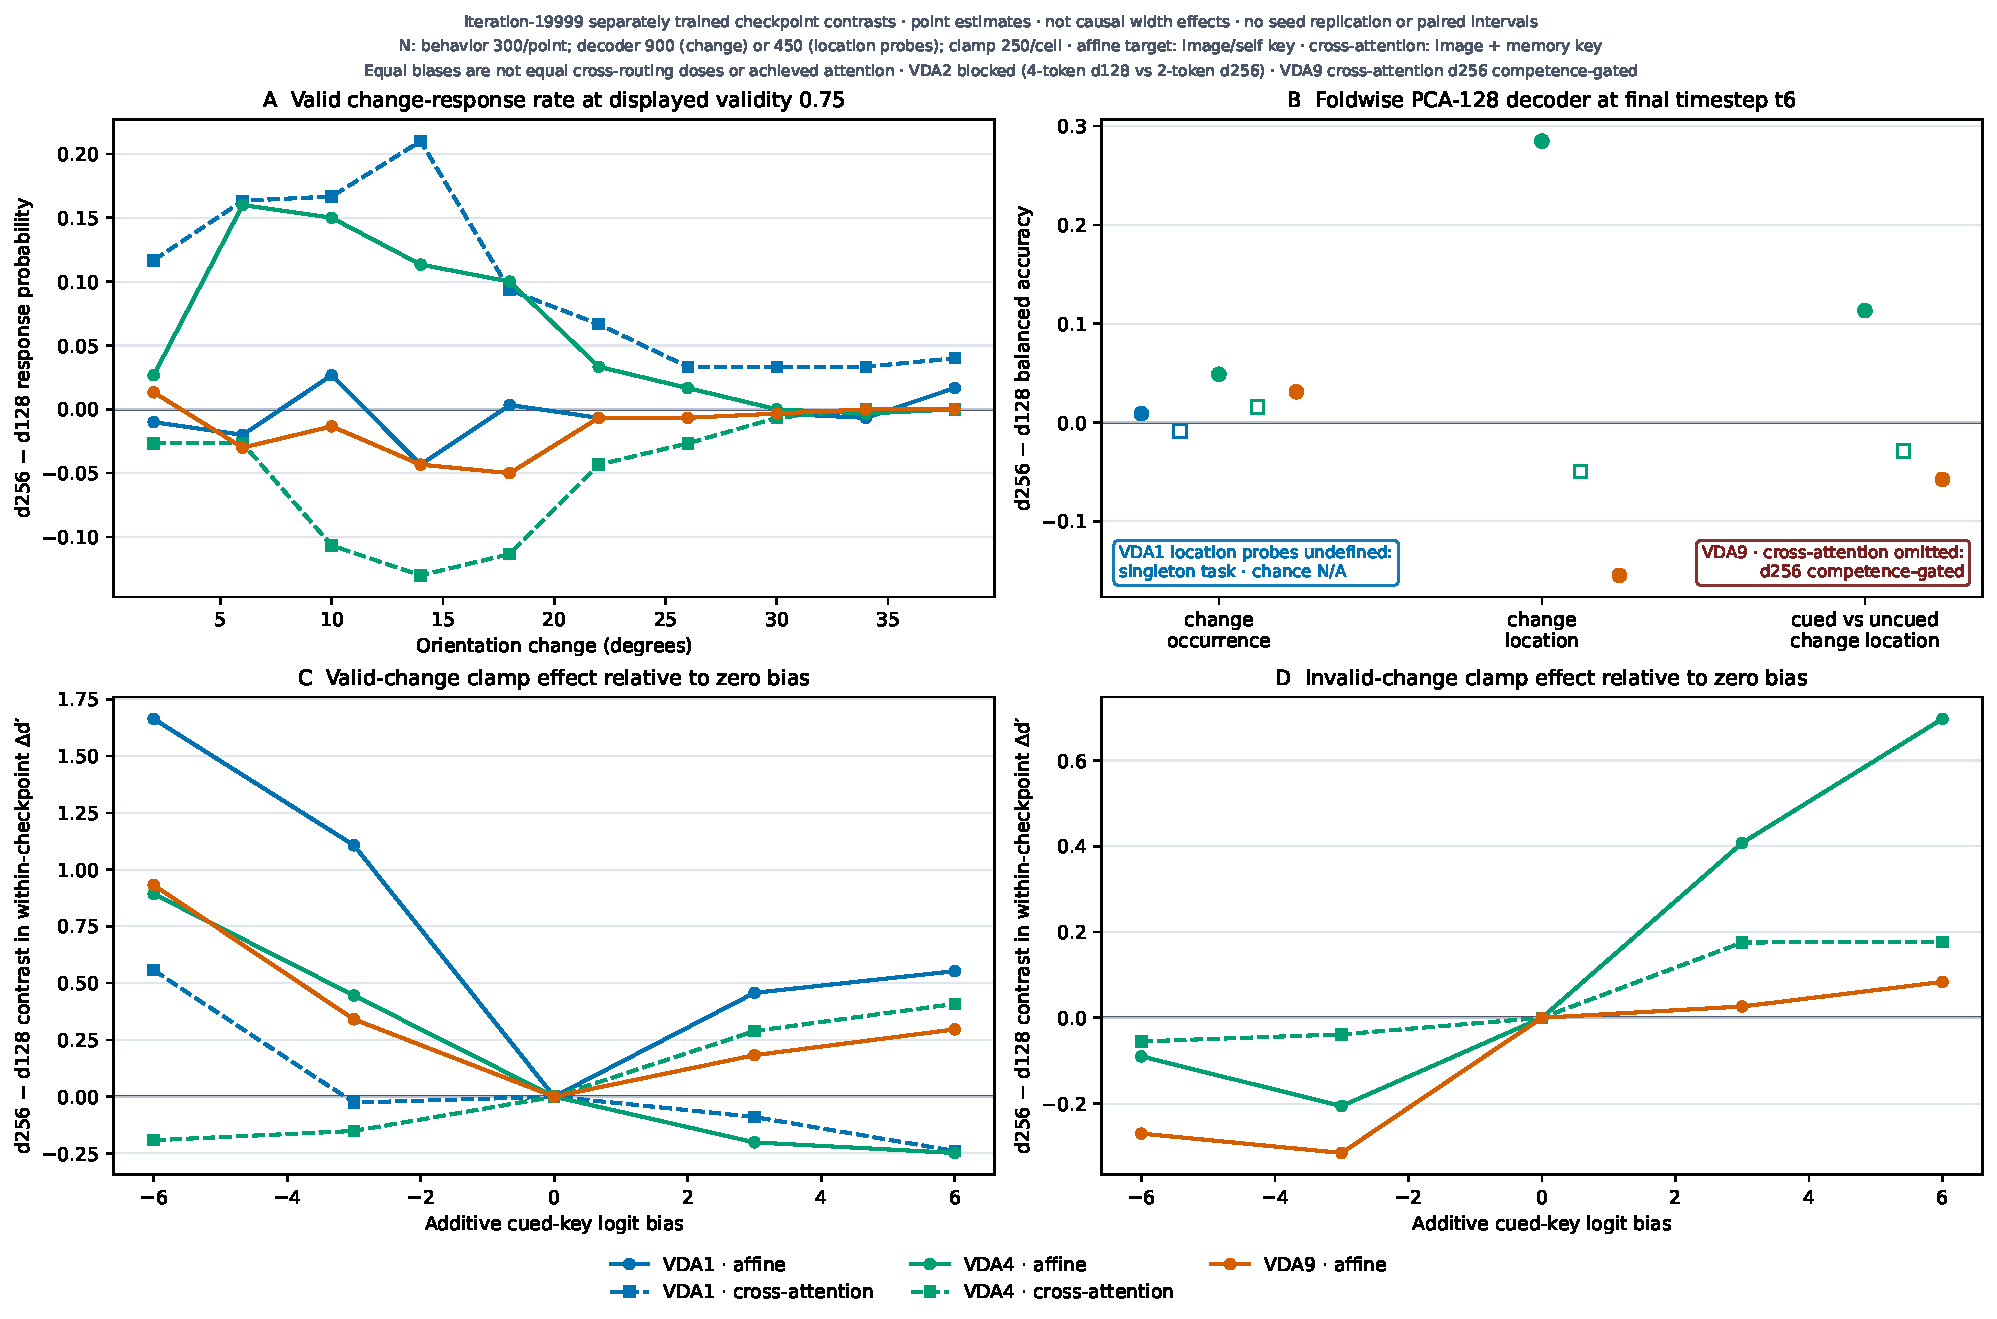
\includegraphics[width=0.85\textwidth]{matched_width_summary.pdf}
\caption{\textbf{Width does not predict the cueing benefit.} Five d256-vs-d128 checkpoint pairs, no consistent direction. (A) Valid-location response differences (behavioral). (B) t6 decoder differences (Section~\ref{sec:width-decoding}). (C--D) Within-checkpoint $d'$ change from an additive routing-key bias, compared across width (Section~\ref{sec:existing-intervention}).}\label{fig:matched-width}
\end{figure*}

\subsection{VDA16: large cueing contrasts in two controlled $K=16$ checkpoints}\label{sec:vda16-behavior}
Two controlled VDA16 checkpoints -- fixed $4\times4$ grid, sixteen tokens, $d_\mathrm{mem}=128$, seed 0, one cross-attention and one affine -- reached terminal iteration 19{,}999 and passed the VDA16 production validation gate. Neither reached the task's declared $8^\circ$ curriculum floor (cross-attention plateaued at $\theta=65^\circ$, affine advanced further to $\theta=47^\circ$ after a statefully resumed training run), so both are \emph{competence-gated} diagnostics of an easy condition rather than evidence of full convergence.

At displayed validity 0.75 and the change nearest $18^\circ$, cross-attention's qualifying response rate is \textbf{0.653 valid vs.\ 0.133 forced-invalid} ($\Delta=+0.520$); a second, independent rerun with a 100\%-valid cue and the change forced to the cued location or the opposite corner reproduces the pattern at an unambiguous ceiling: \textbf{0.983 vs.\ 0.490} at $30^\circ$ (conditional mean response frames 5.20 vs.\ 5.96). The affine checkpoint shows the same qualitative pattern with a smaller gap at the same probe -- \textbf{0.893 vs.\ 0.480} ($\Delta=+0.413$) -- but stronger final-timestep decodability of change occurrence, realized location, and cued-vs-uncued location than its cross-attention counterpart (Figure~\ref{fig:vda16-behavior}). The eight-curve overlays in Figure~\ref{fig:vda16-overlay} make the routing-family contrast vivid: affine's valid and forced-invalid curves are nearly coincident across displayed cue proportions 25--75\%, diverging only at the 100\%-displayed, fully out-of-policy stress test, whereas cross-attention shows a graded, pronounced cue-proportion dependence throughout. \note{These are separately trained, single-seed checkpoints with different achieved curricula; the routing-family contrast is descriptive.}

\begin{figure*}[t]
\centering

\includegraphics[width=0.49\textwidth]{vda16_manuscript_summary.pdf}\hfill
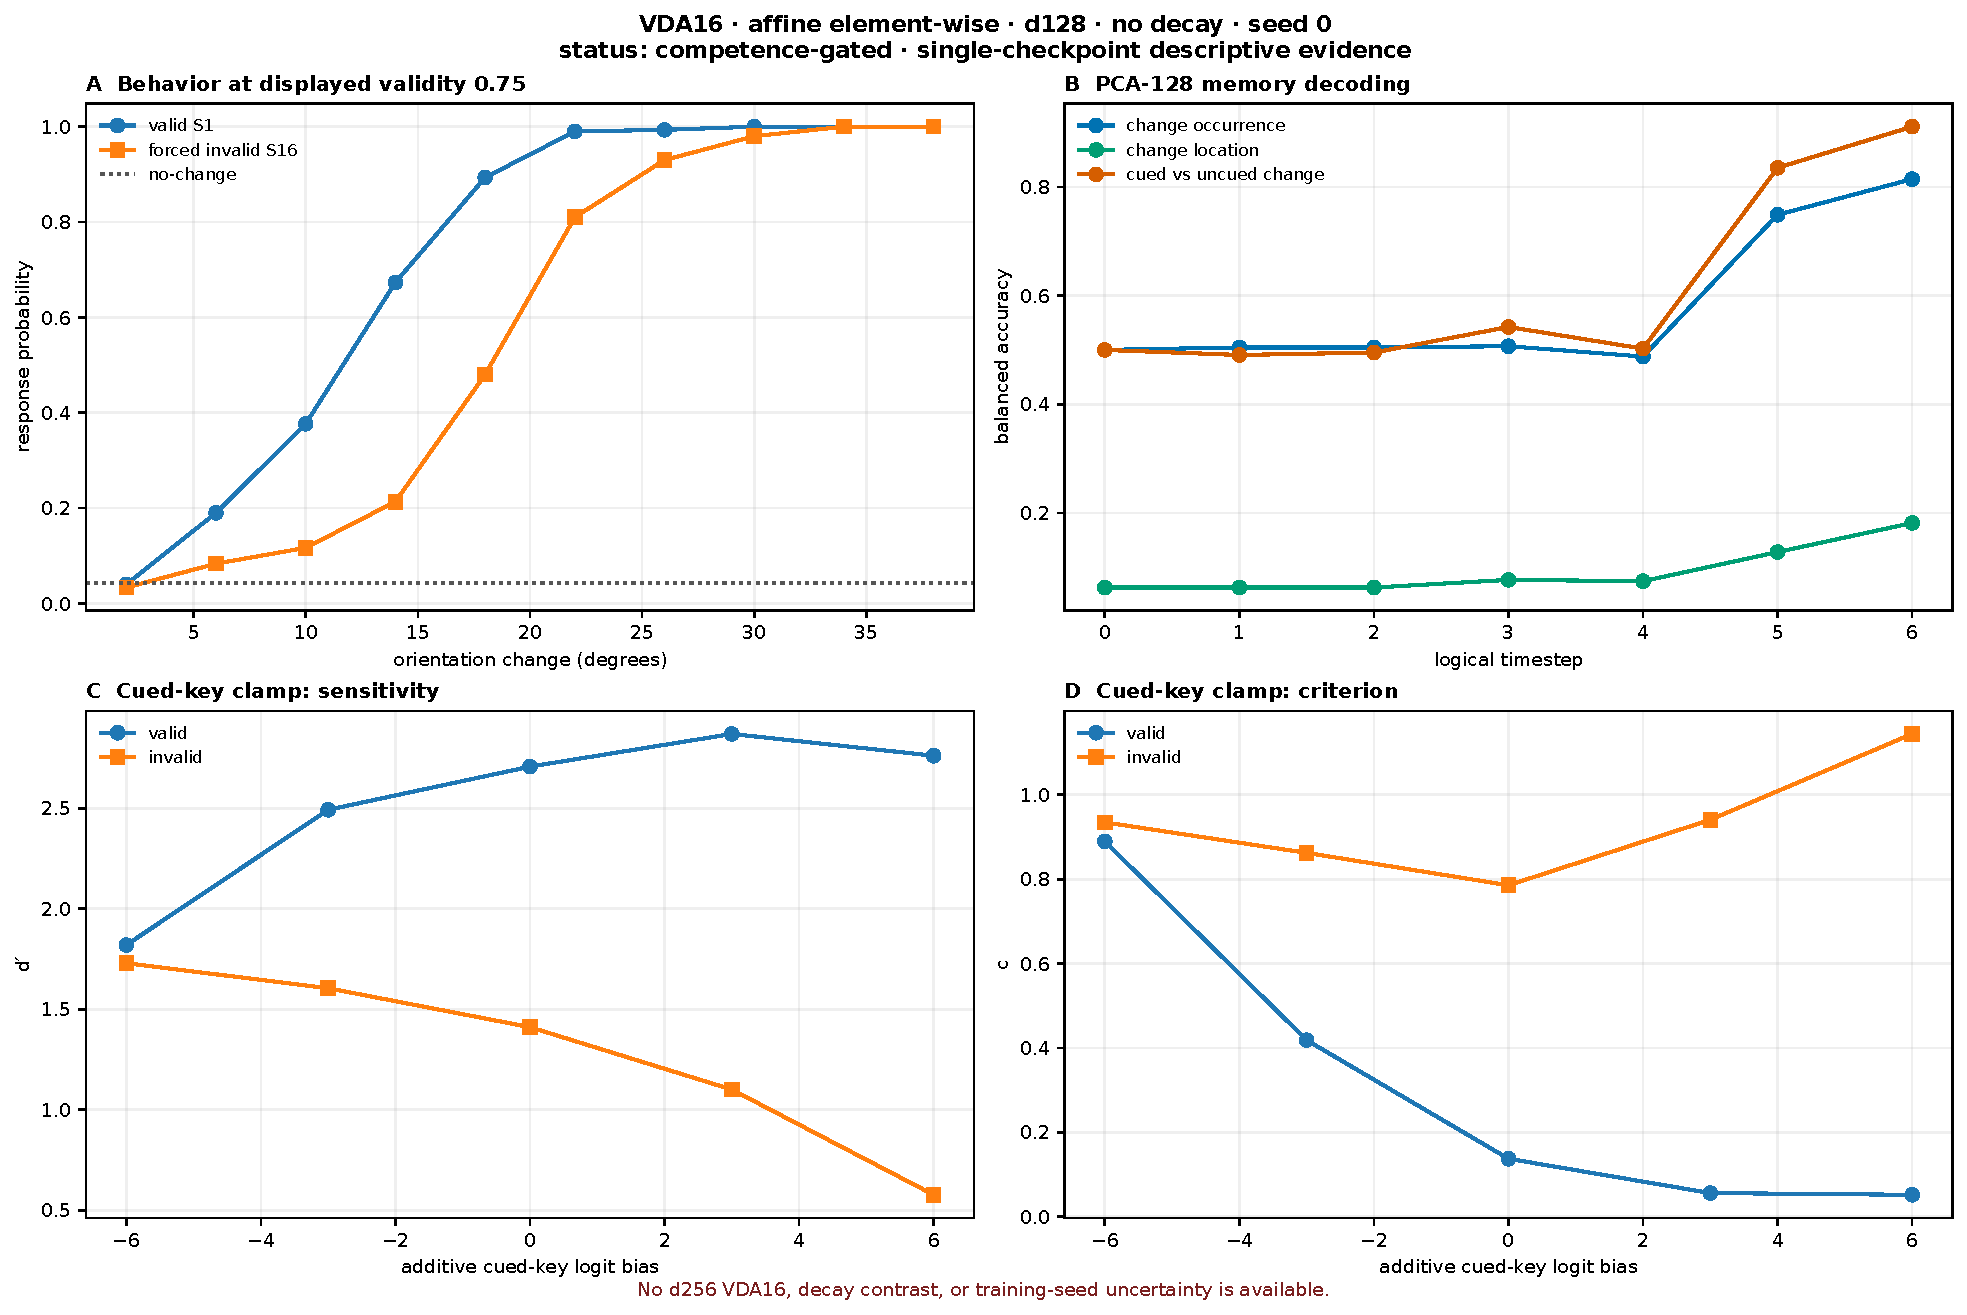
\includegraphics[width=0.49\textwidth]{vda16_affine_manuscript_summary.pdf}
\caption{\textbf{VDA16 cross-attention (left) and affine (right).} (A) Matched-bank response rates. (B) Foldwise PCA-128 decoding. (C--D) Sensitivity/criterion under additive cued-key bias (Section~\ref{sec:existing-intervention}). Both checkpoints reached iteration 19{,}999 but remain competence-gated; d256, decay-contrast, and replicated-seed cells are not admitted.}\label{fig:vda16-behavior}
\end{figure*}

\begin{figure*}[t]
\centering
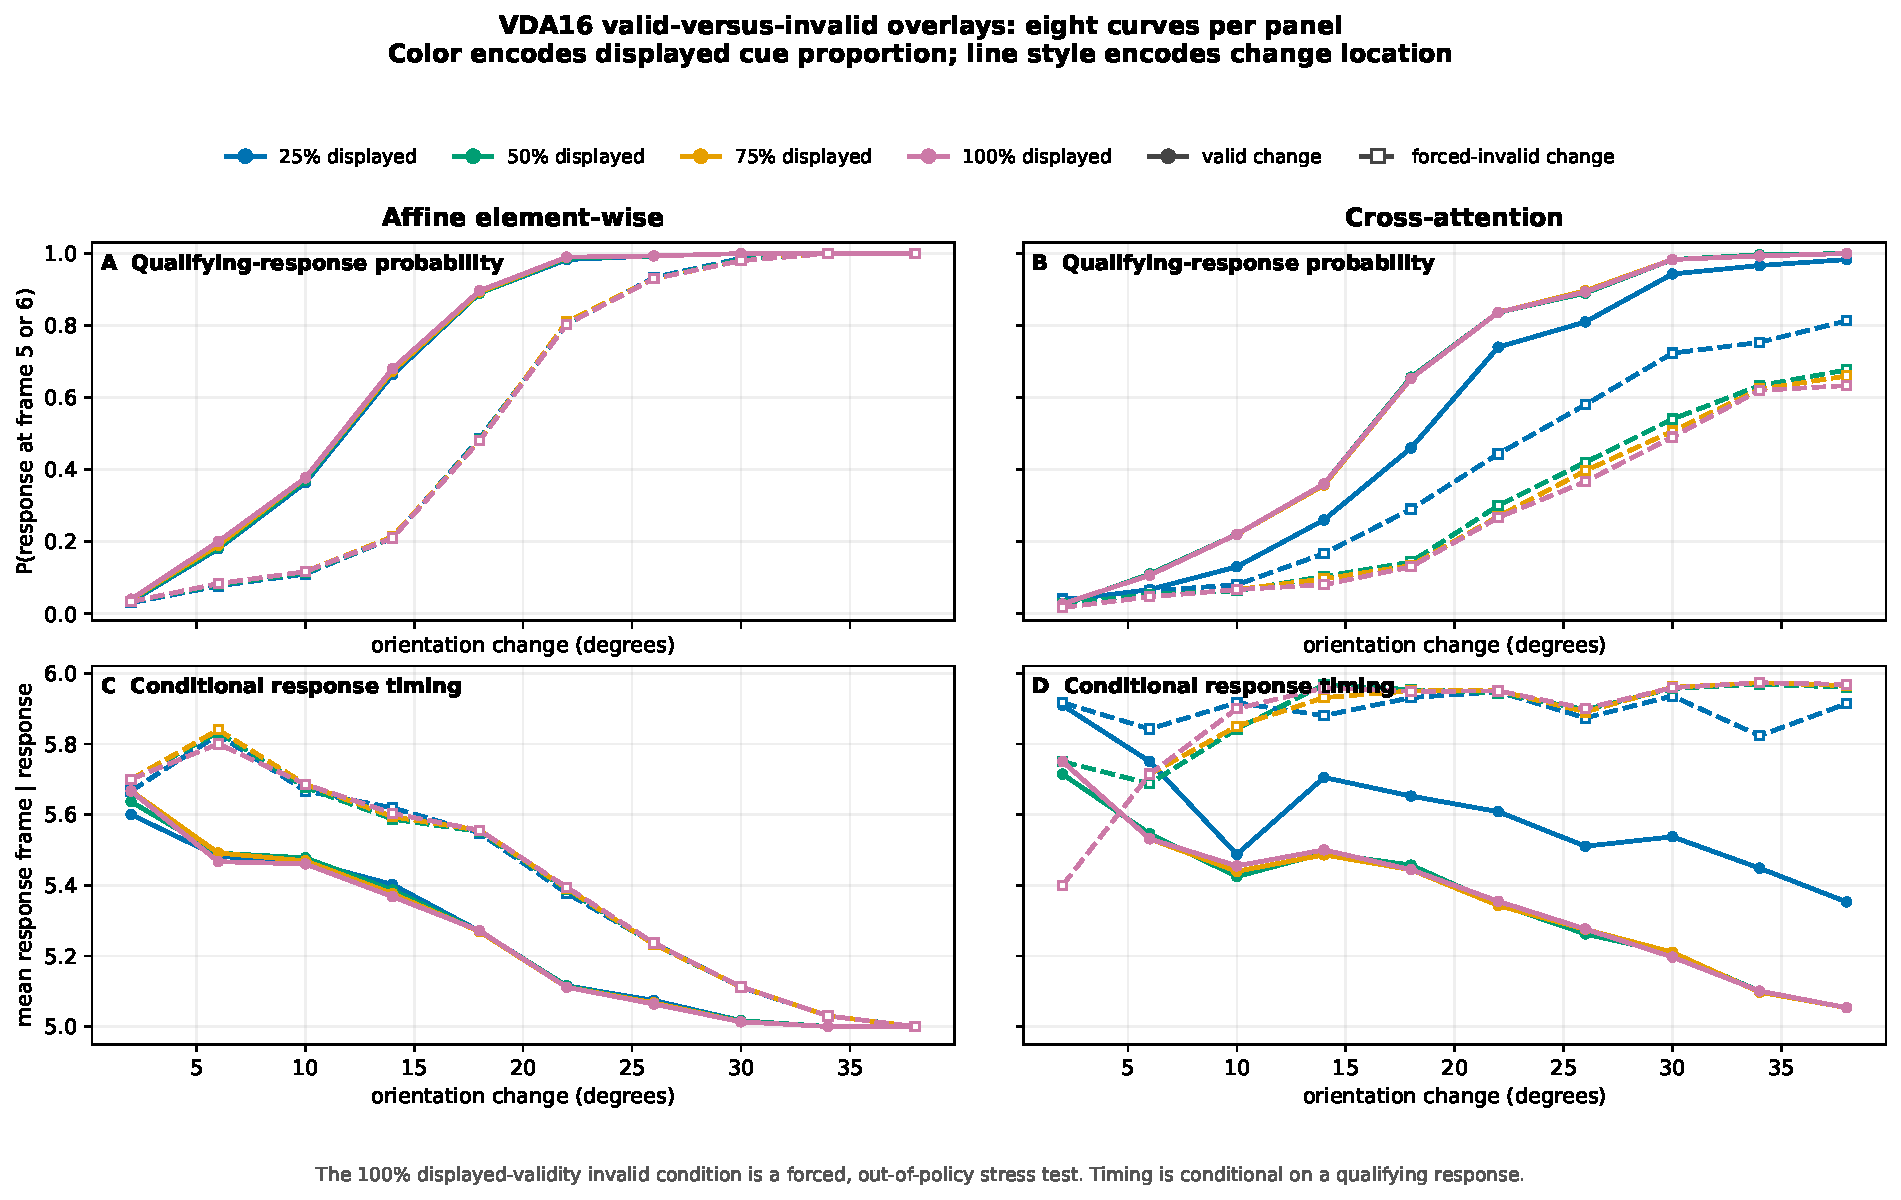
\includegraphics[width=0.85\textwidth]{vda16_valid_invalid_eight_curve_overlay.pdf}
\caption{\textbf{Affine's valid/invalid curves barely separate below 100\% displayed validity; cross-attention's separate throughout.} Four displayed cue proportions overlaid per panel, valid changes at S1 (solid) vs.\ forced-invalid changes at S16 (dashed). Top: response probability. Bottom: conditional response timing. The 100\%-displayed invalid condition is a forced, out-of-policy stress test.}\label{fig:vda16-overlay}
\end{figure*}

\subsection{Logistic psychometric functions across set size: a routing-family-specific effect}\label{sec:psychometric-fits}
To compare cue dependence across active-item set size on a common scale, we fit a four-parameter logistic $p(x)=\gamma+(1-\gamma-\lambda)/(1+e^{-(x-\alpha)/\beta})$ -- threshold $\alpha$, slope $\beta$, guess rate $\gamma$, lapse rate $\lambda$ -- to the same checkpoint-recomputed arrays above (VDA4, VDA9, both routing families; both VDA16 checkpoints), a re-analysis of already-cached data with no checkpoint re-run. This is the motivating object-competition result for the signal-coherence hypothesis. For cross-attention, the fitted threshold shift grows monotonically and roughly doubles from set size 4 to 16 ($5.3^\circ\to10.9^\circ$; Figure~\ref{fig:psych-fit}, left and center). For affine, the shift grows from set size 4 to 9 ($3.4^\circ\to6.5^\circ$) and then is essentially flat into set size 16 ($6.2^\circ$; Figure~\ref{fig:psych-fit}, right) -- set size 9, not 16, is affine's largest cueing benefit. The raw response-probability gap near $18^\circ$ tells the same story (Figure~\ref{fig:psych-fit-summary}): cross-attention grows monotonically (0.27, 0.32, 0.44 across set sizes 4/9/16) while affine rises then plateaus-to-falls (0.19, 0.38, 0.32).

\textbf{The growing cueing gap with more candidate objects therefore holds within the descriptive cross-attention lineage and not within the affine lineage.} It is consistent with stronger selection pressure as object competition grows, but it does not by itself show better sensory coherence: the gap can also grow because invalid-location sensitivity worsens, because criterion changes, or because separately trained architectures use routing differently. This pattern motivates the hypothesis rather than establishing a universal set-size law. \note{Historical VDA4/VDA9 and controlled VDA16 differ in grid geometry and training/runtime lineage in addition to active-item count, and each point is one checkpoint, not an independent-seed population.}

\subsection{Does finer discretization increase the need for attention? A fixed-set-size test}\label{sec:discretization-test}
The historical series changes active-item count, spatial geometry, and training lineage together. We therefore hold the task at four active items and train a controlled $2\times3$ factorial: $2\times2$, $4\times4$, or $10\times10$ visual/memory grids (4, 16, or 100 spatial tokens), crossed with cross-attention or affine feature-wise routing. All six checkpoints use $d_{\mathrm{mem}}=128$, memory decay 1, fresh seed 0, the same curriculum and evaluator, and terminal iteration 19{,}999. Held-out evaluation uses 300 trials per psychometric condition, 128 trials per event-localization condition, and 250 matched trials per intervention condition (Figure~\ref{fig:spatial-scaling}).

The coherence hypothesis makes a directional prediction for this contrast. Finer discretization leaves the four objects unchanged but creates more non-target and background patch-level alternatives in the routing competition. If attention is increasingly needed to propagate target-consistent signals through that competition, then larger $N$ should produce (i) stronger uniform-normalized cue and target allocation, especially timely cue-to-change reorientation; (ii) a larger sensitivity-corrected cueing effect and/or faster correct responses; and (iii) a larger \emph{spatially specific} effect of boosting or suppressing the true target, relative to identical wrong- and neutral-location operations. The decisive statistical objects are $N\times$ cue-validity and $N\times$ intervention-location contrasts, not an unnormalized raw peak.

\textbf{The initial behavior does not show a universal monotonic discretization effect.} At 100\% displayed validity, the invalid-minus-valid psychometric threshold cost across 4/16/100 tokens is $7.16^\circ$, $5.66^\circ$, and $6.18^\circ$ for cross-attention, versus $2.63^\circ$, $2.60^\circ$, and $4.24^\circ$ for affine routing. The normalized area under the valid-minus-invalid response-gap curve is likewise nonmonotonic for cross-attention (0.219, 0.170, 0.197) and grows mainly at 100 tokens for affine (0.085, 0.079, 0.122). At the easy $30^\circ$ endpoint, invalid-trial response rates saturate at 0.947--1.000 in every cell, leaving little behavioral leverage for distinguishing mechanisms; this endpoint is not evidence of full convergence.

\subsubsection{A common physical grid and explicitly named attention measures}
Let $A_{bij}$ denote one held-out trial's attention map at a named frame, where $i$ indexes $N_q=N$ query patches. Cross-attention has $N$ visual keys followed by $N$ recurrent-memory keys. Following the source-separated display already used for VDA4 and VDA16 in Figures~\ref{fig:first-wave-attn}--\ref{fig:vda16-attn}, we split those blocks \emph{before} query reduction and before taking any maximum:
\begin{equation}
 p^{V}_{bj}=\frac{1}{N_q}\sum_{i=1}^{N_q}A_{bij},
 \qquad
 p^{M}_{bj}=\frac{1}{N_q}\sum_{i=1}^{N_q}A_{bi,N+j}.
\end{equation}
The source shares are $w_s=\sum_jp^s_{bj}$, with $w_V+w_M=1$ under the joint $2N$-key softmax. We do not renormalize either source for the primary maps: visual and memory panels use the same raw scale, so a low-mass source cannot be made to look as strong as a high-mass source by rescaling each to one. Every native grid is then partitioned into the same four physical $2\times2$ quadrants $Q_r$: one native patch per quadrant at $2\times2$, four at $4\times4$, and 25 at $10\times10$. For each source separately we report total quadrant mass and the requested maximum-patch region score,
\begin{equation}
 T^s_{br}=\sum_{j\in Q_r}p^s_{bj},
 \qquad P^s_{br}=\max_{j\in Q_r}p^s_{bj},
 \qquad s\in\{V,M\}.
\end{equation}
Under globally uniform cross-attention, raw $T^s_r$ has baseline $1/8$ and raw $P^s_r$ has baseline $1/(2N)$; hence $2NP^s_r$ has baseline one. We additionally report $T^s_r/w_s$ and the within-source peak-quadrant share as explicitly conditional localization measures, always beside $w_s$. At native $2\times2$, each quadrant contains one patch, so $T^s_r=P^s_r$ by construction. The optional paired-location total $p^{V+M}_{bj}=p^V_{bj}+p^M_{bj}$ remains in legacy comparison panels only as a secondary diagnostic of total routing to a co-located visual--memory pair; $\max_j(p^V_j+p^M_j)$ is neither the visual maximum nor the memory maximum and is never substituted for them.

Affine routing has one observable spatial source, so its patch-column score retains the earlier $p_{bj}=N_q^{-1}\sum_iA_{bij}$ definition, with quadrant-total baseline 0.25 and raw-peak baseline $1/N$. For both families, $T_r$ is not divided by the number of constituent patches: equal-area totals and raw maxima remain different estimands. The distinct statistic $\max_iA_{bij}$ asks for the strongest single query-to-key link and is not conflated with the requested $\max_j\operatorname{mean}_i A_{bij}$ maximum-patch score.

Exact uniform routing gives $NP_r=1$, but a maximum taken over more patches also has an $N$-dependent extreme-value expectation when patch weights are noisy or heterogeneous. Peak metrics are therefore descriptive complements, not primary scaling tests; a decisive experiment should compare them with an $N$-matched null. Equal-area $T_r$ and preregistered target-minus-distractor contrasts remain the primary cross-grid quantities.

These quantities are routing-level coherence readouts, not the whole construct. $T_r$ measures how much probability reaches an equal-area task region; $P_r$ and its normalized variants measure whether one patch dominates within that region. Neither establishes a cleaner target representation, better sensitivity, or causal use unless those levels converge on matched held-out trials.

All nonlinear scores are computed per trial before averaging. A source-resolved held-out refresh reran the same 128 common-random-number event trials from each hash-matched terminal cross-attention checkpoint, retained $p^V$ and $p^M$ before addition, and verified that their sum reconstructs the previously admitted paired-location cache. No retraining was performed. The grid contrasts use common trial IDs and 10{,}000-draw paired trial bootstraps. These intervals quantify held-out-trial uncertainty for a fixed checkpoint, not training-population uncertainty. Frame 5, when the change appears, is primary. The evaluator continues the full video even when the policy would have declared at frame 5, so frame 6 is an open-loop post-change continuation and is shown separately rather than silently averaged with frame 5.

\textbf{The source-resolved measurement does not support a single increasing-extremity story.} On valid frame-5 trials in seed 0, visual-key share is strongly nonmonotonic across 4/16/100 tokens (0.105, 0.060, 0.346), while recurrent-memory keys receive the complement (0.895, 0.940, 0.654). Raw visual target-quadrant total is 0.027, 0.016, and 0.085; raw memory target total is 0.480, 0.439, and 0.197. Relative to a globally uniform cross-attention key, the target-quadrant visual maximum is 0.21, 0.24, and 1.28, whereas the memory maximum is 3.84, 5.88, and 3.39. Conditioning on source does not restore the predicted monotonic increase: visual target total stays near chance (0.242, 0.263, 0.247) and memory target total falls (0.533, 0.467, 0.301). Thus finer discretization changes both source allocation and within-source localization, but these changes do not converge on a monotonic increase in cross-attention extremity.

Affine is different: valid-target total mass is nonmonotonic (0.778, 0.928, 0.724), while peak-quadrant share remains very high (0.778, 0.944, 0.935). Its raw maximum declines as $N$ grows, but the uniform baseline also declines from $1/4$ to $1/100$; relative to that baseline, affine peak strength grows sharply. The legacy cross-attention paired-location diagnostic likewise falls in valid-target total (0.506, 0.455, 0.282), but it is now explicitly secondary because it obscures whether visual or memory keys produce the pattern. Source share, total allocation to a physical quadrant, and concentration on its strongest patch are not interchangeable.

\textbf{Frame 5 and frame 6 can reverse the event contrast, and the source split shows where.} On forced-invalid cross-attention trials, the true-change-minus-cue paired-location total is negative at frame 5 for all three grids ($-0.309$, $-0.260$, $-0.047$), then positive at frame 6 (0.752, 0.249, 0.038). The source-resolved scores show that this sequence is almost entirely recurrent-memory routing: memory contrasts are $-0.308\to+0.751$, $-0.259\to+0.250$, and $-0.044\to+0.039$, whereas every visual contrast lies between $-0.0024$ and $+0.0011$. Affine is positive at both frames but changes magnitude (frame 5: 0.672, 0.604, 0.299; frame 6: 0.613, 0.506, 0.382). A frames-5--6 mean can therefore cancel a genuine reorientation or combine two processing stages; the generic ``localization'' shorthand is retired. This routing result is correlational: it identifies the source of the map-level shift, not its behavioral or causal role.

\textbf{The second cross-attention seed does not replicate a frame-5 concentration direction.} At the 4-to-100-token endpoints, memory-conditional valid-target total falls in seed 0 (0.533$\to$0.301) but rises in seed 1 (0.291$\to$0.549); memory peak-quadrant share likewise falls (0.533$\to$0.402) versus rises (0.291$\to$0.649). The paired-location valid-target total and peak share show the same directional disagreement (seed 0: 0.506$\to$0.282 and 0.506$\to$0.312; seed 1: 0.291$\to$0.545 and 0.291$\to$0.631). The temporally averaged frames-5--6 paired-location total decreases in both seeds, but that is one explicitly named secondary estimand, not a general routing-geometry replication. Behavioral directions likewise disagree: threshold cost changes by $-0.98^\circ$ in seed 0 but $+2.50^\circ$ in seed 1, normalized response-AUC gap by $-0.022$ but $+0.076$, and invalid-minus-valid response-frame cost by $+0.050$ but $-0.030$.

\textbf{Causal routing results remain separate.} Disabling the evaluated routing lowers invalid-response probability by 12.4, 8.0, and 1.2 percentage points for cross-attention, compared with 38.4, 98.0, and 99.2 points for affine. Regional clamps corroborate the affine result: suppressing true-change mass reduces response to 0.204 at 16 tokens and 0.064 at 100, while saturating it restores 1.000. The zero-routing operations are defined within each architecture and are not algebraically identical across families -- cross-attention retains its residual visual path -- so the defensible conclusion is routing-family-dependent heterogeneity compatible with an interaction, not an isolated token-count mechanism or an ordinal claim that one family has ``more attention.'' The seed-1 100-token cross-attention endpoint responds on every natural, uniform, shuffle, and disable trial, so its zero natural-minus-disable response-rate contrast is ceiling-limited; false-alarm-corrected invalid-$d'$ dependence also fails to replicate across seeds. \note{The six-cell factorial is seed 0, token count co-varies with parameter count (approximately 2.2M, 3.0M, and 8.7M parameters), and the endpoint $n=2$ supports seedwise description only.}

\textbf{Implication for the coherence hypothesis.} The affine cells contain two predicted components -- strong uniform-normalized within-target concentration and a larger dependence on routing at high $N$ -- whereas the cross-attention cells do not show the same progression and their limited seed replication reverses several directions. Because $N$ also changes native support, softmax cardinality, readout size, and parameter count, this pattern neither confirms nor cleanly falsifies the proposed patch-competition mechanism. It shows instead what the decisive experiment must require: parameter-matched manipulation, non-saturated behavior, equal-area normalization, representation-level evidence, spatial intervention controls, and replication of the complete interaction across training seeds.

\begin{figure*}[t]
\centering

\includegraphics[width=0.94\textwidth]{vda4_spatial_scaling_seed0_summary.pdf}
\caption{\textbf{Fixed-task spatial-token scaling reveals a routing-family interaction, not a universal monotonic law.} VDA4 active-item count is held at four while the native grid increases from $2\times2$ to $4\times4$ to $10\times10$. (A) Invalid-minus-valid psychometric threshold cost. (B) Normalized valid-minus-invalid response-gap AUC. (C) The original temporally averaged total-quadrant estimand $T_r$, mean of frames 5--6; it is retained for provenance but is neither the requested peak-patch score nor the primary frame-5 analysis. (D) Causal loss in invalid-trial response probability when routing is disabled. Trial counts are 300 per psychometric condition, 128 per attention condition, and 250 per intervention condition. Token count is not parameter-matched, and intervention algebra differs by routing family.}\label{fig:spatial-scaling}
\end{figure*}

\begin{figure*}[t]
\centering

\includegraphics[width=0.98\textwidth]{attention_crossattn_source_metrics_seed0.pdf}
\caption{\textbf{Cross-attention visual and recurrent-memory sources are measured separately.} The source block is split before query averaging and before the quadrant maximum. (A) Joint-softmax source share $w_s$. (B) Raw target-quadrant total $T^s_r$. (C) Raw target-quadrant maximum patch $P^s_r$. (D) $2NP^s_r$, relative to a globally uniform cross-attention key. (E) Target total conditional on source, $T^s_r/w_s$. (F) Within-source peak-quadrant share. Filled/solid marks valid trials; open/dashed marks forced-invalid trials. Bars are held-out-trial bootstrap 95\% intervals for each fixed seed-0 checkpoint.}
\label{fig:attention-source-measures}
\end{figure*}

\begin{figure*}[t]
\centering

\includegraphics[width=0.98\textwidth]{attention_measure_comparison_seed0.pdf}
\caption{\textbf{Secondary paired-location and affine diagnostics change when the measure is named.} Every point uses the common physical $2\times2$ partition and frame 5. Affine has one spatial source. For cross-attention only, these panels add co-located visual and memory mass ($p^{V+M}$) to ask how much total routing reaches a physical location; they are not visual- or memory-source maps or maxima. (A) Total target-quadrant mass. (B) Raw paired-location peak. (C) Peak relative to uniform. (D) Peak-quadrant share. (E) Target peak share minus the mean of the other quadrants. (F) Within-quadrant focality. Bars are held-out-trial bootstrap 95\% intervals for each fixed seed-0 checkpoint, not training-seed intervals.}\label{fig:attention-measures}
\end{figure*}

\begin{figure*}[t]
\centering

\includegraphics[width=0.98\textwidth]{attention_framewise_comparison_seed0.pdf}
\caption{\textbf{Change onset and the post-change continuation are not interchangeable.} Total target-quadrant mass (left) and peak-quadrant share (right) are shown separately at frame 5 and frame 6. Affine panels use its single spatial source; cross-attention panels show the explicitly secondary paired-location $V+M$ total, while Figure~\ref{fig:attention-source-measures} gives the primary source-resolved scores. On invalid trials, the target is bottom right and the cue remains top left. The paired-location cross-attention ordering reverses between frames, so a silent average obscures the sequence. Bars are pointwise held-out-trial bootstrap 95\% intervals.}\label{fig:attention-framewise}
\end{figure*}

\begin{figure*}[t]
\centering

\includegraphics[width=0.94\textwidth]{vda4_spatial_scaling_endpoint_replication_summary.pdf}
\caption{\textbf{Matched cross-attention endpoint context across training seeds 0 and 1.} Each line is one checkpoint evaluated at 4 and 100 tokens. Behavioral threshold, response-AUC, and response-time directions are discordant across seeds (A--C). Panels D--E retain the original frames-5--6 total-quadrant mean; that named, temporally averaged estimand decreases in both seeds, but the primary frame-5 and peak-patch directions do not (Figure~\ref{fig:attention-endpoint-multimetric}). Panel F is the natural-minus-disable invalid-response contrast; seed-1 100-token response is saturated at 1.0 under every intervention mode. Lines are seedwise descriptions, not inferential intervals.}\label{fig:spatial-scaling-endpoint-replication}
\end{figure*}

\begin{figure*}[t]
\centering

\includegraphics[width=0.88\textwidth]{attention_endpoint_replication_multimetric.pdf}
\caption{\textbf{The paired-location endpoint replication is estimand-dependent at change onset.} Cross-attention seeds 0 and 1 are shown at frame 5 after adding co-located visual and memory mass, for total target-quadrant mass (A), paired-location peak-quadrant share (B), and invalid true-change-minus-cue contrasts (C--D). These panels diagnose total routing to physical locations but are not either source's attention map or maximum. Valid-target direction reverses between seeds; invalid-target and reorientation directions also disagree. Bars are held-out-trial bootstrap 95\% intervals for a fixed checkpoint and do not convert two training seeds into population inference.}\label{fig:attention-endpoint-multimetric}
\end{figure*}

\begin{figure*}[t]
\centering
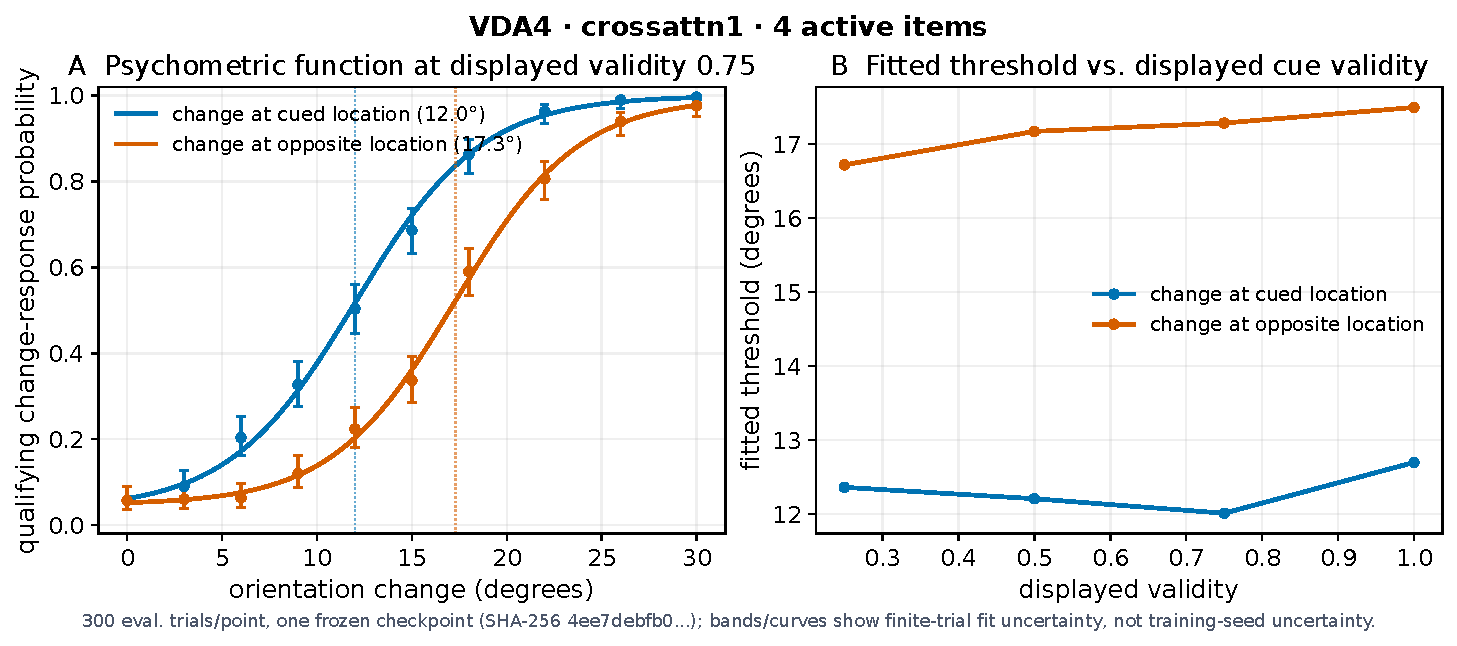
\includegraphics[width=0.485\textwidth]{psychometric_fit_vda4_crossattn1.pdf}\hfill
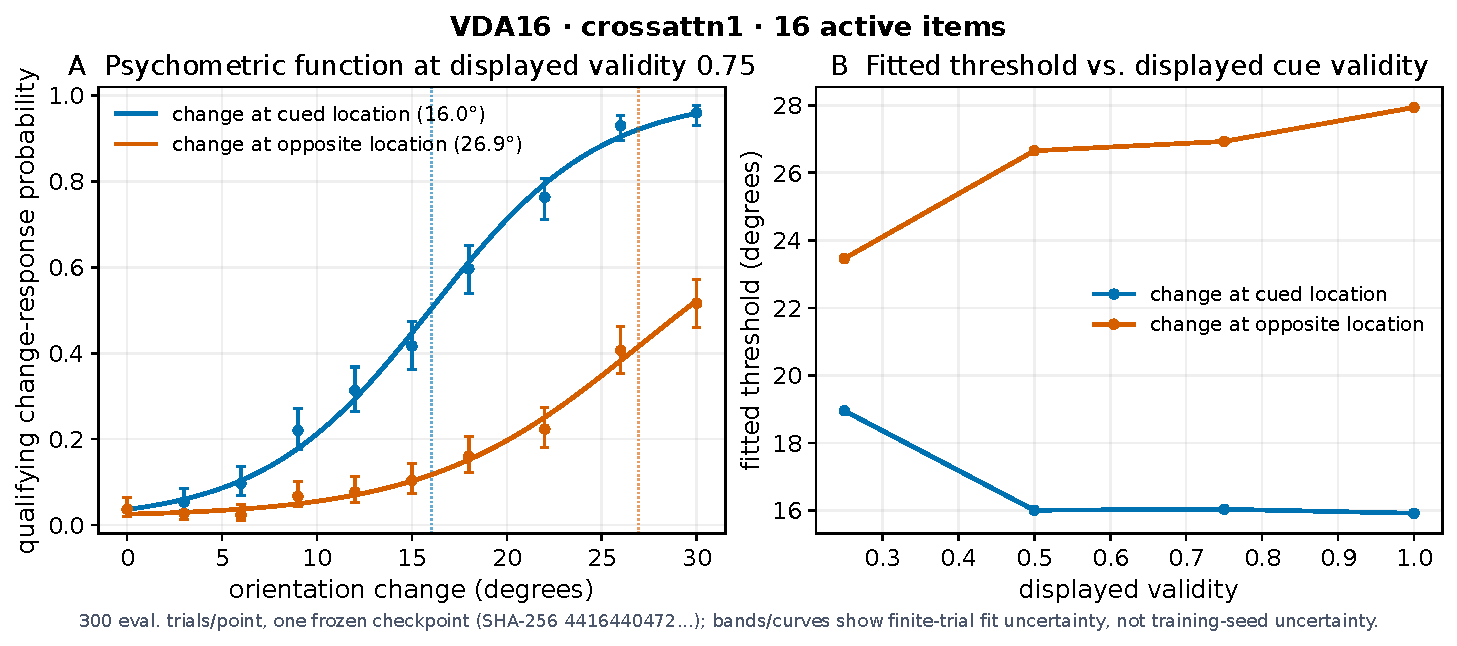
\includegraphics[width=0.485\textwidth]{psychometric_fit_vda16_crossattn1.pdf}\\[3pt]
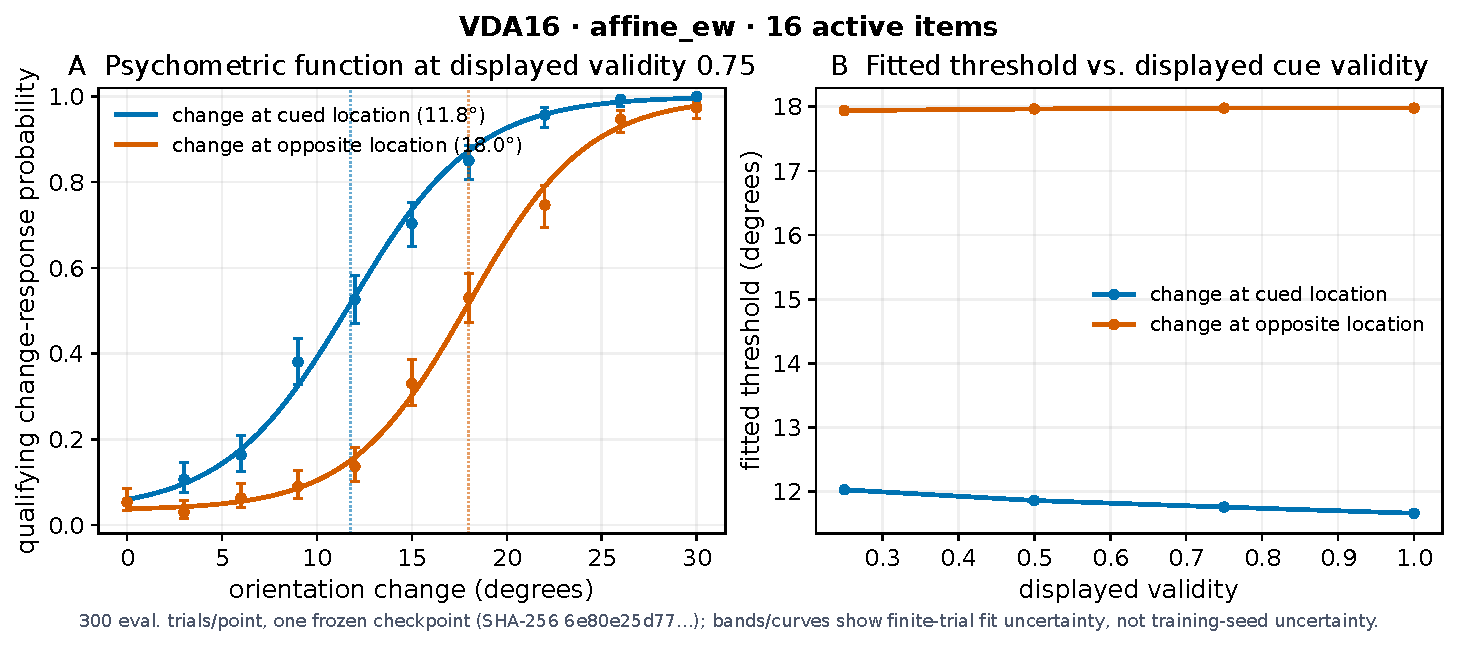
\includegraphics[width=0.485\textwidth]{psychometric_fit_vda16_affine_ew.pdf}
\caption{\textbf{Fitted psychometric functions and thresholds.} Top-left: VDA4 cross-attention (set size 4 baseline). Top-right: VDA16 cross-attention -- threshold separation roughly doubles relative to set size 4. Bottom: VDA16 affine -- separation is comparable to affine's own set-size-9 value, not double its set-size-4 value. Panel A: fitted function at displayed validity 0.75. Panel B: fitted threshold vs.\ displayed validity.}\label{fig:psych-fit}
\end{figure*}

\begin{figure}[t]
\centering
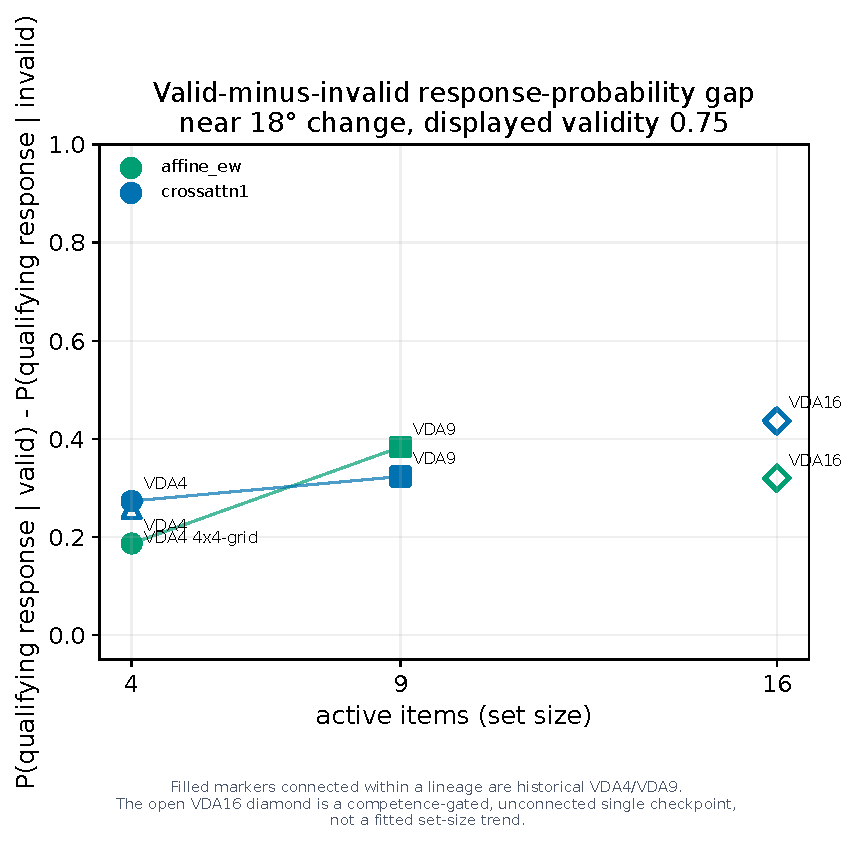
\includegraphics[width=\linewidth]{psychometric_fit_setsize_summary.pdf}
\caption{\textbf{Cueing-effect magnitude vs.\ set size, by routing family.} Valid-minus-invalid response-probability gap near $18^\circ$, displayed validity 0.75. Filled markers connected within the historical VDA4/VDA9 lineage; open VDA16 diamonds are competence-gated, differently lineaged single checkpoints plotted unconnected.}\label{fig:psych-fit-summary}
\end{figure}

\begin{figure*}[t]
\centering

\includegraphics[width=0.85\textwidth]{vda_method_comparison_with_vda16.pdf}
\caption{\textbf{Behavioral and representational context across the full set-size series.} (A) Valid-minus-invalid response rate. (B--C) Final-timestep decoders. (D) No-change false-alarm rate, which stays low and does not rise with set size -- evidence against the simplest criterion-only account of the widening gap in (A). Open VDA16 markers are competence-gated, unconnected points, not a fitted trend.}\label{fig:vda16-context}
\end{figure*}

\subsection{Is the base cueing effect sensitivity, criterion, or both?}\label{sec:baseline-sdt}
Figure~\ref{fig:vda16-context}D already shows the false-alarm rate stays low and flat across set size -- evidence against a criterion-only account of the widening response-rate gap, but not a full decomposition. Luo and Maunsell's warning applies directly here: a response-probability gap alone cannot distinguish a model that discriminates the change better when cued from one that simply becomes more willing to declare ``change'' \cite{luo2018}. Every clamp analysis in this paper already reports $d'$ and criterion because computing either requires a false-alarm rate, which those analyses compute as a byproduct of their no-change condition; the plain psychometric curves in Section~\ref{sec:behavior} never added that arm. We close that gap here for both VDA16 checkpoints -- the only checkpoints in this paper with a real, hash-verified local file available to run one -- by adding 300 fresh no-change trials per displayed validity (no clamp, same trial structure otherwise) and combining the resulting false-alarm count with the already-cached, already-verified hit counts behind Figure~\ref{fig:vda16-context}A, via the identical $d'=\Phi^{-1}(H)-\Phi^{-1}(F)$, $c=-\tfrac12[\Phi^{-1}(H)+\Phi^{-1}(F)]$ used throughout Section~\ref{sec:intervention}.

At displayed validity 0.75 and $18^\circ$ -- the same focal point already quoted in Section~\ref{sec:vda16-behavior} -- \textbf{the base cueing effect is substantially a sensitivity effect for both routing families, not just a criterion shift, though the two families differ in how much.} Cross-attention's $d'$ rises from $0.56$ (invalid) to $1.80$ (valid), a $3.2\times$ ratio; its criterion falls from $1.27$ to $0.66$, roughly halving. Affine's $d'$ rises from $2.01$ to $2.97$, only a $1.5\times$ ratio, while its criterion falls from $0.93$ to $0.45$ -- almost exactly the same halving cross-attention shows (Figure~\ref{fig:baseline-sdt}). Criterion moves by a similar proportion in both routing families; sensitivity does not -- cross-attention's cueing benefit leans harder on a genuine discriminability gain, consistent with it being the routing family whose cueing benefit also grows with set size (Section~\ref{sec:psychometric-fits}). \note{This decomposition currently covers only the two VDA16 checkpoints, because they are the only checkpoints in this paper with a locally available \texttt{.pt} file to add a no-change arm to; the first-wave VDA4/VDA9 and width-comparison psychometrics in Section~\ref{sec:behavior} report response probability only, for the same missing-checkpoint reason recorded throughout this paper. Extending this decomposition to those points, or to the two VDA4 checkpoints trained for this paper's later sections, is future work.}

\begin{figure*}[t]
\centering
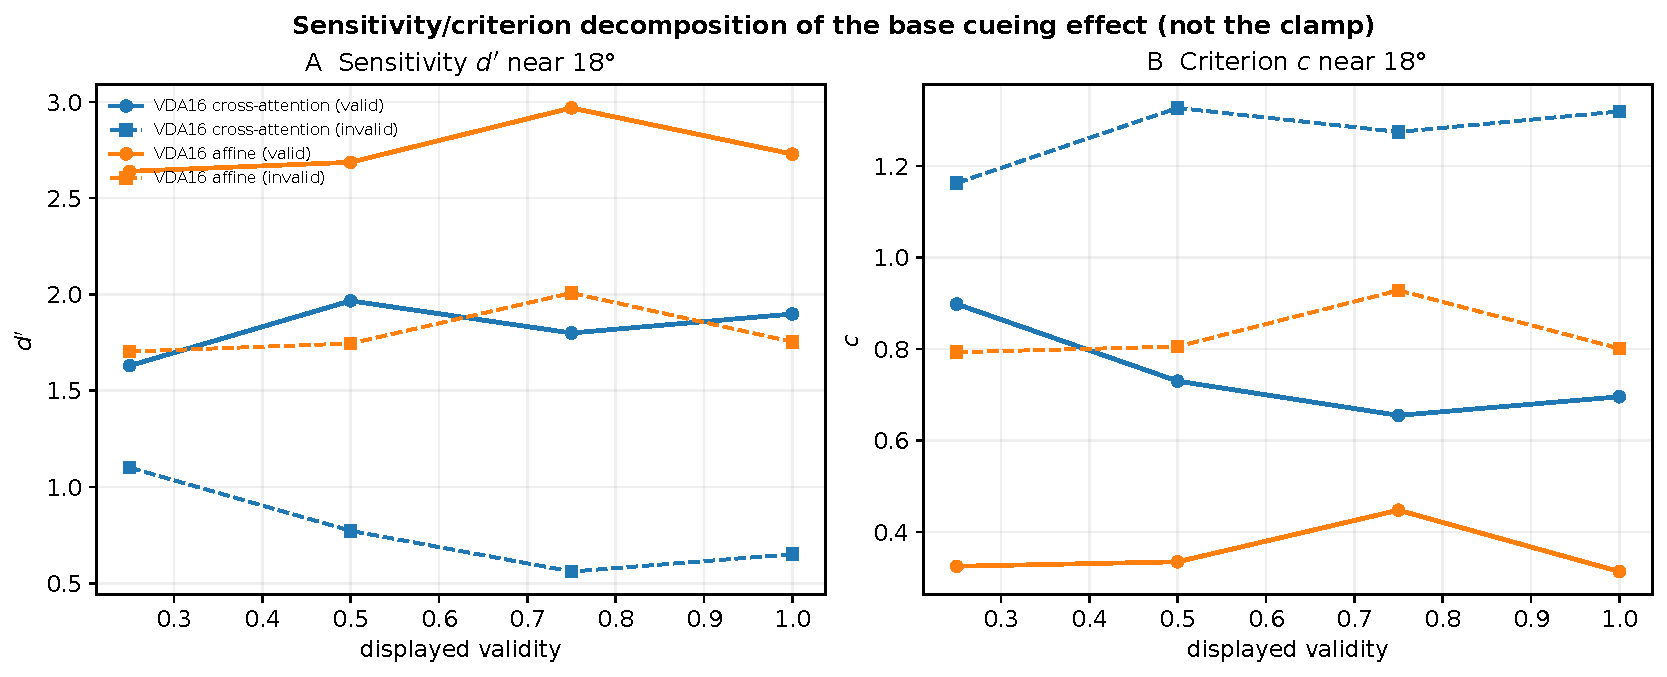
\includegraphics[width=0.85\textwidth]{baseline_sdt_decomposition.pdf}
\caption{\textbf{Sensitivity and criterion behind the base cueing effect, not the clamp.} Same $d'$/$c$ decomposition used for every intervention result in this paper (Section~\ref{sec:intervention}), applied for the first time to the unmanipulated psychometric curves themselves. Solid: valid trials. Dashed: forced-invalid trials. Both routing families show a real sensitivity gap between valid and invalid trials, not only a criterion shift, but cross-attention's is proportionally larger.}\label{fig:baseline-sdt}
\end{figure*}

\FloatBarrier
\section{Attention Dynamics Over Time}\label{sec:attention-dynamics}
A cueing benefit could in principle arise without the model's internal routing ever tracking the cue. This section asks where routing weight actually goes across the trial timeline -- blank, cue, delay, array, change, response -- and what a held-out linear probe can decode from the recurrent state at each point, following the same event-alignment discipline Herman and Krauzlis used to relate superior-colliculus activity to detection \cite{herman2017,carrasco2011}. Throughout, ``attention map'' names the model's own routing weights over locations, not a claim about a literal neural attention map.

\subsection{Event-aligned attention maps at set sizes 4 and 9}\label{sec:first-wave-attention}
Each map evaluates four displayed cue proportions on 96 matched no-change trials each: the cue is fixed, nothing ever changes, and t5 is retained only as the nominal change opportunity. Affine exposes one spatial-key array; cross-attention exposes separate image-key and recurrent-memory-key arrays (Figure~\ref{fig:first-wave-attn}).

\begin{figure*}[t]
\centering
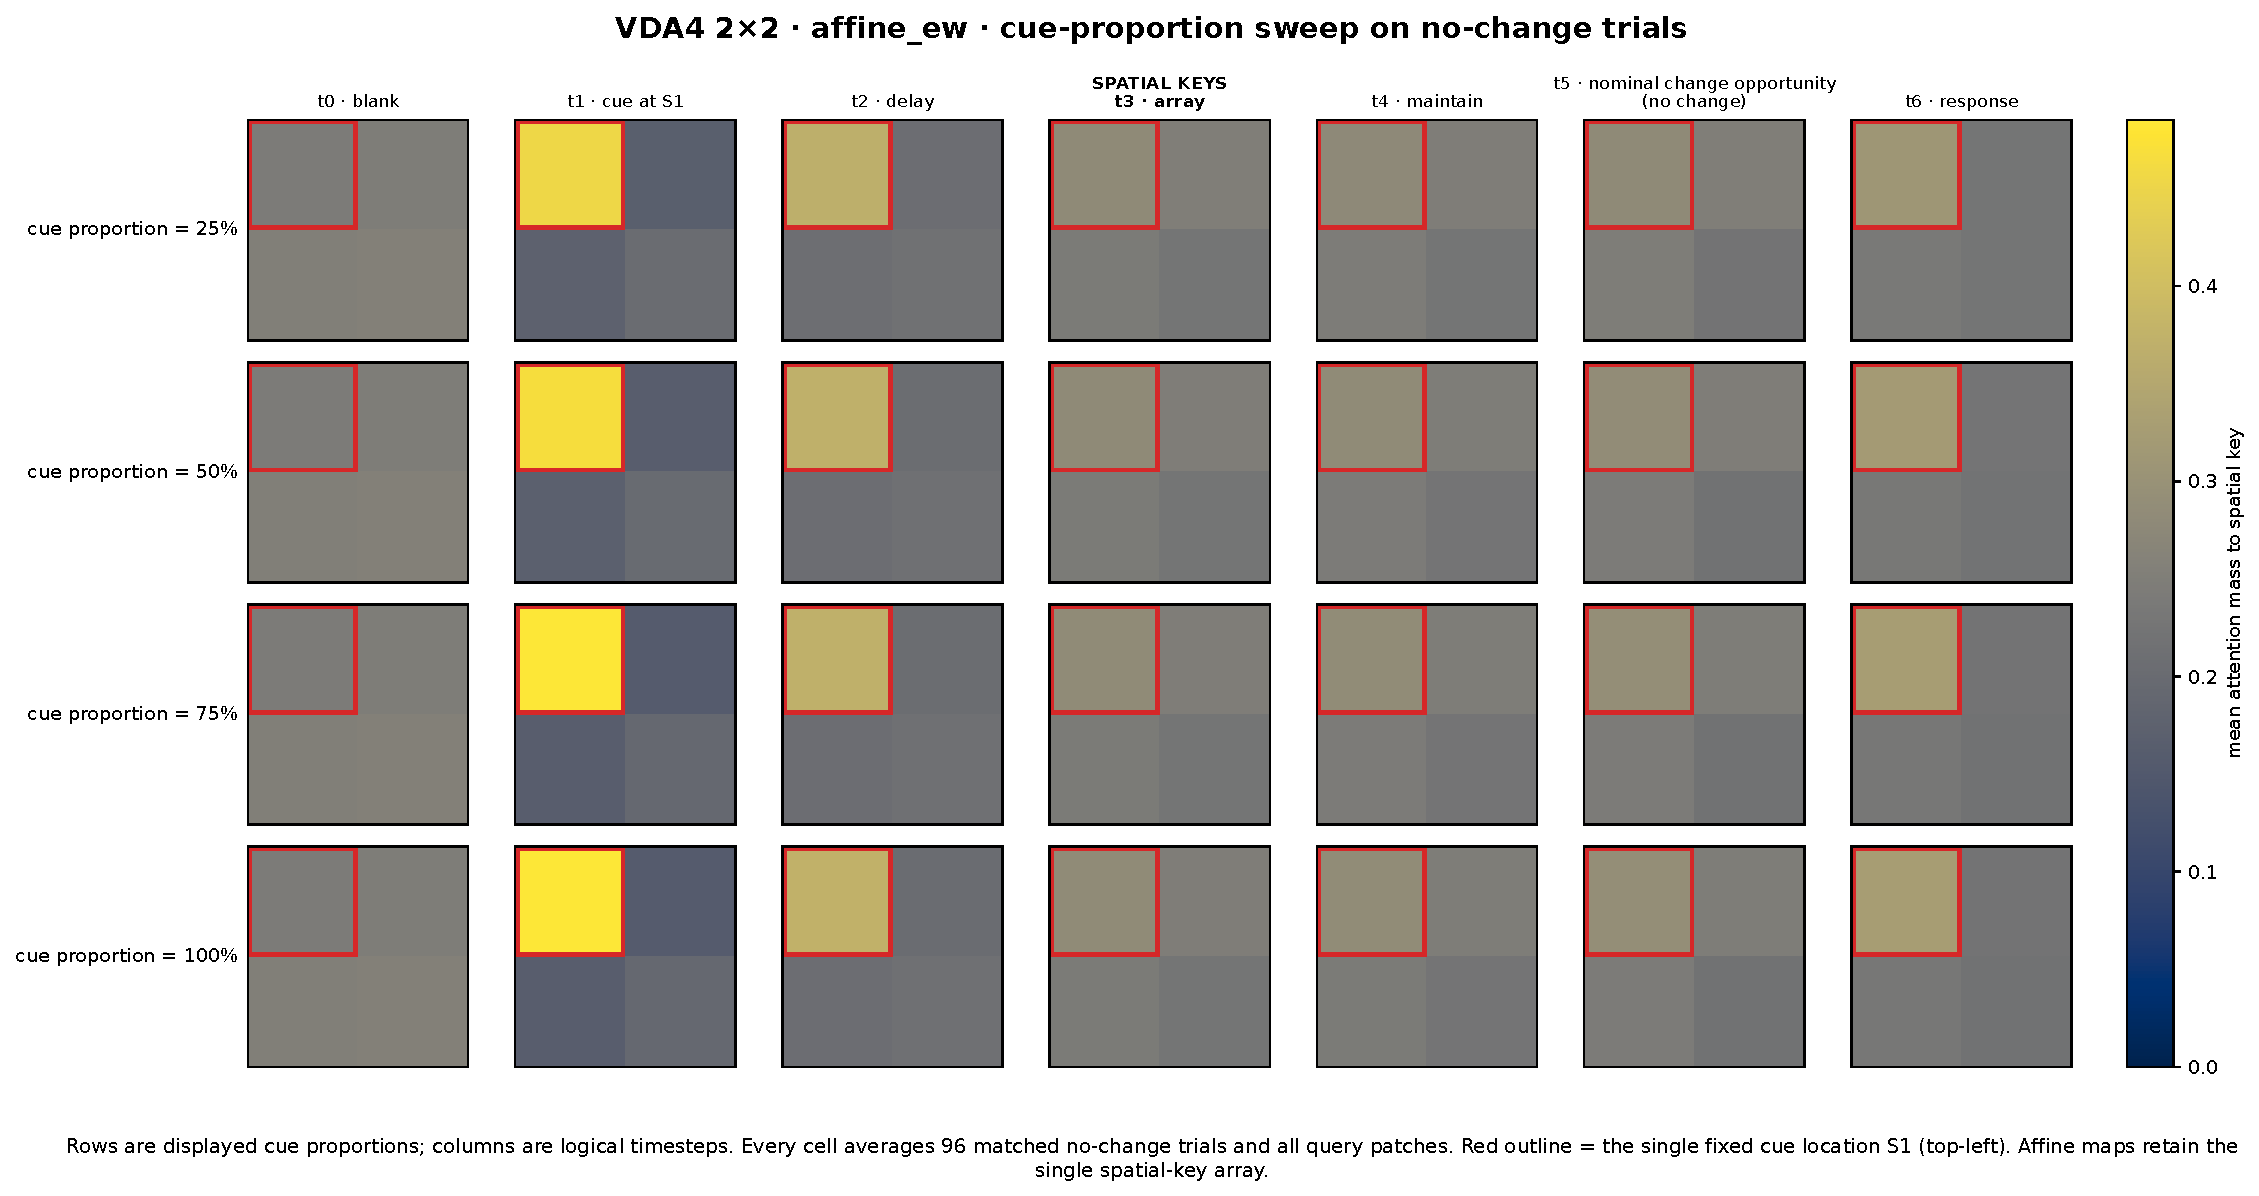
\includegraphics[width=0.32\textwidth]{first_wave_attention_vda4_affine_ew.pdf}\hfill
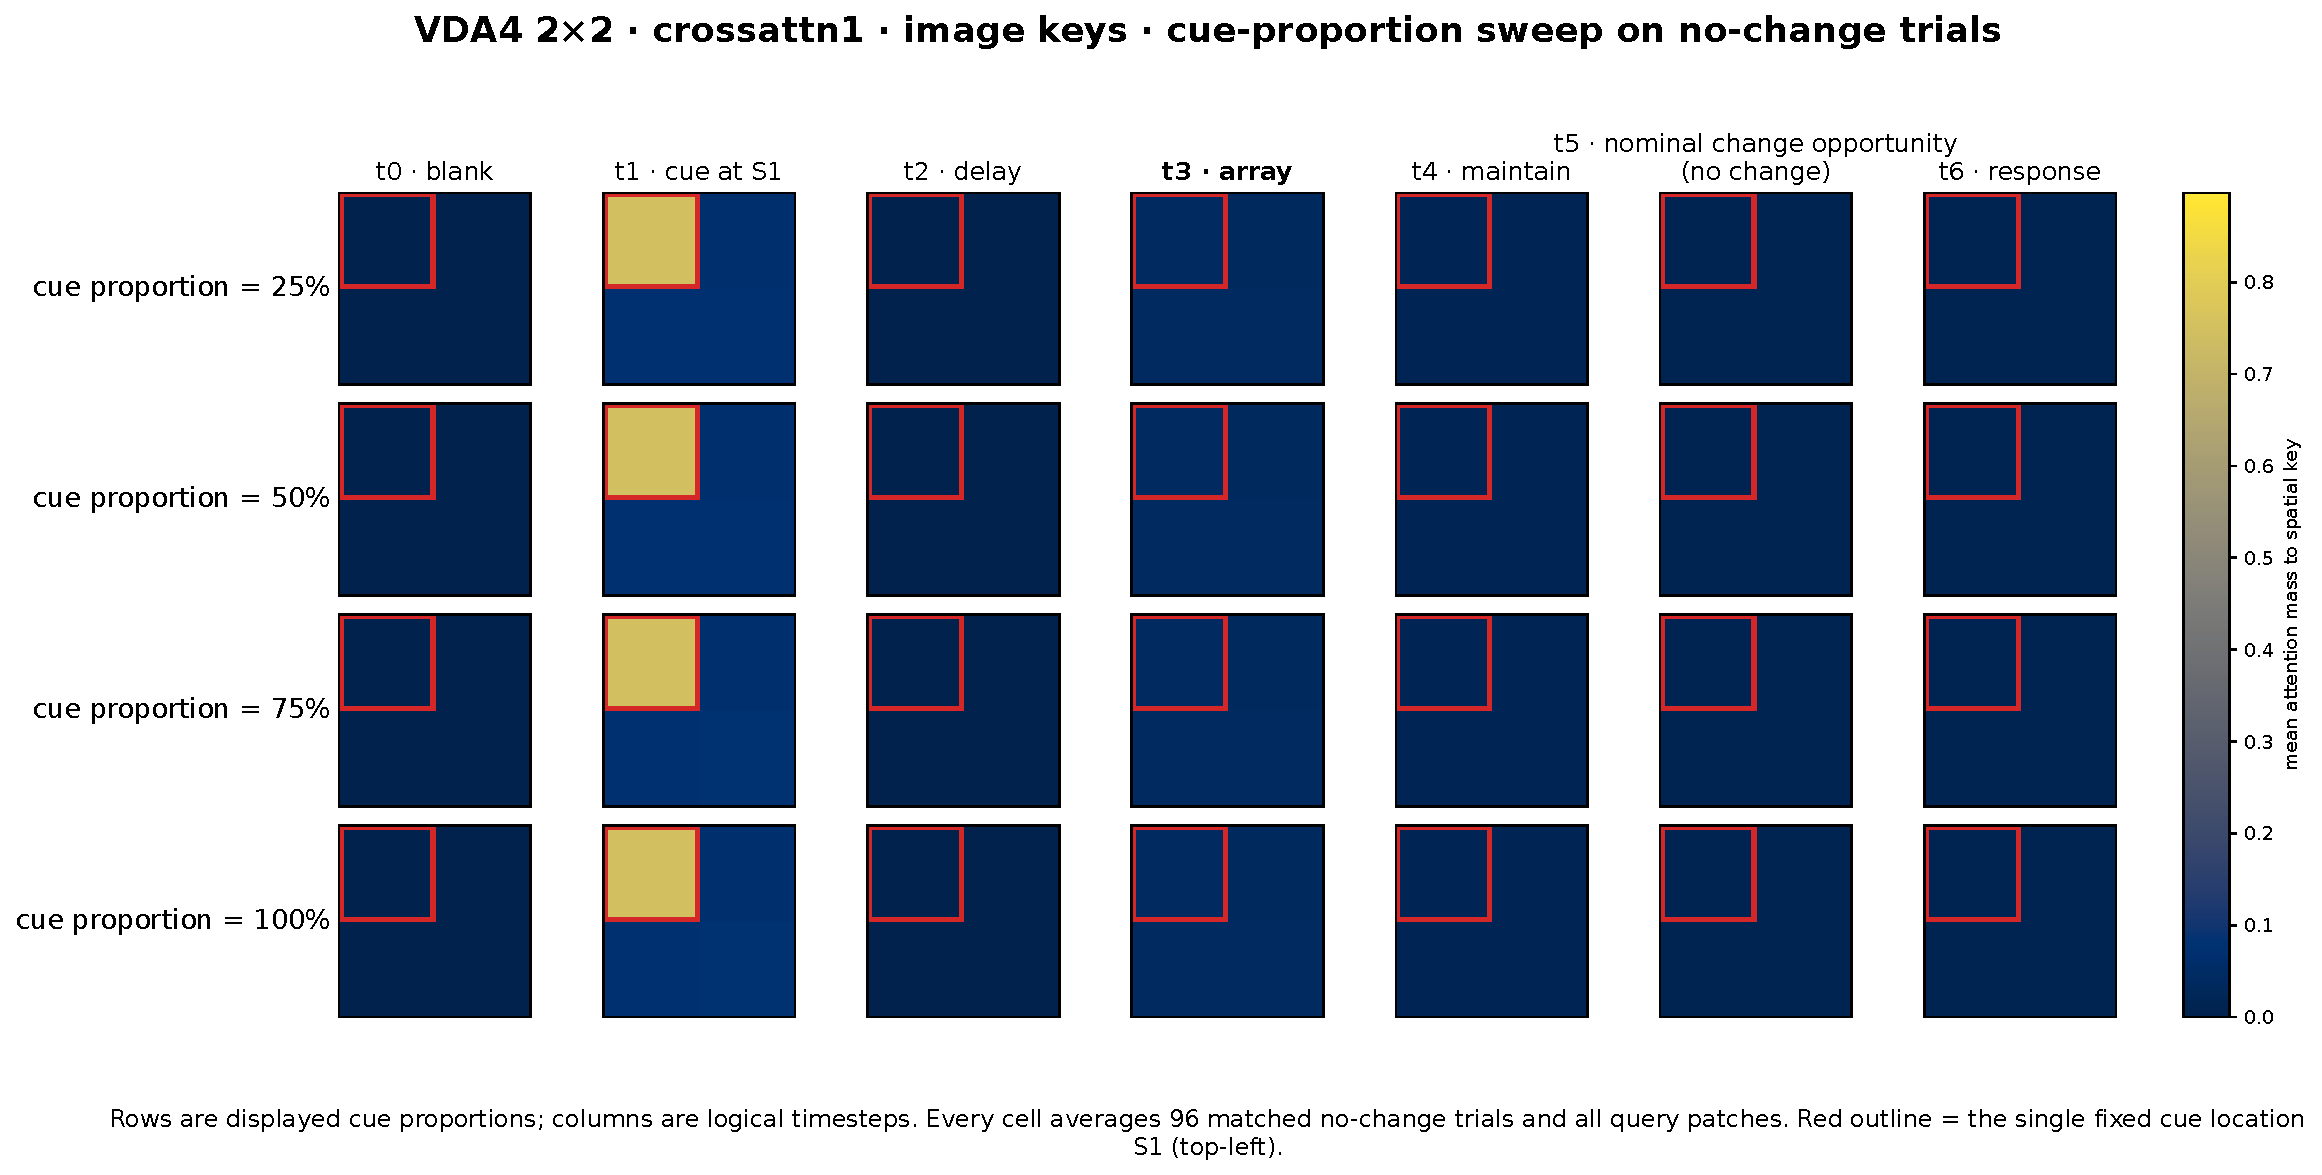
\includegraphics[width=0.32\textwidth]{first_wave_attention_vda4_crossattn1_image_keys.pdf}\hfill
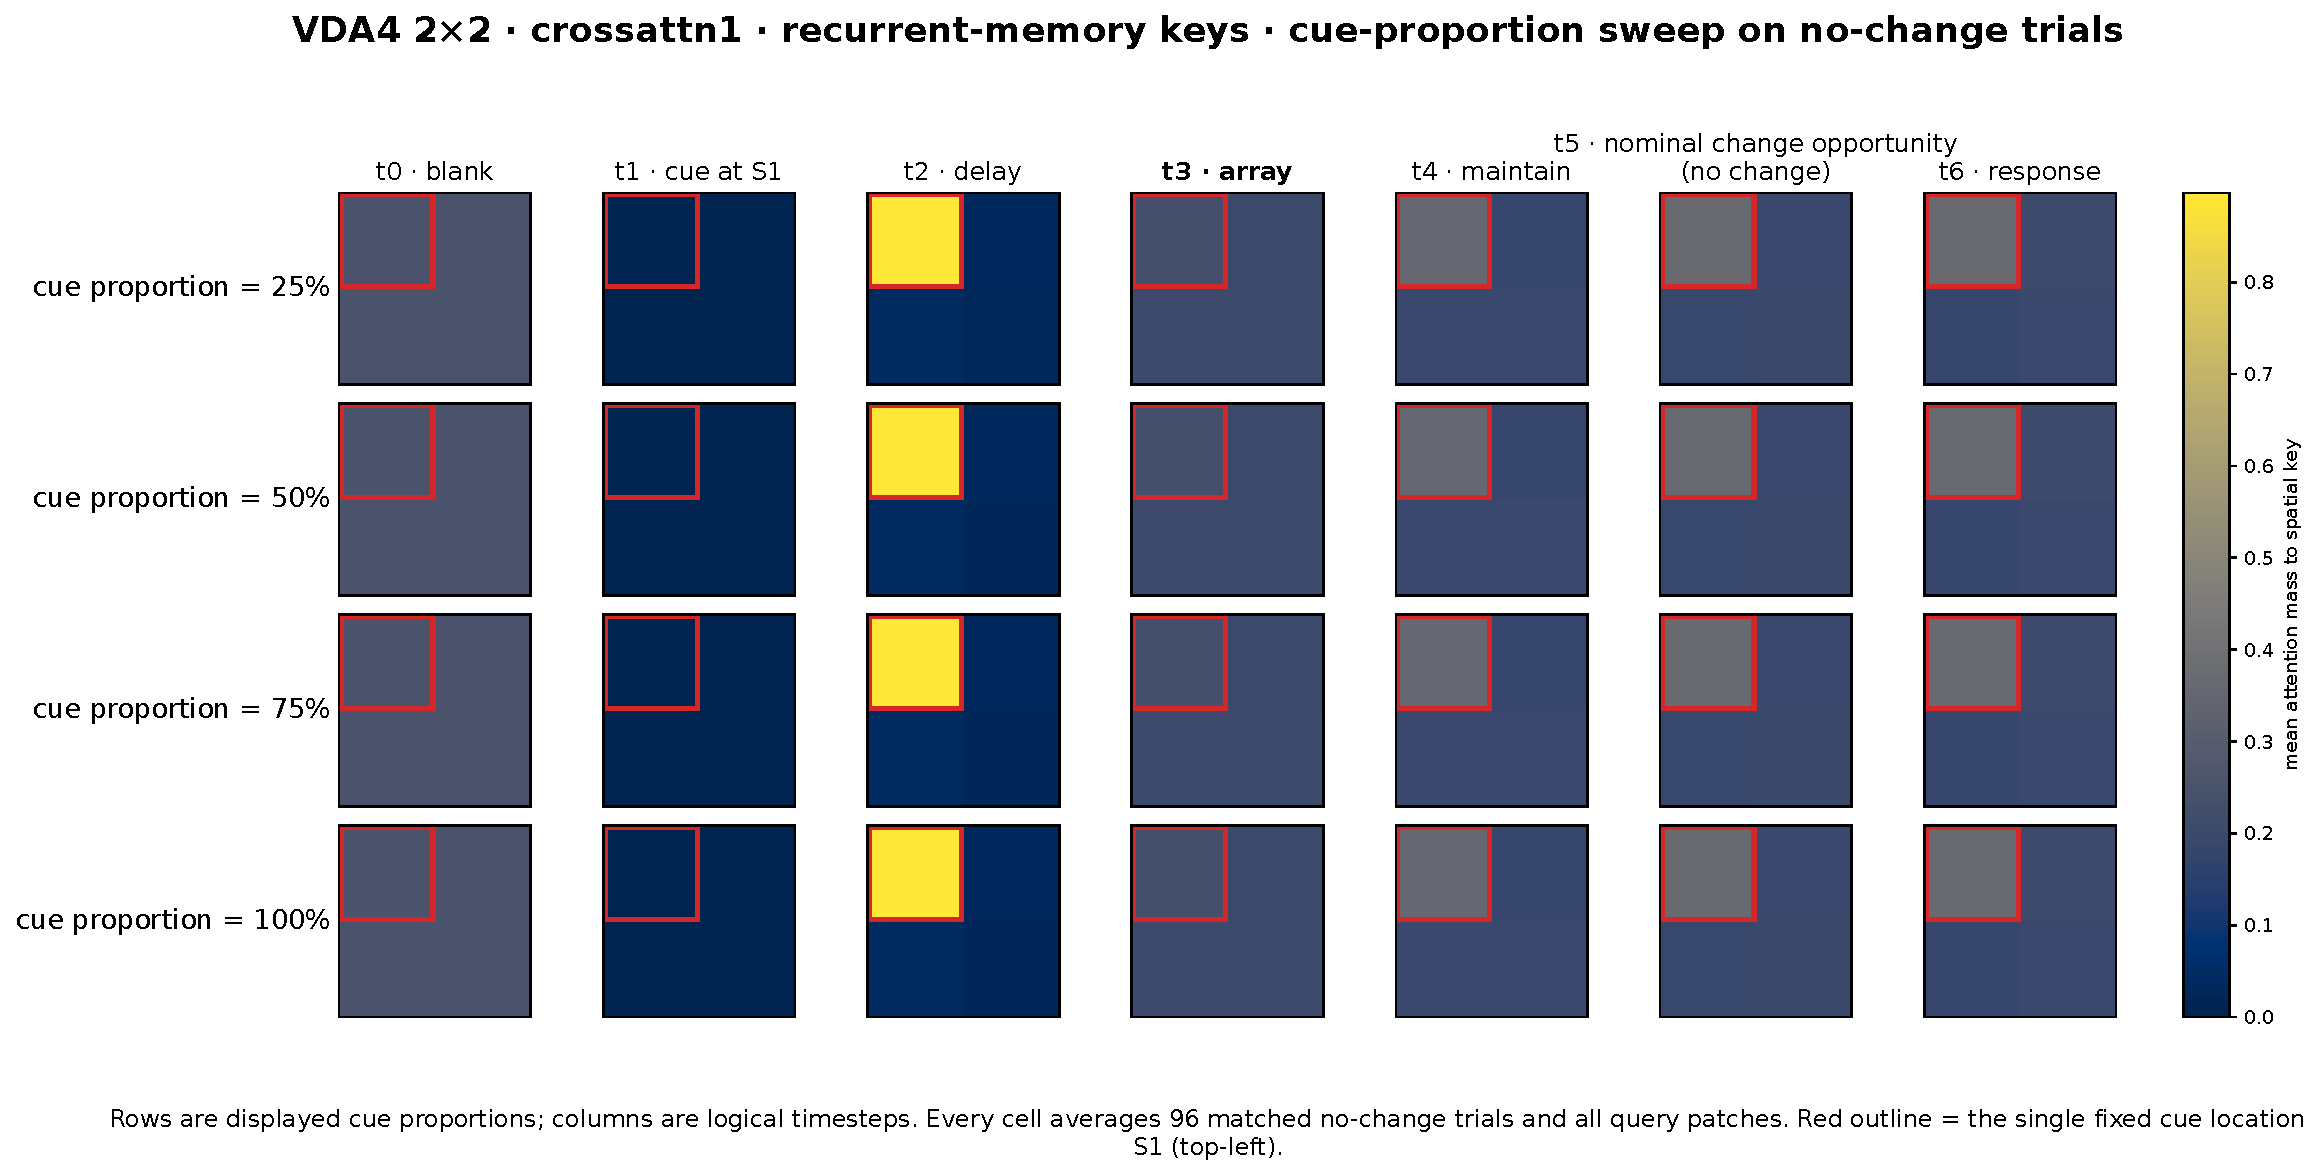
\includegraphics[width=0.32\textwidth]{first_wave_attention_vda4_crossattn1_recurrent_memory_keys.pdf}\\[4pt]
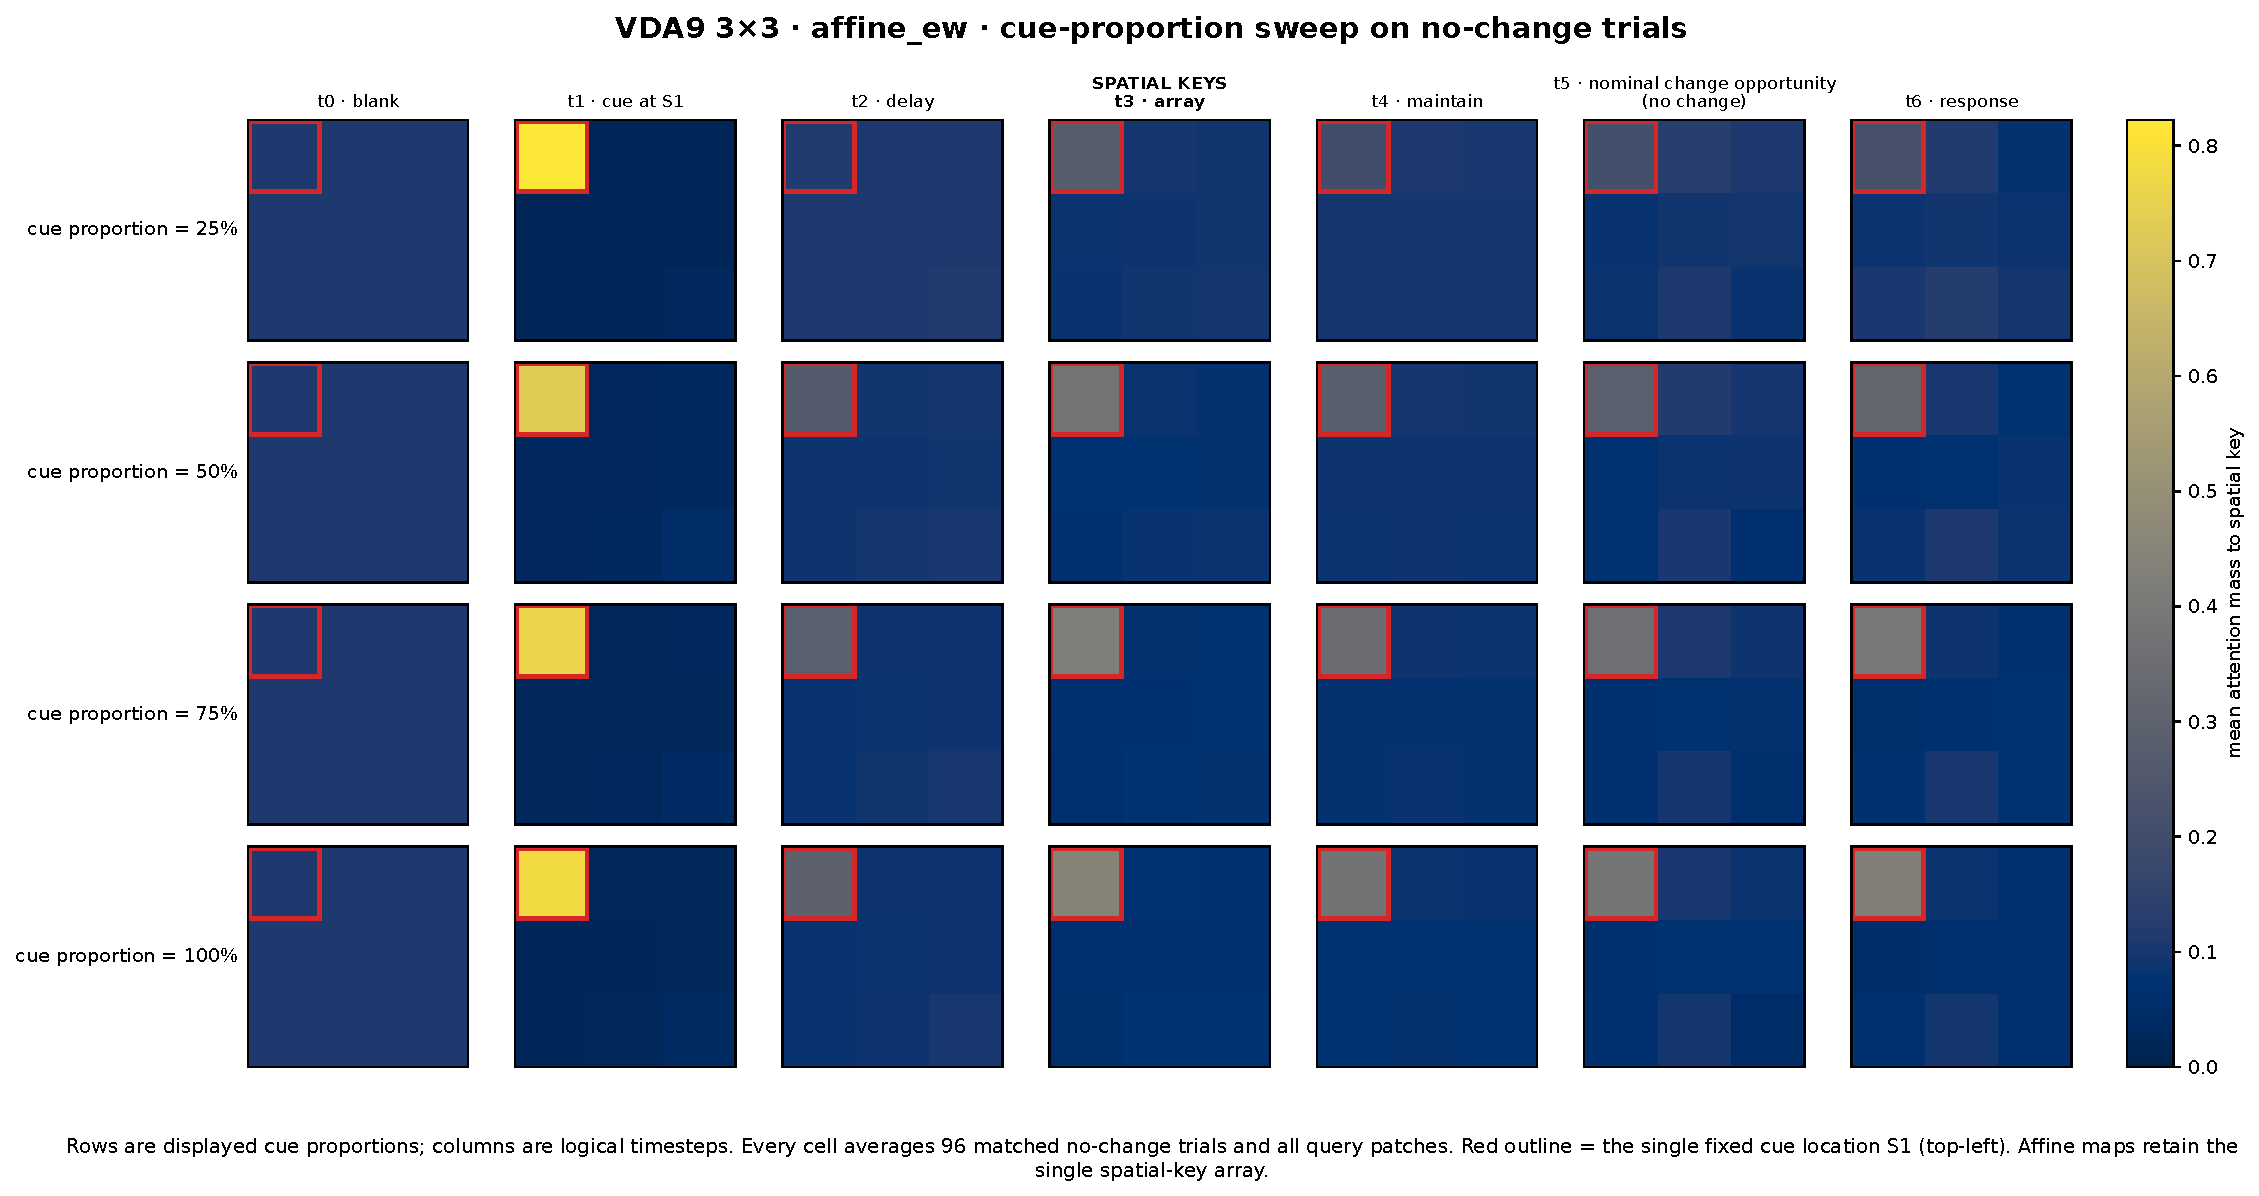
\includegraphics[width=0.32\textwidth]{first_wave_attention_vda9_affine_ew.pdf}\hfill
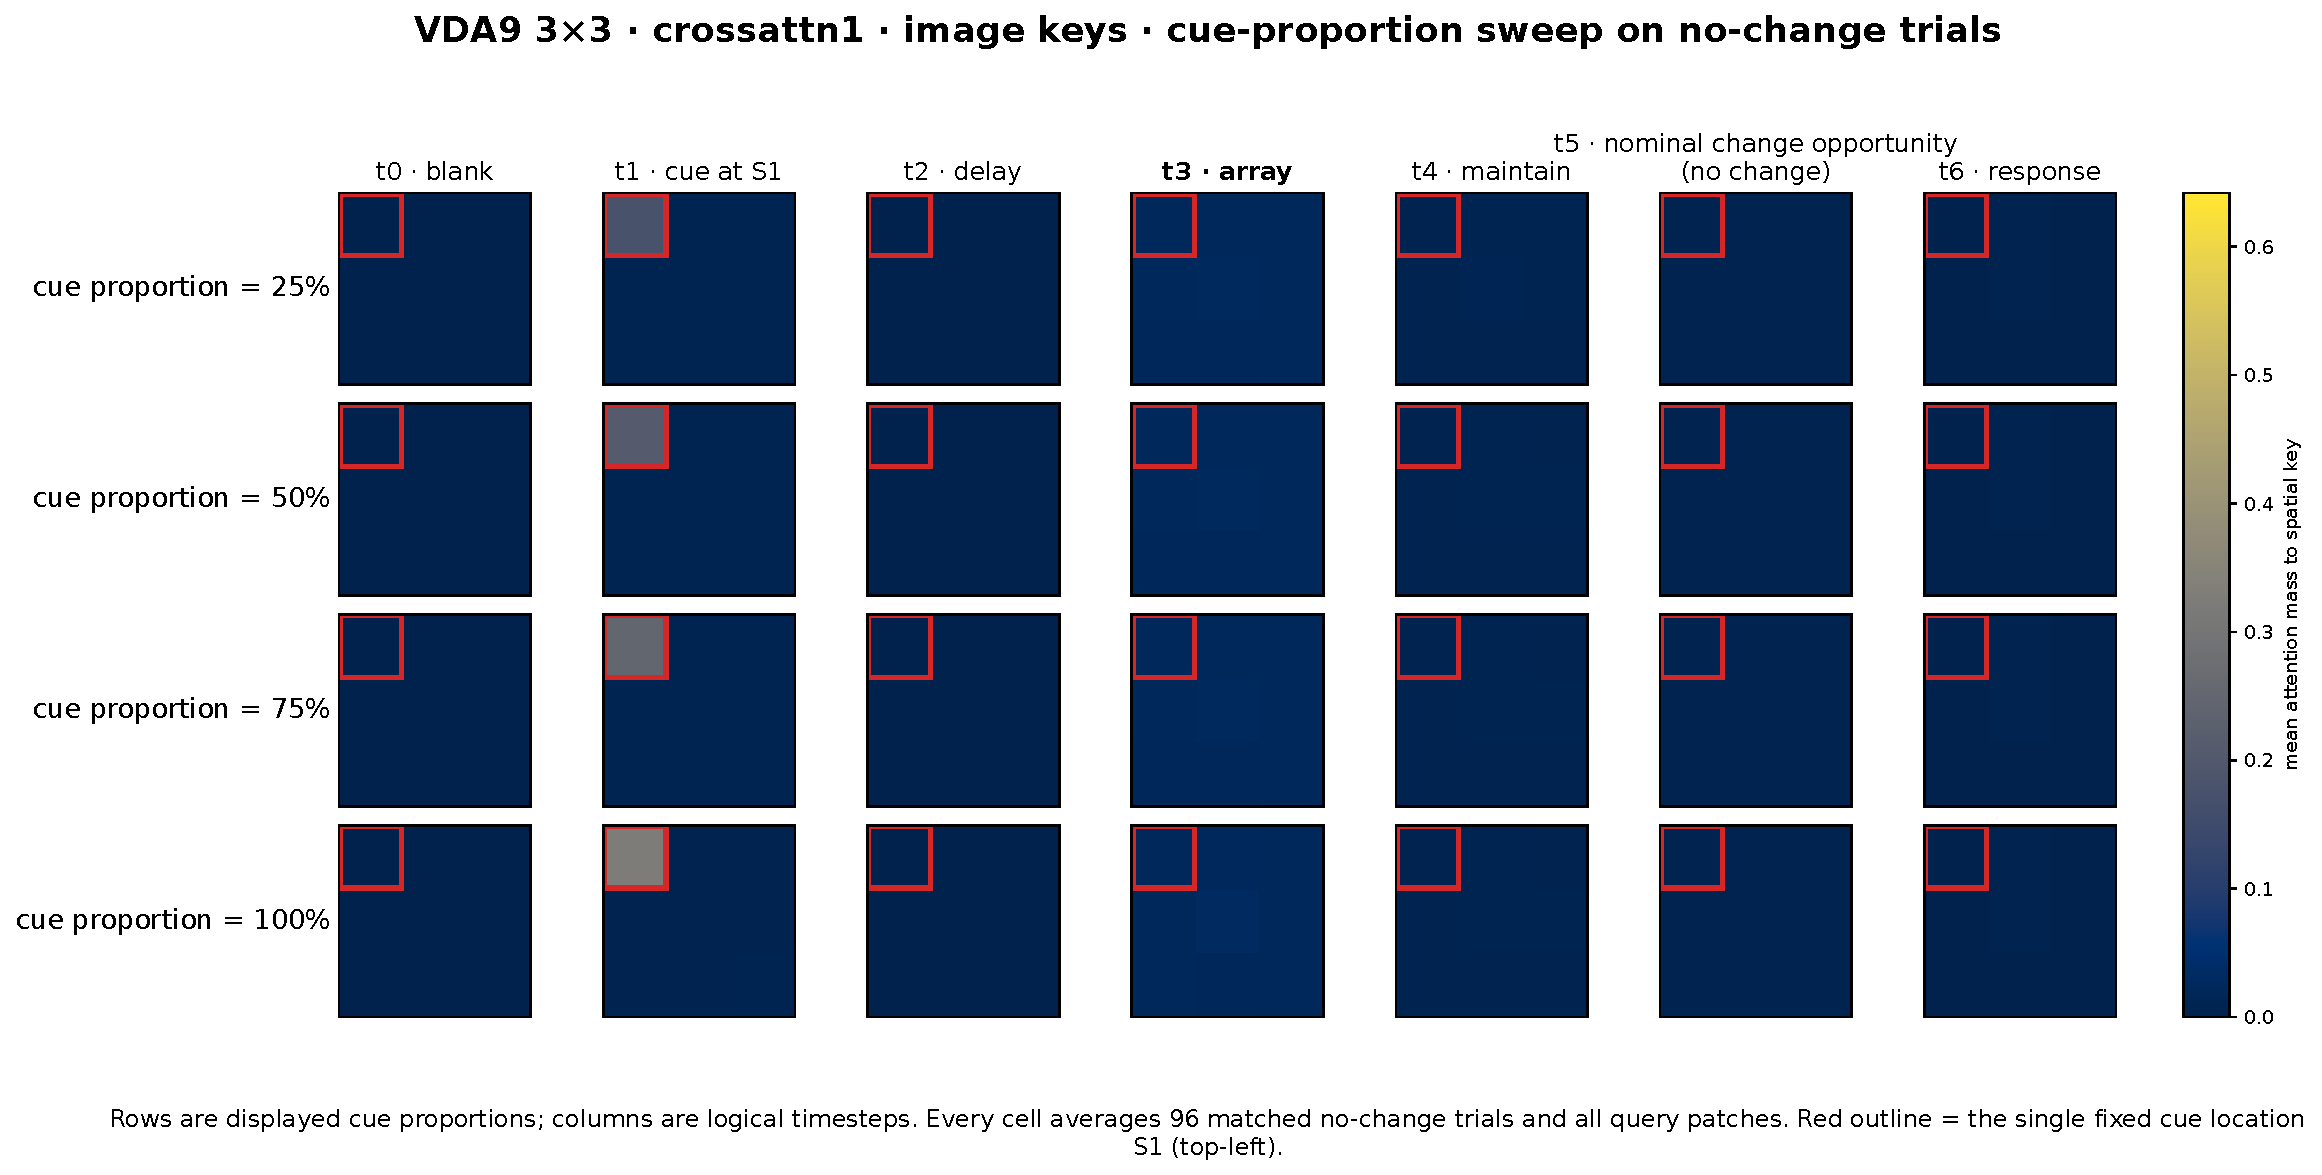
\includegraphics[width=0.32\textwidth]{first_wave_attention_vda9_crossattn1_image_keys.pdf}\hfill
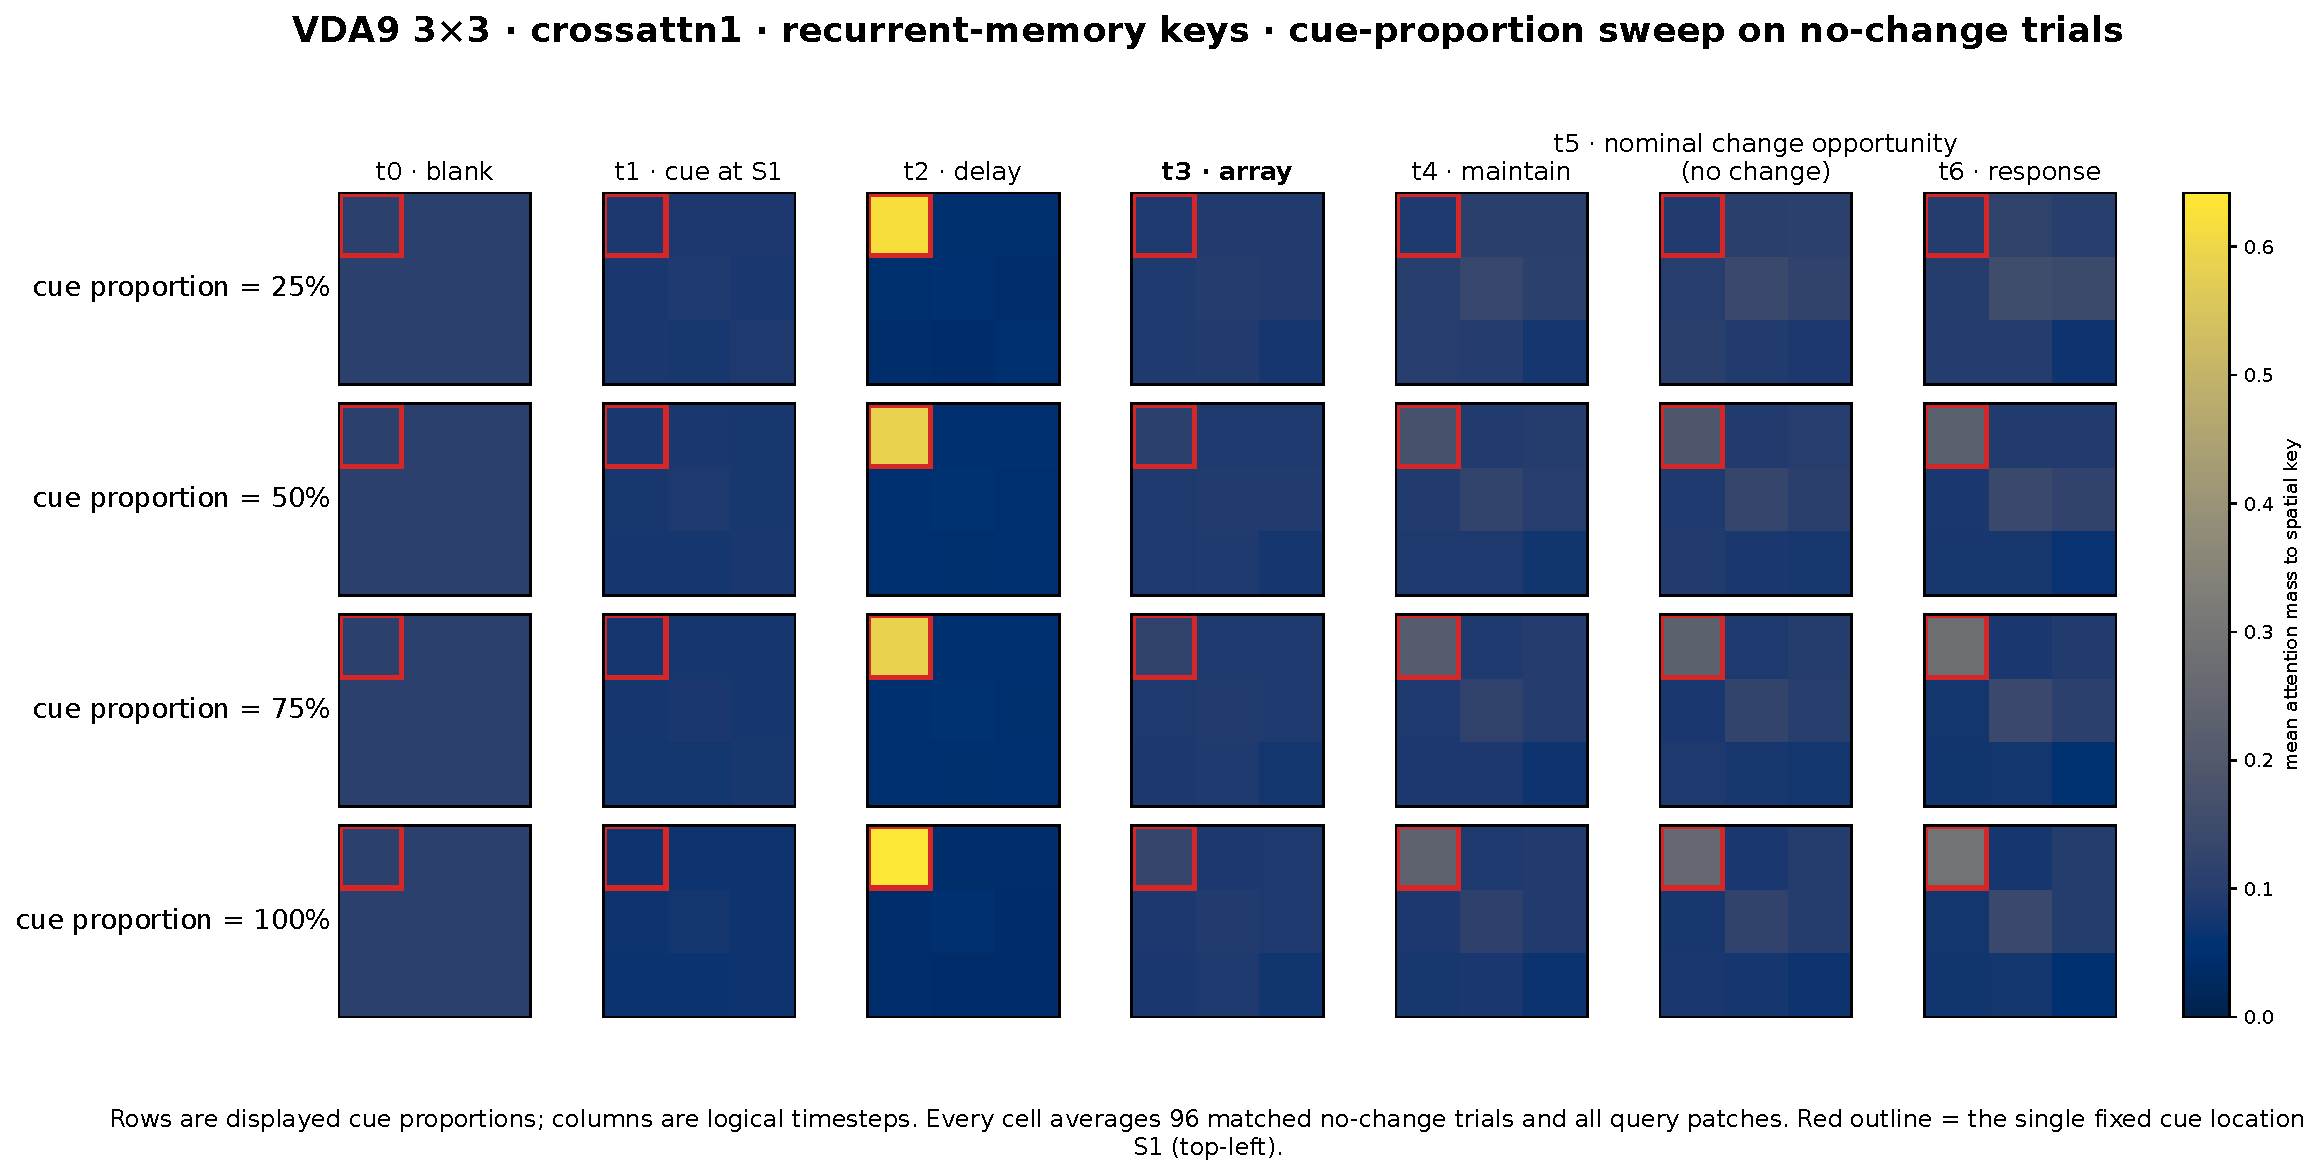
\includegraphics[width=0.32\textwidth]{first_wave_attention_vda9_crossattn1_recurrent_memory_keys.pdf}
\caption{\textbf{No-change-trial attention maps, VDA4 (top) and VDA9 (bottom).} Left to right: affine self-attention, cross-attention image keys, cross-attention memory keys. Rows are displayed cue proportion, columns are logical timesteps t0--t6; a red outline marks the fixed cue location. Because no physical change ever occurs, this evidence is completed by the paired VDA16 change-trial experiment in Section~\ref{sec:vda16-paired-attention}.}\label{fig:first-wave-attn}
\end{figure*}

\subsection{What a held-out probe reads from the recurrent state}\label{sec:width-decoding}
A regularized logistic probe, fit within each fold on train-only PCA-reduced state, reads change occurrence robustly everywhere (t6 balanced accuracy 0.76--0.90; Table~\ref{tab:decoder-scores}) and change location more variably (0.50--0.96, well above the relevant chance level). d256-minus-d128 differences vary in sign across pairs -- VDA4 affine gains 0.285 for change-location decoding, VDA4 cross-attention \emph{loses} 0.050 -- so \textbf{a wider checkpoint does not expose uniformly more decodable information} either, the representational counterpart to Section~\ref{sec:width-behavior}. \note{These scores establish information available to a linear readout at t6; they establish neither policy use nor persistent maintenance, and per Panichello and Buschman we do not claim a domain-general controller from a single task's decoder \cite{panichello2021}.}

\begin{table}[t]
\centering\small
\begin{tabularx}{\linewidth}{@{}l l Y Y@{}}
\toprule
Task & Routing & Change occ.\ (d128/d256) & Change loc.\ (d128/d256)\\
\midrule
VDA1 & affine & .893/.902 & undefined\\
VDA1 & cross-attn & .897/.888 & undefined\\
VDA4 & affine & .830/.879 & .616/.900\\
VDA4 & cross-attn & .818/.833 & .842/.792\\
VDA9 & affine & .761/.792 & .654/.499\\
\bottomrule
\end{tabularx}
\caption{Final-timestep (t6) held-out decoder balanced accuracy. Location targets undefined for singleton VDA1.}\label{tab:decoder-scores}
\end{table}

\subsection{VDA16 attention maps and readout}\label{sec:vda16-attention-dynamics}
The same no-change protocol at set size 16 shows the strongest cue-localized mass in cross-attention's recurrent-memory source at t2 -- after the cue, before the array -- while image-key cue mass at t1 grows with displayed cue proportion; affine's single self-attention array shows a strong S1 concentration at cue onset that persists, more weakly, through delay, array, and response (Figure~\ref{fig:vda16-attn}). A sustained cue-directed elevation during an empty delay is the pattern Awh and Jonides's overlapping-mechanisms account predicts if spatial attention supports rehearsal \cite{awh2001} -- \note{routing mass during delay is suggestive, not proof of rehearsal in the behavioral sense, which needs a delay-period disruption test we have not run.}

\begin{figure*}[t]
\centering

\includegraphics[width=0.32\textwidth]{first_wave_attention_vda16_crossattn1_image_keys.pdf}\hfill

\includegraphics[width=0.32\textwidth]{first_wave_attention_vda16_crossattn1_recurrent_memory_keys.pdf}\hfill
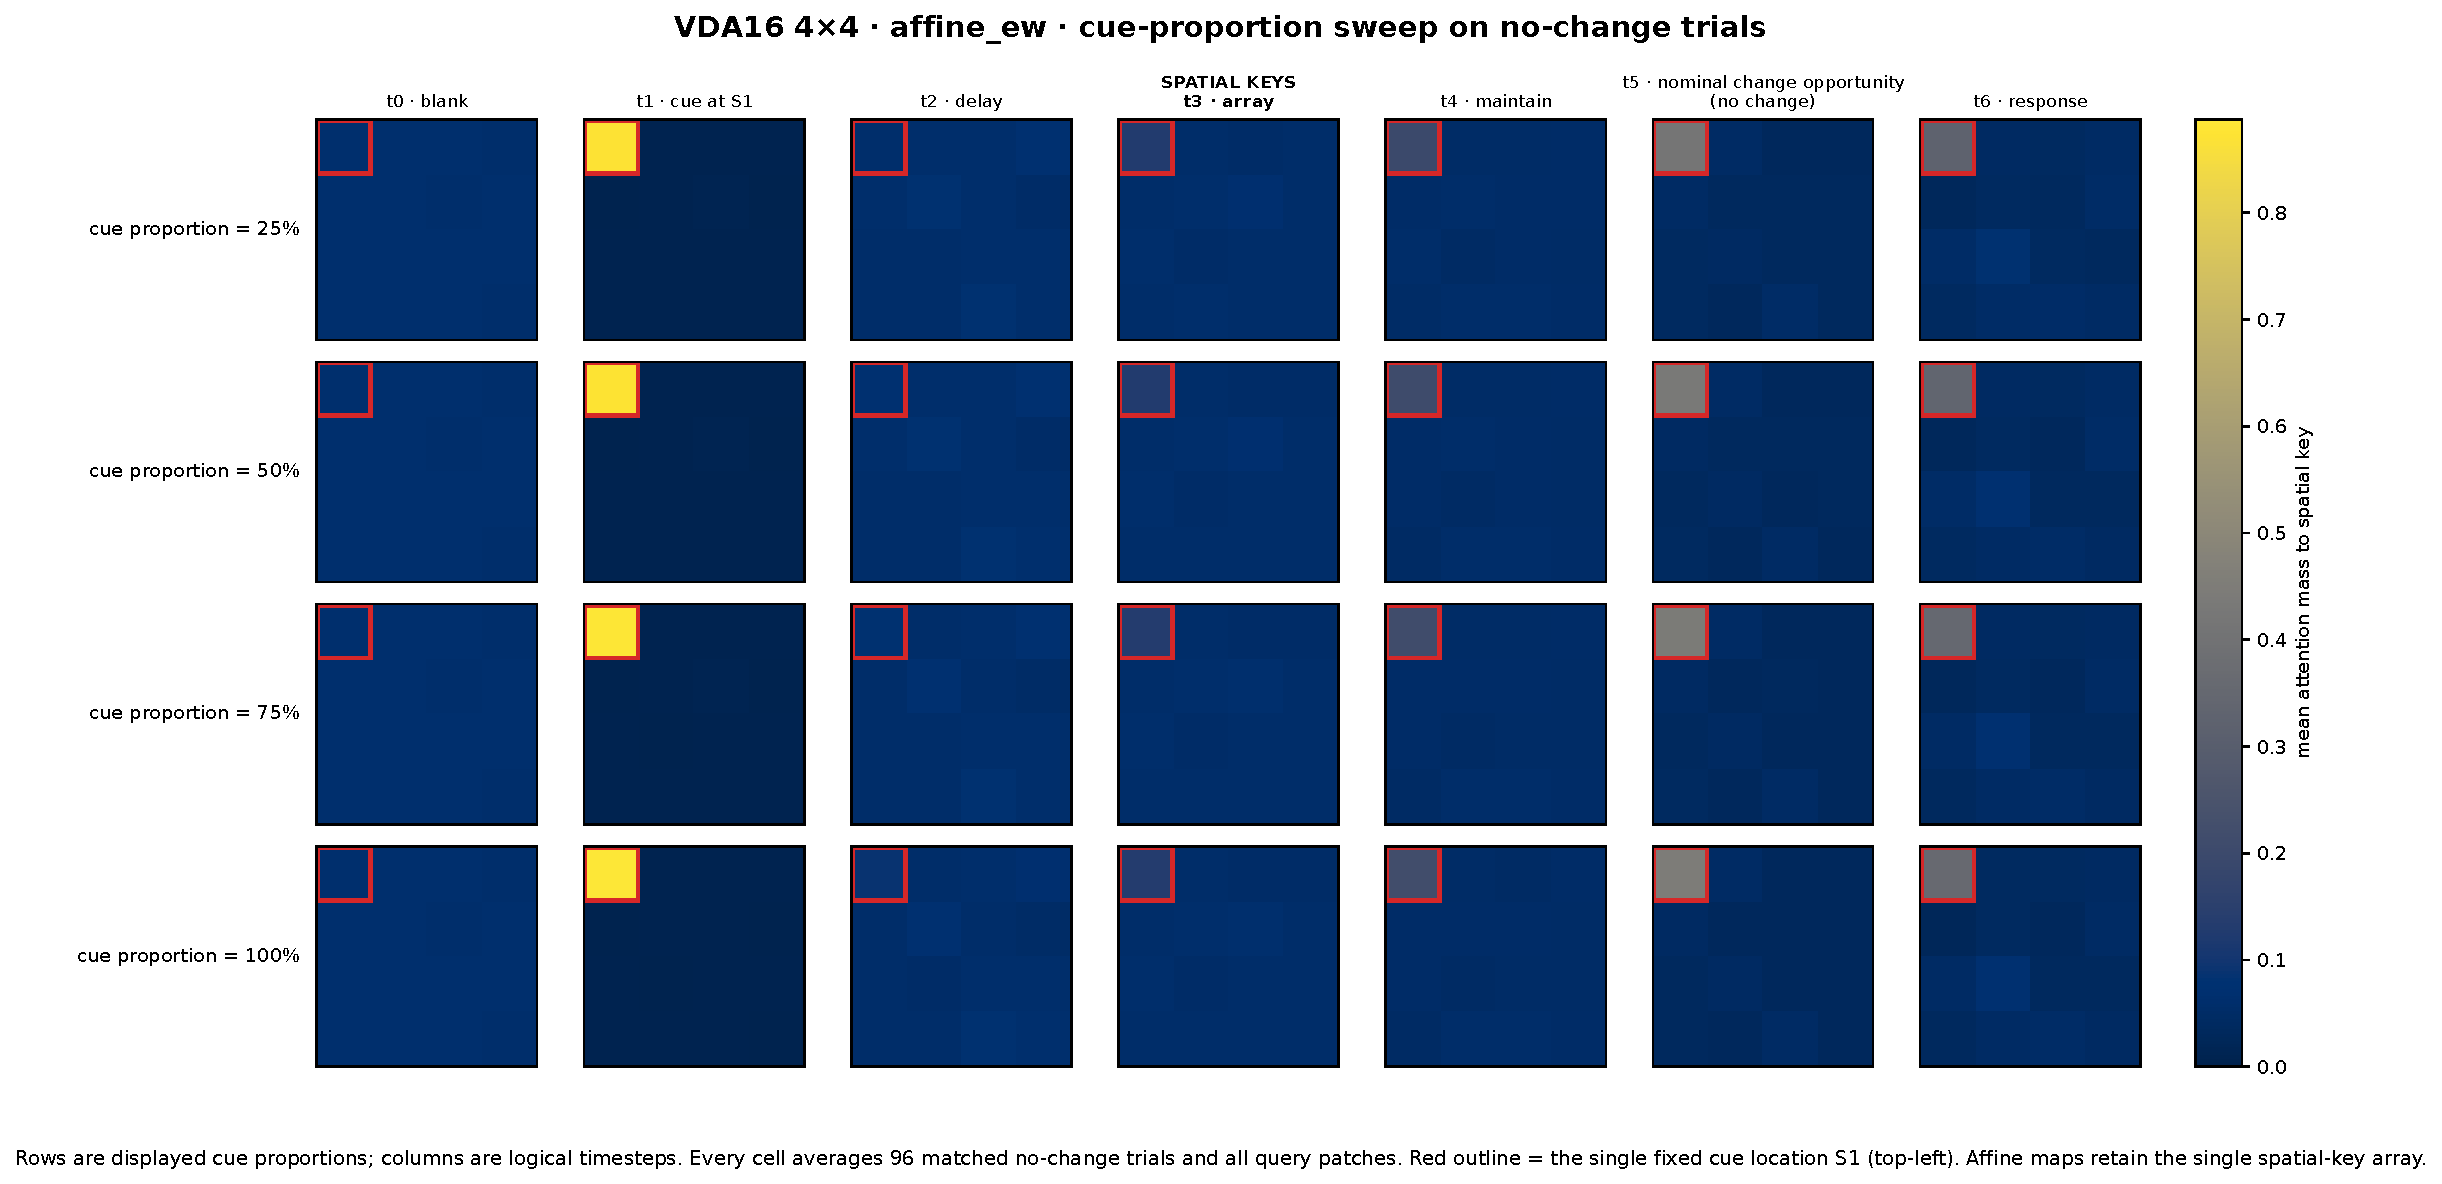
\includegraphics[width=0.32\textwidth]{first_wave_attention_vda16_affine_ew.pdf}
\caption{\textbf{VDA16 no-change-trial attention maps.} Left/center: cross-attention image and memory keys. Right: affine's single self-attention array. Same layout as Figure~\ref{fig:first-wave-attn}.}\label{fig:vda16-attn}
\end{figure*}

\subsection{Attention tracks the change location, weakly so when uncued}\label{sec:vda16-paired-attention}
The clearest all-timestep, valid-vs-invalid time course comes from the paired VDA16 rerun of Section~\ref{sec:vda16-behavior}, which -- unlike the maps above -- includes a real physical change. Achieved spatial attention (image-key $+$ memory-key mass, averaged over query tokens; uniform allocation $=0.0625$) at the $30^\circ$ focal change is \textbf{0.148 at cued S1 vs.\ 0.058 at uncued S16 four frames before the change} (t4; paired difference $+0.089$, 95\% CI 0.079--0.100) -- attributable to the cue alone. On the change frame itself (t5), means are 0.102 vs.\ 0.062 ($+0.041$, CI 0.030--0.051): the physical change pulls some weight toward S16 even though it was never cued, but far less than the cue alone had already pulled toward S1 (Figure~\ref{fig:vda16-paired}). This routing contrast co-occurs with the behavioral gap and motivates the location-specific intervention; the paired observation alone is correlational.

\begin{figure*}[t]
\centering

\includegraphics[width=0.49\textwidth]{vda16_cued_vs_opposite_summary.pdf}\hfill

\includegraphics[width=0.49\textwidth]{vda16_cued_vs_opposite_spatial_maps.pdf}
\caption{\textbf{The model looks less at a change it was not cued to expect.} Left: (A) response probability, (B) response timing, (C) achieved attention at the changed location on t5, (D) full seven-frame trajectory at $30^\circ$. Right: spatial attention maps at t4/t5, cued-S1 (top) vs.\ forced-S16 (bottom) changes; red = cue, green dashed = true change location. 300 trials/condition, common random numbers.}\label{fig:vda16-paired}
\end{figure*}

\subsection{An architectural finding: memory decay trades off against attention stability}\label{sec:architecture-thread}
A separate manipulation fixes VDA4 and varies only the recurrent cell's carried-state decay rate $\lambda$ between two otherwise-matched frozen checkpoints: standard ($\lambda=1.00$, no forgetting) vs.\ high-decay ($\lambda=0.80$). Measuring attention activity as frame-to-frame total variation over the full softmax map (not total mass, which is fixed to 1), the high-decay checkpoint is reliably more volatile: $+0.108$ total variation (95\% CI $+0.104$ to $+0.112$), with a cross-attention decay series showing the same direction across intermediate $\lambda$. \textbf{Faster forgetting produces more erratic routing, not less} -- a memory that retains information longer also holds its spatial routing steadier. This connects directly to the persistent-activity literature's proposed substrate for stable working-memory maintenance across a delay \cite{luck1997,awh2001}: within this architecture, sustained attention and memory persistence are two readouts of one decay parameter, not independent design choices. \note{Two checkpoints, one seed per arm, VDA4 only -- evidence that decay rate and stability covary in this architecture, not a claim about optimal decay or biological timescales.}

\FloatBarrier
\section{Attention Manipulation}\label{sec:intervention}
Everything so far is correlational: routing tracks the cue, and behavior tracks the cue, but neither fact shows that routing \emph{causes} behavior. Two classic experiments made exactly that causal move in biology. Moore and Armstrong's frontal-eye-field microstimulation retinotopically improved discrimination at the stimulated location \cite{moore2003}. Cavanaugh and Wurtz's subcortical stimulation counteracted change blindness, restoring detection at a location the animal would otherwise miss \cite{cavanaugh2004}. Both depend on the intervention being spatially matched to a named location and compared against non-matching locations -- not merely on ``stimulation changed behavior.'' This section runs the model-level analogue of both experiments on the same architecture.

\subsection{An existing lever: biasing the cued location changes sensitivity}\label{sec:existing-intervention}
Every attention module in this architecture accepts an explicit additive bias on named spatial keys before the softmax, independent of how the trial itself was generated: $s'_{tqk}=s_{tqk}+b\,\mathbf{1}[t\geq5]\,\mathbf{1}[k\in\mathcal{K}_{\mathrm{cue}}]$, $b\in\{-6,-3,0,3,6\}$, applied at the \emph{cued} location from t5 onward. This already establishes the bias is response-causal, with signal detection theory computed as $d'=\Phi^{-1}(H)-\Phi^{-1}(F)$, $c=-\tfrac12[\Phi^{-1}(H)+\Phi^{-1}(F)]$: at $b=-6$, VDA4 affine's within-checkpoint $d'$ drop differs from its d256 pair by $W=0.893$, while cross-attention's differs by $W=-0.192$ -- a sign reversal across checkpoints (Figure~\ref{fig:matched-width}C--D), so the effect of biasing the cued location is itself architecture-dependent.

At set size 16, cross-attention's sensitivity to this bias is broadly monotonic in both conditions; affine's is not (Figure~\ref{fig:vda16-clamp}). Affine's valid-trial $d'$ rises with bias, peaks at $2.87$ ($b=+3$), and eases to $2.76$; its invalid-trial $d'$ instead falls \emph{monotonically}, from $1.73$ at $b=-6$ to $0.58$ at $b=+6$ -- even though the bias always targets the cued location, never the true (uncued) change location. Achieved attention mass confirms why: boosting the cued key pulls routing mass toward it on invalid trials too (t6 mass $0.001\to0.134\to0.796$ across the sweep), so pushing more attention onto a location that is wrong on an invalid trial actively degrades detection elsewhere. That competitive logic -- biasing the wrong location can hurt, not help -- is the question the rest of this section tests directly, with the bias placed at the correct location instead.

\begin{figure*}[t]
\centering

\includegraphics[width=0.49\textwidth]{vda16_clamp_achieved_attention.pdf}\hfill
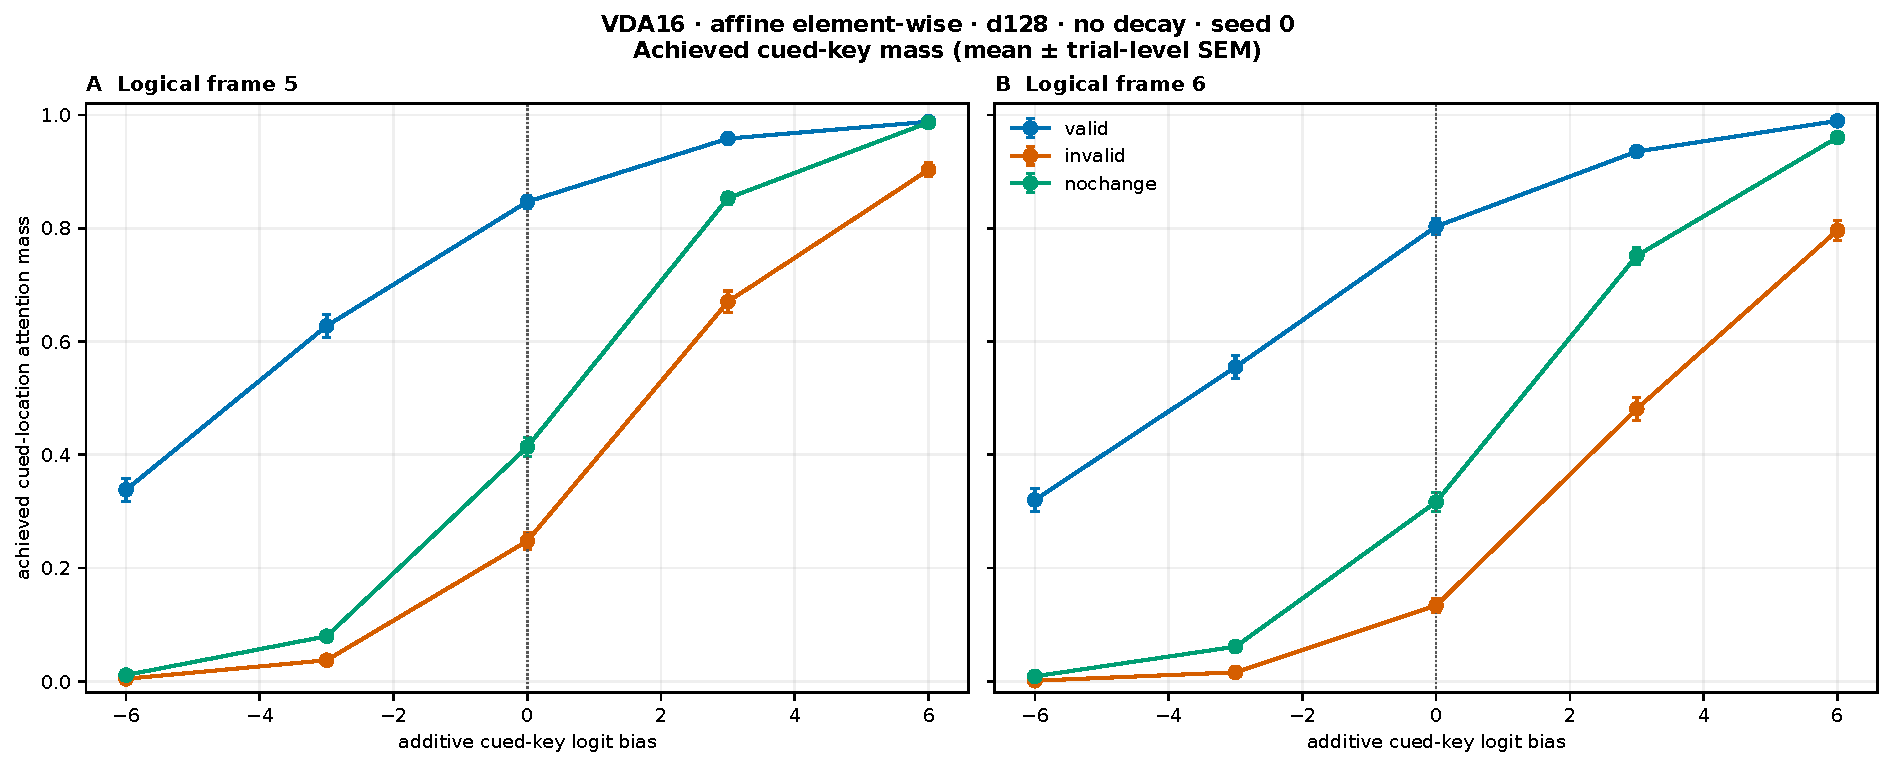
\includegraphics[width=0.49\textwidth]{vda16_affine_clamp_achieved_attention.pdf}
\caption{\textbf{Achieved cued-location attention mass under the additive bias sweep, cross-attention (left) and affine (right).} Both routing families' achieved attention rises smoothly with nominal bias; only affine's \emph{invalid-trial} sensitivity falls monotonically as that mass grows, because the boosted location is the wrong one on invalid trials.}\label{fig:vda16-clamp}
\end{figure*}

\subsection{The rescue test: biasing the true change location}\label{sec:pending-intervention}
The lever above always targets the location the cue points to, whether or not that location changes. Here we instead target the \emph{true change location on an invalid-cue trial} -- the condition that directly tests the Moore--Armstrong/Cavanaugh--Wurtz logic on this model. Section~\ref{sec:vda16-paired-attention} showed achieved frame-5 attention of 0.062 at the uncued change location versus 0.102 when that location was cued, alongside a behavioral gap from 0.983 to 0.490 qualifying response rate at the same focal magnitude. If that routing deficit is what \emph{causes} the behavioral deficit, restoring it by force should recover behavior, and removing it further should make an already-poor trial worse.

On trials with the change forced away from the cue (300 trials/condition, common random numbers, $30^\circ$ focal magnitude, cross-attention checkpoint), we sweep the identical graded bias independently at three locations: the true change location (the test itself), the cued-but-wrong location (negative control), and a fourth, task-irrelevant location (spatial-specificity control). All three reuse the primitives above with no new model code.

\textbf{Targeting the true change location produces the predicted double dissociation} (Figure~\ref{fig:change-loc}). Relative to the unbiased invalid-trial baseline ($51\%$ qualifying response rate, $d'=1.91$): full suppression collapses detection to \textbf{7\%} ($d'=0.38$); full boost recovers it to \textbf{95\%} ($d'=3.33$), closing \textbf{92\%} of the gap to the independently measured valid-trial ceiling of 98\%. Achieved attention at the true change location tracks this exactly -- suppression drives it to zero from the moment the bias switches on; boost drives it to 99\% by the response frame, against 33\% at baseline. Response timing among trials that do respond barely moves (5.5--6.0 frames throughout): \textbf{the intervention changes whether the model detects the change, not how quickly it responds once it does.}

Neither control location reproduces the rescue. Suppressing the cued-but-wrong location barely moves response rate ($51\%\to54\%$); boosting it instead \emph{lowers} response rate to $42\%$ and nearly quadruples the false-alarm rate ($3\%\to25\%$) -- a less stable, more trigger-happy policy, not improved detection. Suppressing the neutral location is similarly inert ($51\%\to53\%$); boosting it drops response rate to $9\%$, comparably severe to suppressing the true change location itself. Achieved attention at the true change location falls to 7\% (cued-boost) and 3\% (neutral-boost) of baseline, so the impairment reads as competitive -- forcing routing weight elsewhere pulls it away from where it is needed, rather than adding a generic, location-independent gain. \textbf{The rescue is spatially specific to the true change location. It is not an artifact of biasing attention anywhere.}

\begin{figure*}[t]
\centering
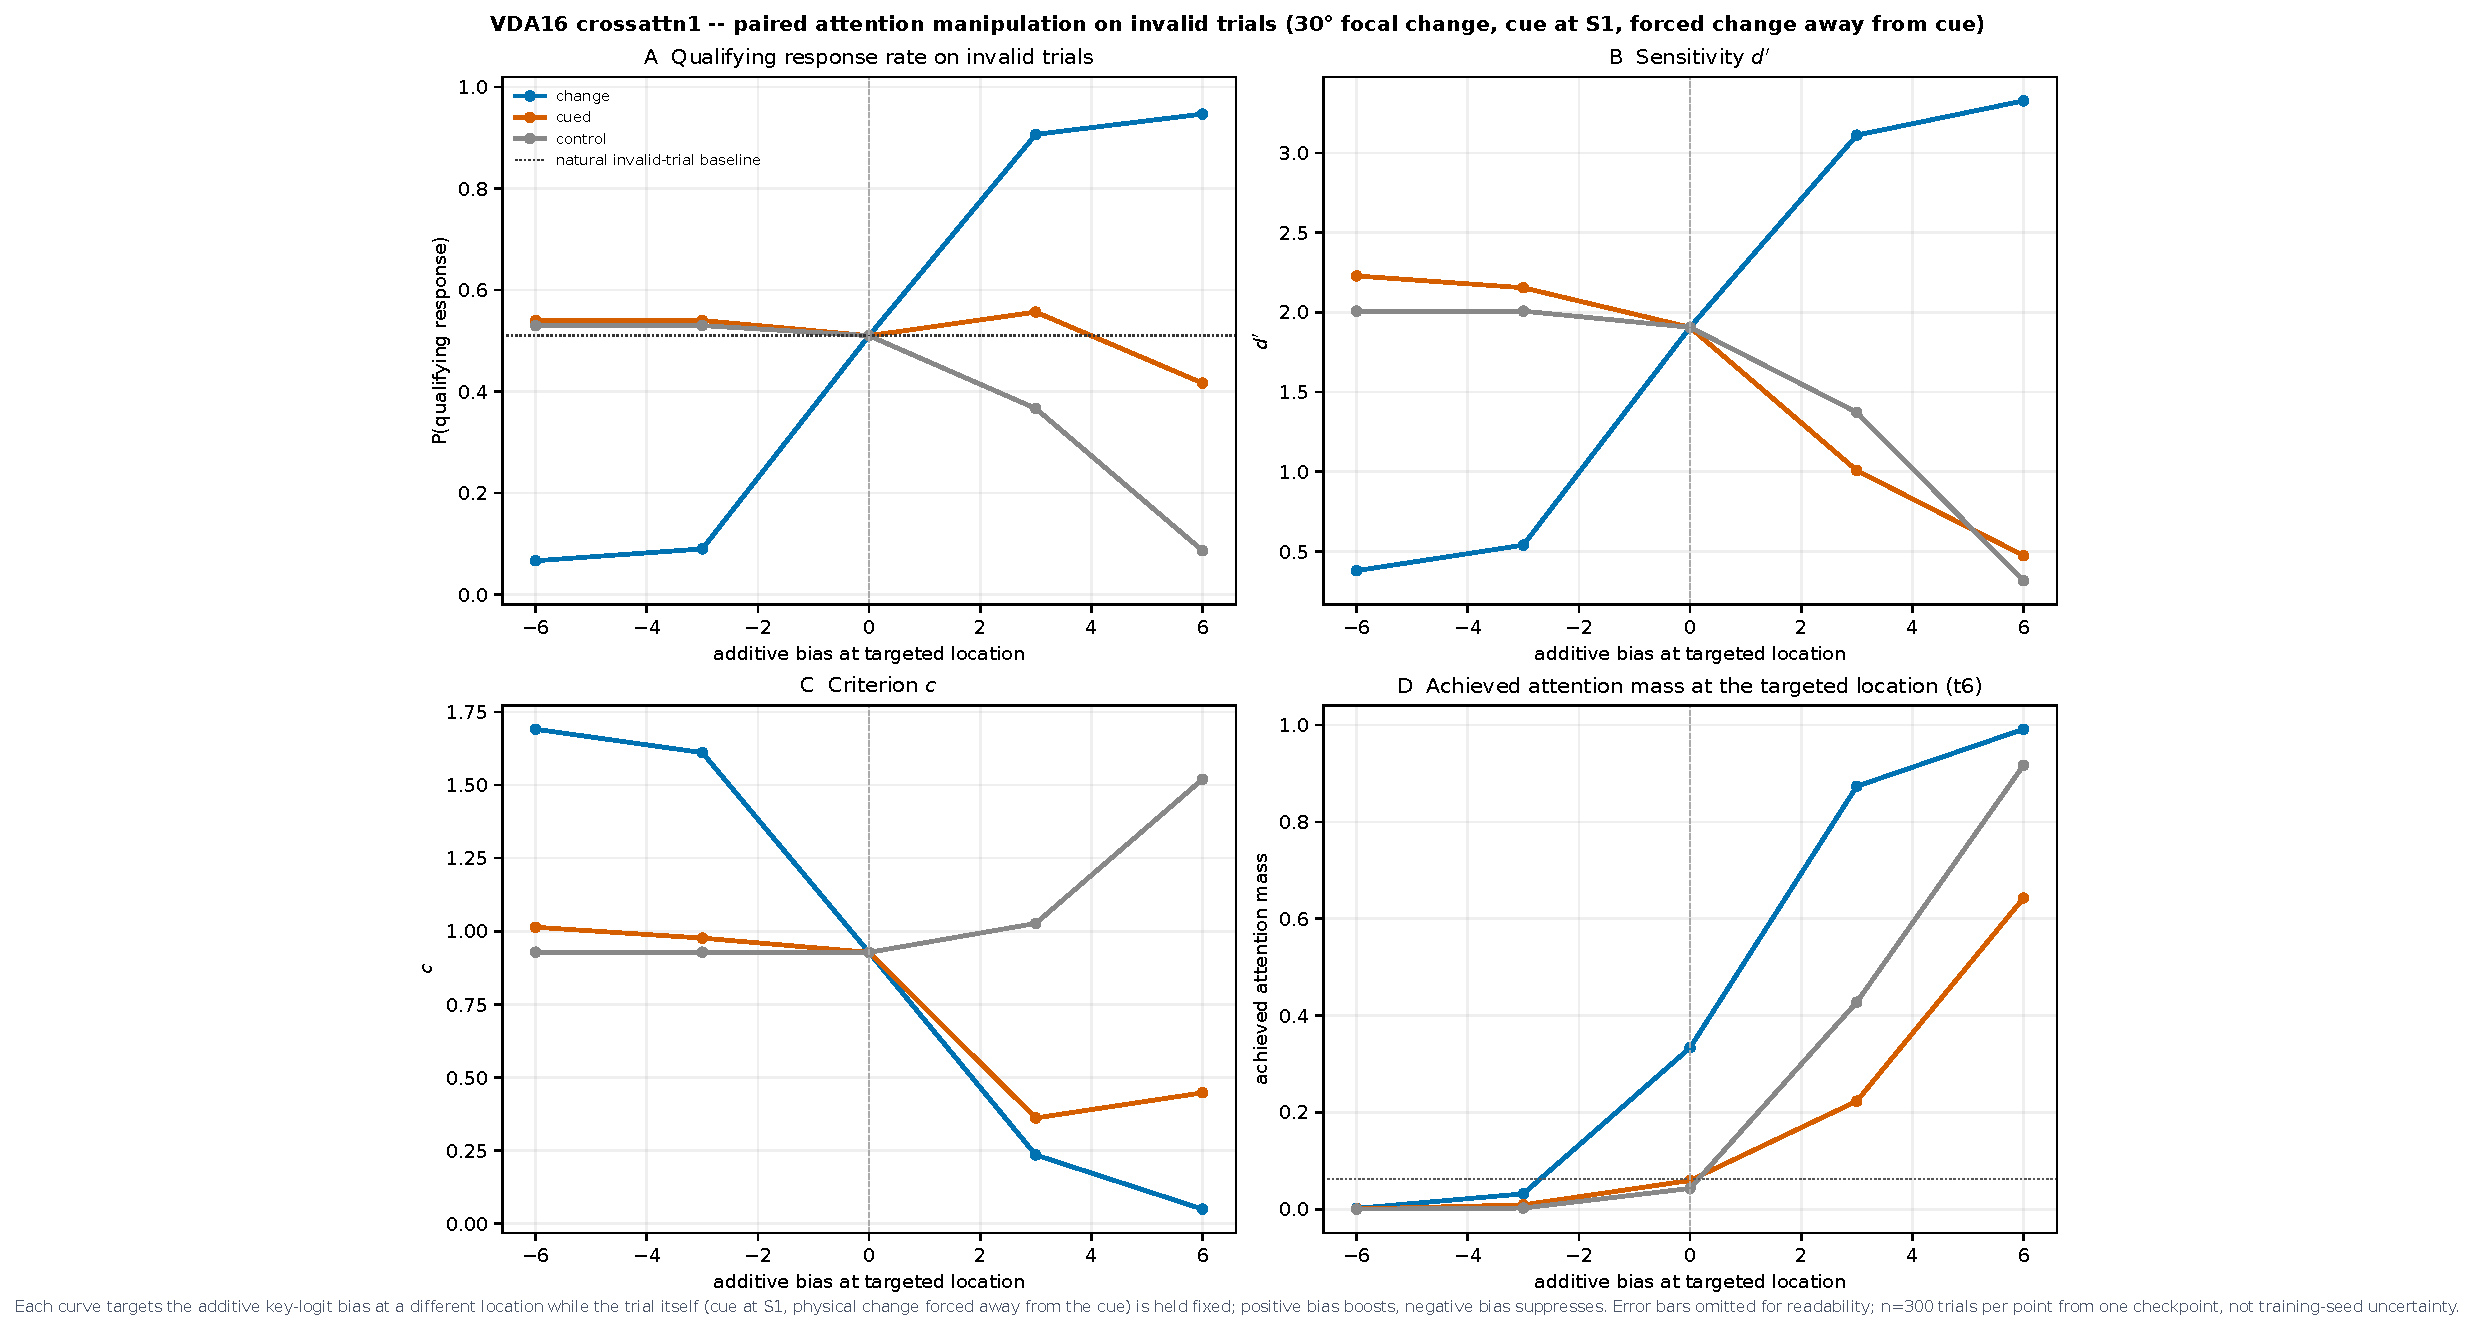
\includegraphics[width=0.85\textwidth]{vda16_change_location_intervention_summary.pdf}
\caption{\textbf{The central result of this paper: a spatially specific causal double dissociation.} On invalid-cue trials, the same graded bias is targeted independently at the true change location, the cued-but-wrong location, or a neutral location. (A) Qualifying response rate -- only the true-change-location curve rescues detection; the dotted line marks the unbiased baseline. (B) Sensitivity $d'$. (C) Criterion $c$. (D) Achieved attention at the targeted location. Cross-attention, VDA16, one competence-gated checkpoint, 300 trials/condition.}\label{fig:change-loc}
\end{figure*}

\begin{figure}[t]
\centering
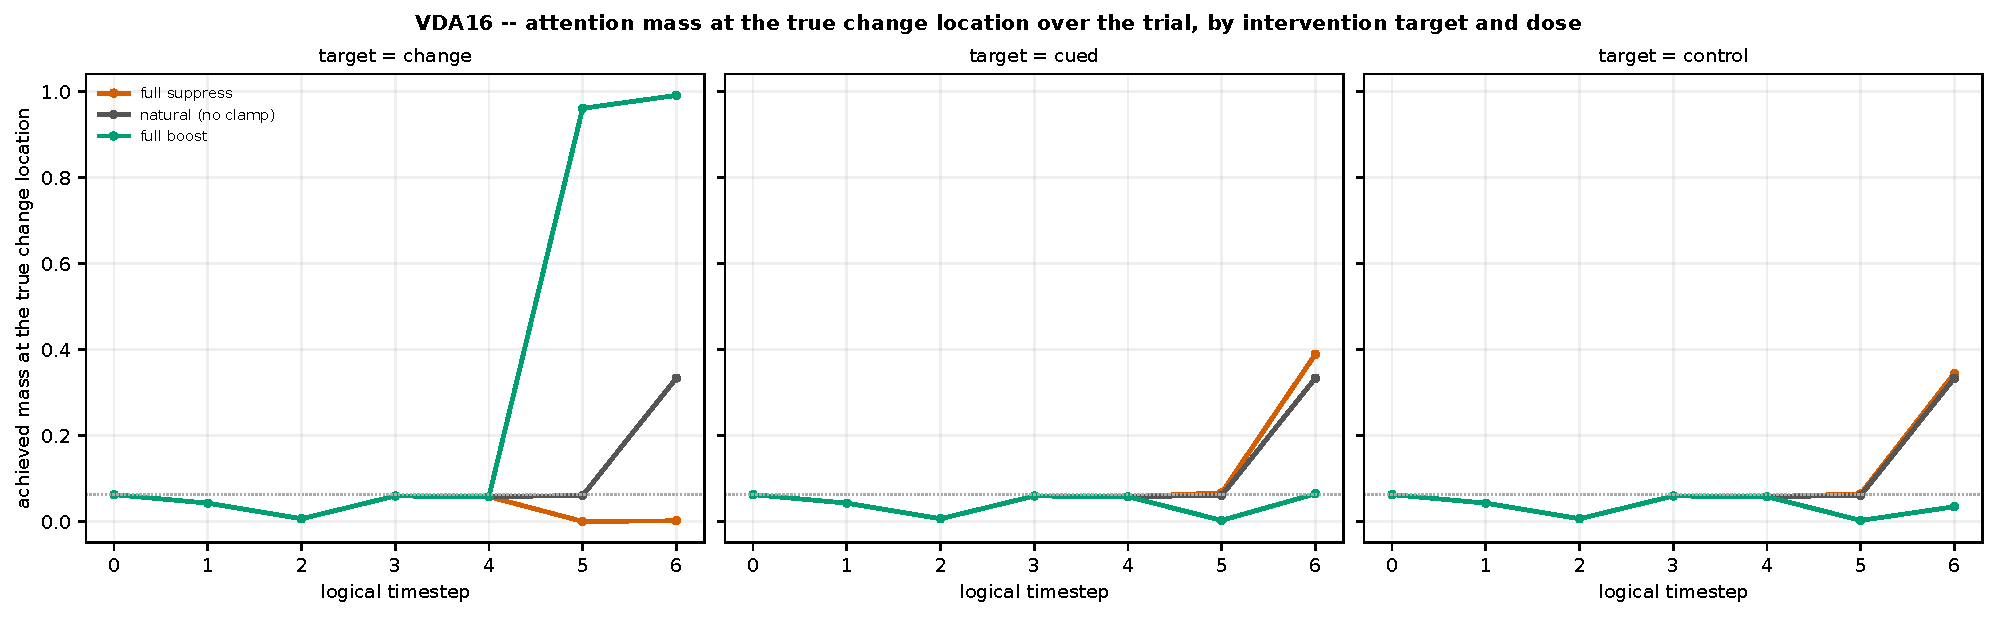
\includegraphics[width=\linewidth]{vda16_change_location_attention_trajectory.pdf}
\caption{\textbf{Achieved attention at the true change location across the full trial, by intervention target.} Only directly targeting the true change location moves its own achieved mass upward; boosting either control location competitively \emph{reduces} it below baseline instead.}\label{fig:change-loc-trajectory}
\end{figure}

\note{This is a single-checkpoint, finite-trial result on one competence-gated VDA16 seed. Within this checkpoint and intervention range, the bidirectional manipulation shows spatially specific, intervention-sensitive control associated with routing at the true change location rather than a generic gain change. It is a model-level counterpart to the Moore--Armstrong/Cavanaugh--Wurtz logic, not evidence of biological equivalence, architectural necessity, or seed-general sufficiency. The producer-bound bundle also still requires independent semantic verification. Whether the same dissociation holds at smaller set sizes is taken up next for VDA4 (VDA9 remains blocked by a missing checkpoint).}

\subsection{Does the rescue scale down? A fresh VDA4 checkpoint}\label{sec:vda4-rescue}
The gap above is now partly closed. A cross-attention, $d_{\mathrm{mem}}=128$ VDA4 checkpoint -- trained fresh for this test, same architecture and curriculum as every other checkpoint in this paper, reaching iteration 19{,}999 at $\theta=47^\circ$ (the same competence-gated floor status as the VDA16 checkpoints, not evidence of full convergence) -- lets us run the identical three-location battery at set size 4.

\textbf{The ordering replicates: targeting the true change location still produces the largest, most orderly effect of the three roles.} Relative to the unbiased invalid-trial baseline (42\% qualifying response rate, $d'=1.32$): suppression drops detection to \textbf{27\%} ($d'=0.90$); boost raises it to \textbf{59\%} ($d'=1.83$) -- a clean, monotonic dose-response with no analogue in either control condition (Figure~\ref{fig:vda4-change-loc}).

\textbf{But the effect is smaller and shaped differently than at VDA16.} Suppression here is a partial impairment, not the near-collapse to floor VDA16 showed ($27\%$ vs.\ VDA16's $7\%$). More strikingly, the cued-but-wrong-location control no longer behaves as a near-inert negative control: \emph{suppressing} it \emph{raises} response rate above baseline ($42\%\to51\%$), the opposite of VDA16's roughly flat pattern, while boosting it still hurts ($42\%\to30\%$), the same direction as VDA16. The false-alarm signature that made VDA16's wrong-location boost read as ``trigger-happy'' is also largely absent here (false-alarm rate moves only $6.3\%\to7.0\%$, not VDA16's $3\%\to25\%$). The task-irrelevant control location shows the smallest swing of the three roles ($42\%\to42\%$ suppress, $42\%\to34\%$ boost), consistent with genuine spatial specificity surviving the change in set size even where the finer details do not.

The two checkpoint-specific intervention curves differ. One possible explanation is softmax spillover: with four locations, weight removed from one location is redistributed over three alternatives rather than fifteen. That account is not isolated here, because VDA4 and VDA16 also differ in checkpoint, task scale, focal magnitude, native grid, and software stack. \textbf{Set size may change the shape of the causal intervention, but a monotonic set-size effect and the spillover mechanism remain hypotheses.} \note{One freshly trained, competence-gated VDA4 checkpoint, cross-attention only. This checkpoint was trained and evaluated on a different local software stack (PyTorch 2.8.0+cu128 vs.\ 1.13.1+cu117 for every other checkpoint in this paper) because the pinned version is not installable on the available hardware; behavior is expected, not guaranteed, to be unaffected by that difference. VDA9 remains blocked by a missing checkpoint.}

\begin{figure*}[t]
\centering
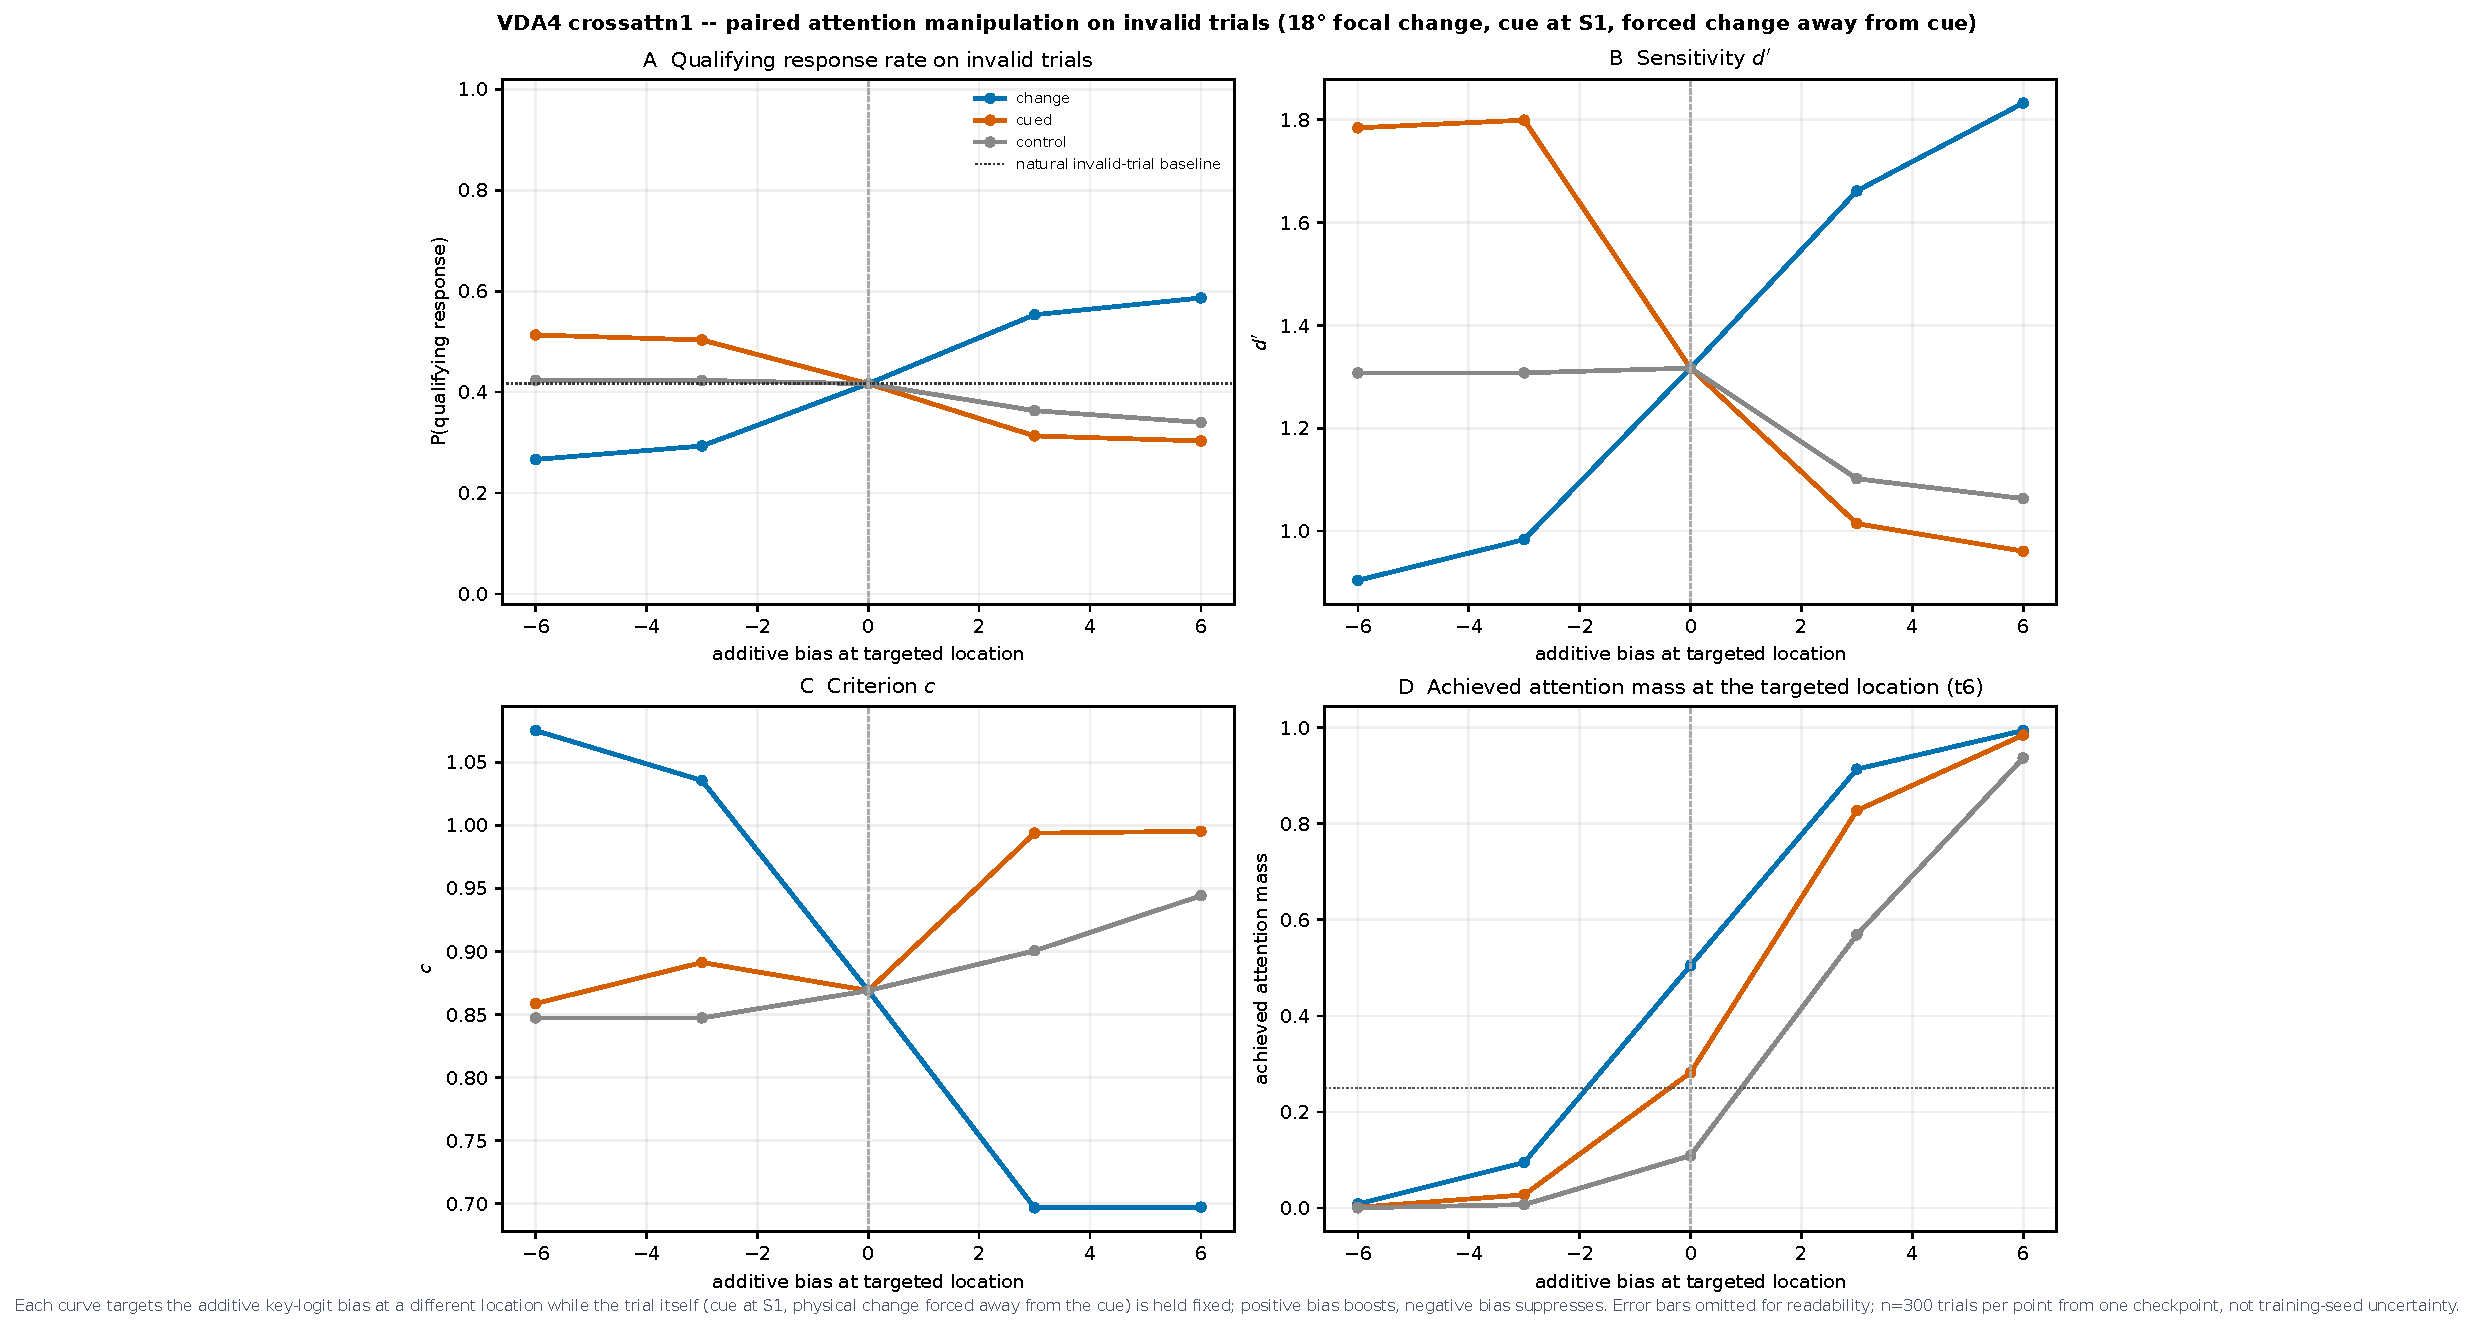
\includegraphics[width=0.85\textwidth]{vda4_change_location_intervention_summary.pdf}
\caption{\textbf{The same rescue test at set size 4.} Same design as Figure~\ref{fig:change-loc}: on invalid-cue trials, the graded bias targets the true change location, the cued-but-wrong location, or a task-irrelevant location. The true-change-location curve (blue) still shows the largest, most orderly dose-response, but suppressing the cued-but-wrong location now \emph{raises} response rate above baseline instead of leaving it flat, unlike at VDA16. Cross-attention, VDA4, one freshly trained checkpoint, 300 trials/condition.}\label{fig:vda4-change-loc}
\end{figure*}

\FloatBarrier
\section{Discussion: Attention as Signal Coherence}\label{sec:discussion}
\textbf{The organizing hypothesis is functional: attention increases signal coherence.} In this model, that means that cue- and target-consistent visual and memory signals become spatially aligned, persist through the relevant delay and event, separate from competing alternatives, and reach the decision policy in usable form. This definition deliberately spans routing, representation, behavior, and causal use. More concentrated routing is one possible mechanism, not a sufficient endpoint; a larger cueing gap can reflect stronger selection, weaker invalid-location sensitivity, or a criterion shift.

\textbf{The strongest current producer-bound result is checkpoint-local, spatially specific response causality.} It would have been entirely possible for routing to correlate with the cue and behavior without doing causal work. In the evaluated competence-gated VDA16 cross-attention checkpoint, suppressing the correctly identified location sharply impairs detection and boosting it recovers 92\% of the valid-cue ceiling, while wrong- and neutral-location operations do not reproduce the rescue. That double dissociation is consistent with target-signal propagation at this checkpoint; it remains provisional until independently semantically verified and does not establish every representational component of the coherence theory or population generality.

\textbf{Routing stability covaries with recurrent-memory persistence.} In the evaluated VDA4 checkpoint pair, the higher-decay checkpoint has greater frame-to-frame routing variation. Because the decay arms are separately trained and represented by one seed each, this is an architectural covariation rather than evidence that forgetting causes unstable attention or that attention and memory are inseparable. It remains a specific, falsifiable echo of persistent-activity accounts of working-memory maintenance \cite{luck1997,awh2001}.

\textbf{Object competition and patch-level competition are distinct predictions.} The historical cross-attention lineage shows a monotonic behavioral cueing increase from 4 to 16 active items, consistent with selection becoming more consequential when more objects compete; affine rises and then plateaus. The fixed-task experiment instead adds patches while holding four active objects constant. Its premise is that finer sampling creates more non-target routing alternatives and therefore increases the need to propagate the target signal. The existing results constrain the simplest version: cross-attention seed 0 loses valid-target frame-5 concentration, affine peak-quadrant share remains high, and the second cross-attention seed reverses the valid endpoint direction. The seed-0 response-rate disable effect grows sharply only for affine and declines for cross-attention; cross-attention behavioral and sensitivity-corrected directions do not replicate. Thus the right question is not whether ``attention increases with tokens,'' but whether normalized routing, target representation, sensitivity, and spatially specific causal leverage increase together as patch competition grows.

\textbf{The coherence account has explicit failure conditions.} Its simple discretization prediction is unsupported if an apparent effect exists only in raw peaks with a $1/N$ baseline; disappears for equal-area or uniform-normalized measures; changes criterion without improving sensitivity or utility; produces a sharper map without a stronger target representation or behavioral consequence; is equally sensitive to true, wrong, and neutral interventions; appears only at the post-decision frame 6; or reverses across adequately replicated training seeds. Conversely, the strongest support would be a preregistered $N\times$ cue-validity and $N\times$ intervention-location interaction at frame 5, accompanied by a stronger held-out target-code margin and sensitivity-corrected behavior under fixed parameters and common trials.

\textbf{What remains open.} The six-cell native-grid control changes token count, native support, attention cardinality, readout size, and parameter count together. The registered fixed-100-carrier visual-by-memory stream factorial is the next binding test because it varies effective visual streams $V\in\{4,100\}$ and memory streams $M\in\{4,100\}$ without changing the carrier; it remains incomplete and has no admitted held-out attention or causal results, so it contributes no claim here. Completing it can test whether visual and memory signal rank interact and whether a rank-preserving cyclic misbinding selectively impairs, then restoration rescues, routing, representation, and sensitivity. Because all 100 carrier positions remain in the softmax, this factorial does \emph{not} test native key-cardinality competition. That requires a separate fixed-parameter manipulation with 4, 16, or 100 eligible or independently varying spatial alternatives while carrier and readout shapes remain fixed; merely broadcasting 4/16 grouped values over 100 keys tests signal rank, not competitor count. A complementary fixed-carrier $K\in\{4,9,16\}$ experiment is needed for the active-item claim. Cross-attention endpoint replication presently covers only two seeds; the midpoint, all affine cells, and inferential training-population uncertainty remain unreplicated. Future caches must preserve trial-level image- and memory-source mass and query-region--key-region structure. Multi-seed designs with disjoint calibration/evaluation banks, non-saturated change magnitudes, and identical trial streams are required to estimate the predicted interactions. The rescue test has a VDA4 data point (Section~\ref{sec:vda4-rescue}), but VDA9 remains blocked. Sensitivity/criterion decomposition covers both VDA16 checkpoints but not the first-wave VDA4/VDA9 or width-comparison psychometrics.

\note{The admissible language throughout this paper is ``model-level counterpart,'' ``structurally analogous,'' or ``corresponds to.'' No result here identifies a routing tensor as FEF, SC, LPFC, or biological working memory, and none of it establishes population-level precision or human/primate capacity. The only training-seed replication is the $n=2$ cross-attention endpoint comparison; it does not support population generality.}

\FloatBarrier
\section{Methods and Reproducibility}\label{sec:methods}
Every quantitative or causal claim above traces to an explicit checkpoint and cached analysis artifact; provenance detail that would otherwise interrupt the narrative is summarized here rather than boxed beside every figure. Historical aggregates come from a preserved NPZ archive with no producer hash or per-point trial count and are never treated as more than a qualitative landscape. The first-wave, matched-width, and VDA16 batteries instead execute exact, hash-verified checkpoints after freezing source bytes, write immutable trial-level and reduced caches, and pass an independent read-only provenance audit; the matched-width battery's review returned \emph{approve with limits} (separate-checkpoint, finite-trial, and competence-gate limits remain explicitly active). VDA16's cross-attention checkpoint is competence-gated at curriculum angle $\theta=65^\circ$ (never advanced from initialization); its affine counterpart advanced further to $\theta=47^\circ$ after a statefully resumed training run recovered by saved checkpoint hashes; neither reached the declared $8^\circ$ floor. The change-location intervention (Section~\ref{sec:pending-intervention}) is produced by a new, independently written script (\texttt{change\_location\_intervention.py}) that reuses the existing, already-tested additive key-logit bias, forced-location trial generation, and signal-detection primitives rather than introducing new model code; its VDA4 arm now runs on a freshly trained checkpoint (Section~\ref{sec:vda4-rescue}), trained and evaluated on a different, documented software stack from the rest of this paper; its VDA9 arm remains recorded as explicitly blocked, with a manifest, rather than silently omitted. The cross-attention VDA16 and VDA4 rescue bundles have producer manifests but no separate semantic-verifier artifacts, so they are treated as provisional producer-bound checkpoint evidence; the independently verified affine VDA16 rescue remains a bounded single-checkpoint result near ceiling and does not verify the cross-attention effect. The logistic-fit re-analysis in Section~\ref{sec:psychometric-fits} performs no checkpoint or model access at all, only re-reading already-cached, already-verified response-probability arrays. The repository regression suite covers cache and checkpoint identity, matched stimulus generation, decoder chance levels, and competence gating; every page of the compiled manuscript is rendered and visually inspected. Appendix~\ref{app:provenance} lists every artifact's path and provenance class; the coverage matrices in Appendices~\ref{app:coverage}--\ref{app:disposition} record, cell by cell, which of the 952 source-derived panel--environment estimands are complete, available, blocked, undefined, or inapplicable, so that absence of evidence is always a recorded, explained state rather than a silent gap.

The spatial-scaling battery in Section~\ref{sec:discretization-test} is a separate production lineage. Completion requires trainer exit, exactly contiguous finite metrics for iterations 0--19{,}999, terminal final/latest checkpoints, schema/config/provenance validation, clean final-save logs, and independently matched local/remote SHA-256 values. Each admitted checkpoint then runs the same held-out evaluator at 300 psychometric, 128 attention, and 250 intervention trials per condition. The newly completed affine $2\times2$ checkpoint has SHA-256 \texttt{2db6c8a6...3314197} (full value in the production manifest); its 13 declared evaluation artifacts passed 1{,}347 independent integrity and semantic checks with no failures. The endpoint replication adds fresh seed-1 cross-attention checkpoints at $2\times2$ and $10\times10$; the new $2\times2$ terminal checkpoint has SHA-256 \texttt{31c498bd...0a59}, 20{,}000 contiguous finite rows, semantically equal final/latest state, all 15 producer/config/launcher hashes verified remotely and locally, and a complete 13-artifact held-out evaluation (manifest SHA-256 \texttt{054c7bac...2703}). The four-source endpoint synthesis consumes only the two grids at seeds 0 and 1. Its independent read-only verifier checked 52 source artifacts and 66 total hashes, recomputed all reported endpoint metrics, completed 2{,}246 semantic checks, and decoded 26 source and bundle figures (bundle manifest SHA-256 \texttt{3c0acd3b...8ddb}). The seed-0 six-cell synthesis and the endpoint synthesis both read only verified evaluation caches; no training metric is used as attention evidence.

The attention-measure re-analysis first reads the eight admitted \texttt{event\_attention.npz} caches only after matching each cache to its source manifest SHA-256. It reconstructs and internally cross-checks the legacy paired-location patch-column scores, verifies equality with cached trial-level patch mass, and applies the exact common-$2\times2$ partition. Because those admitted caches had retained cross-attention source identity only after trial averaging, a focused source refresh replays only the same 128 valid and 128 forced-invalid event trials from each of the five hash-matched terminal cross-attention checkpoints. It stores visual- and recurrent-memory-source mass before addition, verifies exact press-array equality, and reconstructs the admitted paired-location arrays within maximum absolute error $7.1\times10^{-9}$ to $3.0\times10^{-8}$ across the five checkpoints. No retraining, psychometric rerun, or intervention rerun enters that refresh. The derived bundle writes 6{,}144 legacy paired-location/affine trial rows, 7{,}680 source-resolved trial rows, 864 legacy summaries, 1{,}500 source summaries, paired grid contrasts using common trial IDs, twelve explicit metric definitions, and eleven vector figures under \path{spatial_scaling_attention_measures_20260803_source_separated_v6/}. Percentile intervals use 10{,}000 paired or within-cell trial-bootstrap draws. No training metric, curriculum value, checkpoint trajectory, or GPU/process diagnostic enters this attention analysis.

\FloatBarrier
\section{Conclusion}
We frame value-directed attention as a mechanism for increasing signal coherence: cue- and target-consistent visual and memory signals should become more spatially aligned, more decodable, more behaviorally useful, and more causally actionable relative to competing locations. The paper's strongest current producer-bound result is the checkpoint-local intervention: in one competence-gated VDA16 cross-attention checkpoint, true-location suppression sharply impairs detection and boost recovers 92\% of the valid-cue ceiling, while a plausible-but-wrong location does not reproduce the rescue; independent semantic verification and seed replication remain required. The active-item series supplies a motivating cross-attention pattern in which the cueing benefit grows from set size 4 to 16, but affine routing plateaus and the checkpoints are not a parameter-matched population series. The fixed four-item 4/16/100-token experiment then asks the sharper question: does finer image discretization create enough spatial-key competition that attention becomes more extreme and more behaviorally consequential even when set size is unchanged? Its answer is not yet monotonic. Total quadrant allocation, normalized peak concentration, event timing, source share, behavior, and causal dependence dissociate, and limited cross-attention seed replication reverses several directions. The coherence hypothesis is therefore explicit and falsifiable rather than declared proven: it requires convergence of equal-area normalized routing at the decision-relevant frame, target representation, sensitivity-corrected behavior, and spatially specific intervention under parameter-matched, replicated manipulations. Completing the fixed-carrier visual-by-memory binding factorial, separately varying eligible spatial competitors, and running a fixed-carrier active-item series are the decisive next tests. None of these findings licenses a claim about human or primate capacity, and no routing tensor is claimed to be a specific brain region; they are model-level counterparts with their evidentiary boundaries stated beside each claim.

\bibliographystyle{plain}
\begin{thebibliography}{9}
\small
\bibitem{mah2025} J.~Morgan, L.~Albanna, and J.~P.~Herman. Recurrent vision transformers model visual attention through feedback. \emph{arXiv:2502.10955v1}, 2025.
\bibitem{carrasco2011} M.~Carrasco. Visual attention: the past 25 years. \emph{Vision Research}, 2011.
\bibitem{herman2017} J.~P.~Herman and R.~J.~Krauzlis. Color-change detection activity in the primate superior colliculus. \emph{eNeuro}, 2017.
\bibitem{luo2018} T.~Z.~Luo and J.~H.~R.~Maunsell. Attentional changes in either criterion or sensitivity are associated with robust modulations in lateral prefrontal cortex. \emph{Neuron}, 2018.
\bibitem{moore2003} T.~Moore and K.~M.~Armstrong. Selective gating of visual signals by microstimulation of frontal cortex. \emph{Nature}, 2003.
\bibitem{cavanaugh2004} J.~Cavanaugh and R.~H.~Wurtz. Subcortical modulation of attention counters change blindness. \emph{Journal of Neuroscience}, 2004.
\bibitem{luck1997} S.~J.~Luck and E.~K.~Vogel. The capacity of visual working memory for features and conjunctions. \emph{Nature}, 1997.
\bibitem{awh2001} E.~Awh and J.~Jonides. Overlapping mechanisms of attention and spatial working memory. \emph{Trends in Cognitive Sciences}, 2001.
\bibitem{panichello2021} M.~F.~Panichello and T.~J.~Buschman. Shared mechanisms underlie the control of working memory and attention. \emph{Nature}, 2021.
\end{thebibliography}

\onecolumn
\appendix
\FloatBarrier
\section{Reference Material}
The results above are the paper; this appendix is the evidence trail behind them, kept in full because a claim this reliant on provenance (single checkpoints, hash-verified caches, explicit blocked/undefined states) should remain auditable. It is reference material, not required reading.

\subsection{Fourteen-environment task atlas}
\begin{center}
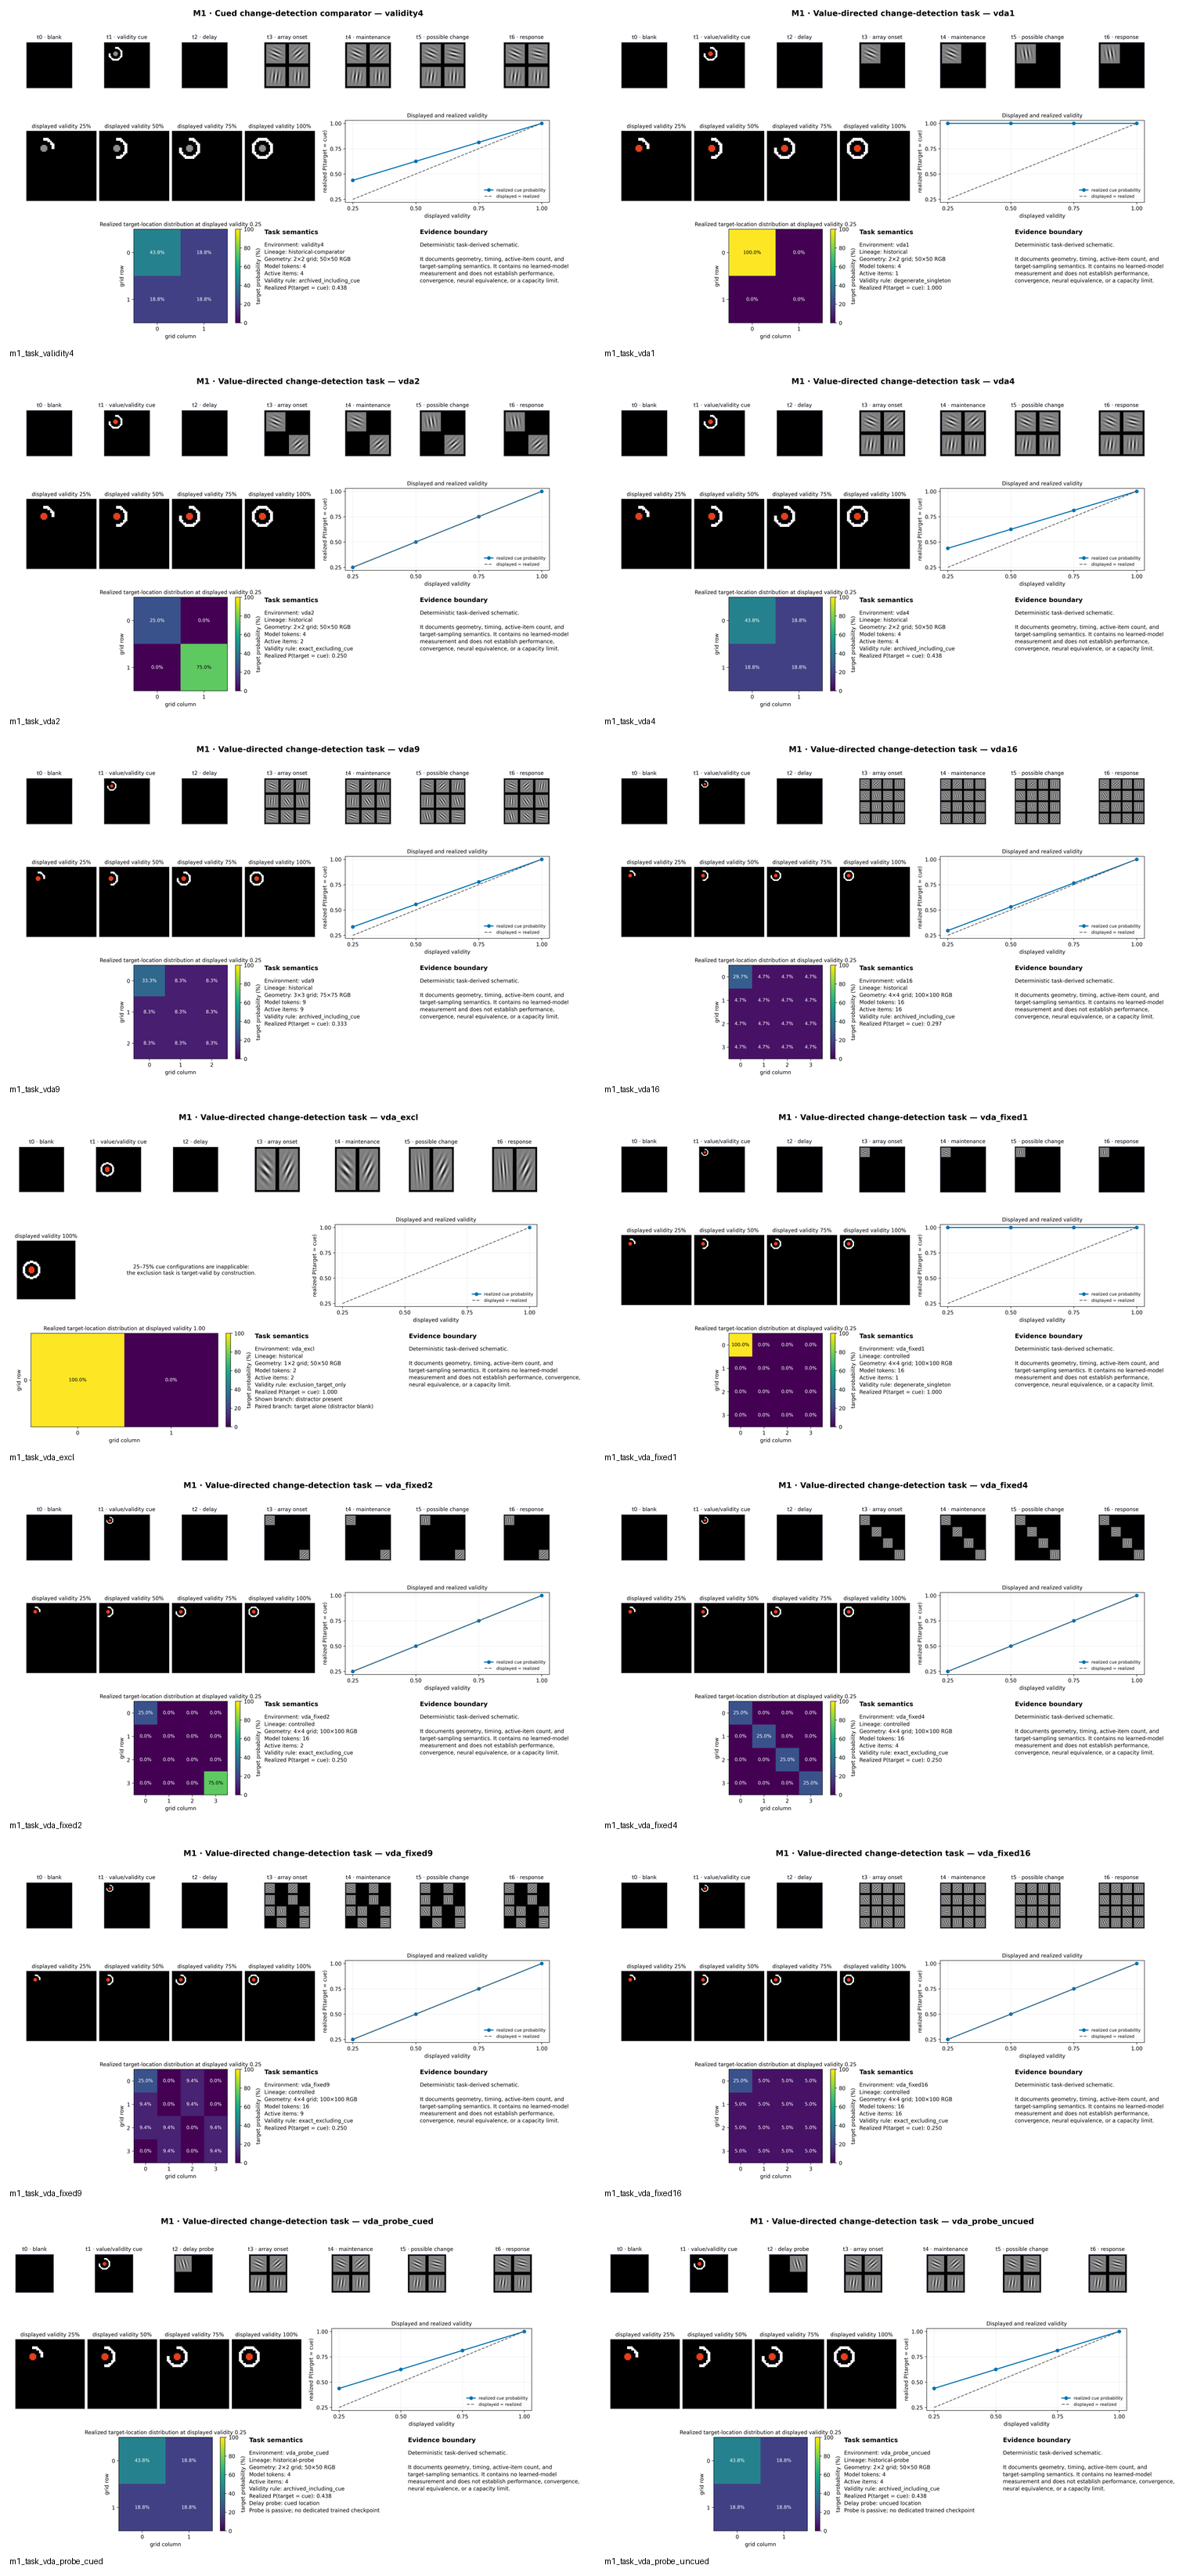
\includegraphics[width=0.72\textwidth,height=0.85\textheight,keepaspectratio]{m1_task_contact_sheet.png}
\end{center}
\captionof{figure}{All fourteen registered environments' deterministic task schematics, for cross-environment comparison. Left to right, top to bottom: neutral-validity comparator; historical VDA1/2/4/9/16; the exclusion task; cued and uncued delay probes; controlled fixed-grid VDA1/2/4/9/16.}\label{fig:m1-atlas}

\subsection{Full historical aggregate plates}\label{app:m3-full}
The eight plates behind Figure~\ref{fig:m3-overview}, regenerated from the preserved aggregate archive (checkpoints not rerun). VDA1's uncued-location panels (B, C, E, F) are omitted because a singleton has no uncued comparator.

\begin{center}
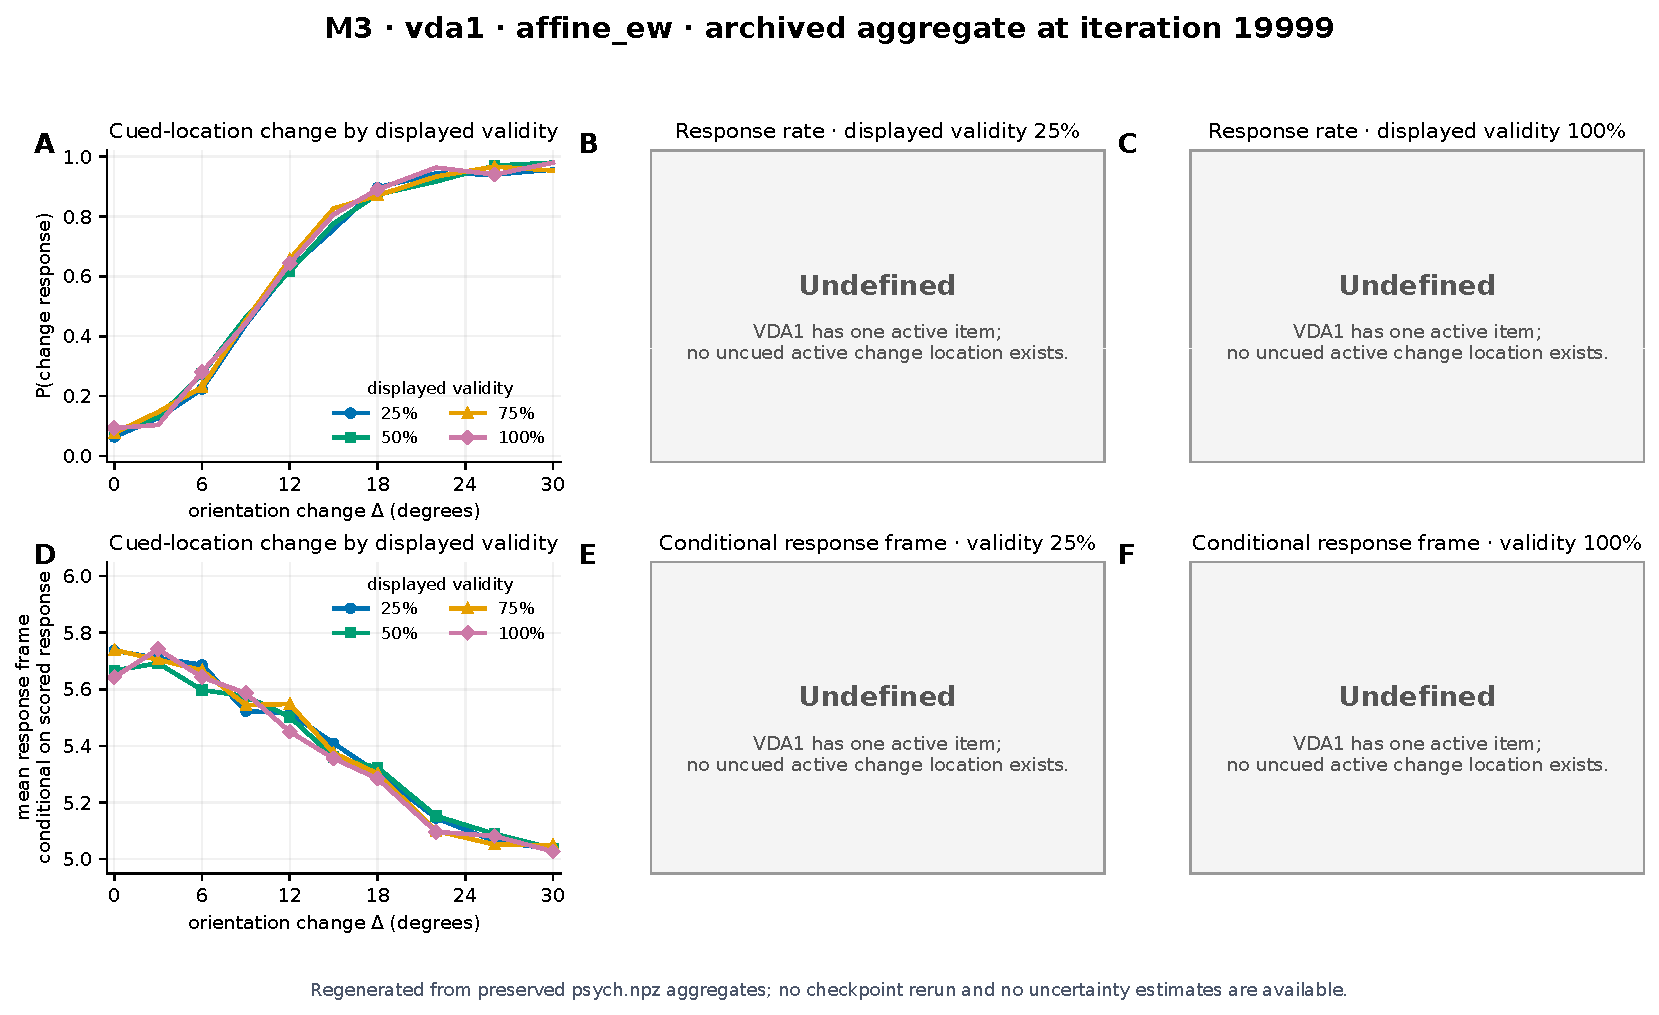
\includegraphics[width=0.44\textwidth]{m3_behavior_vda1_affine_ew.pdf}\hfill
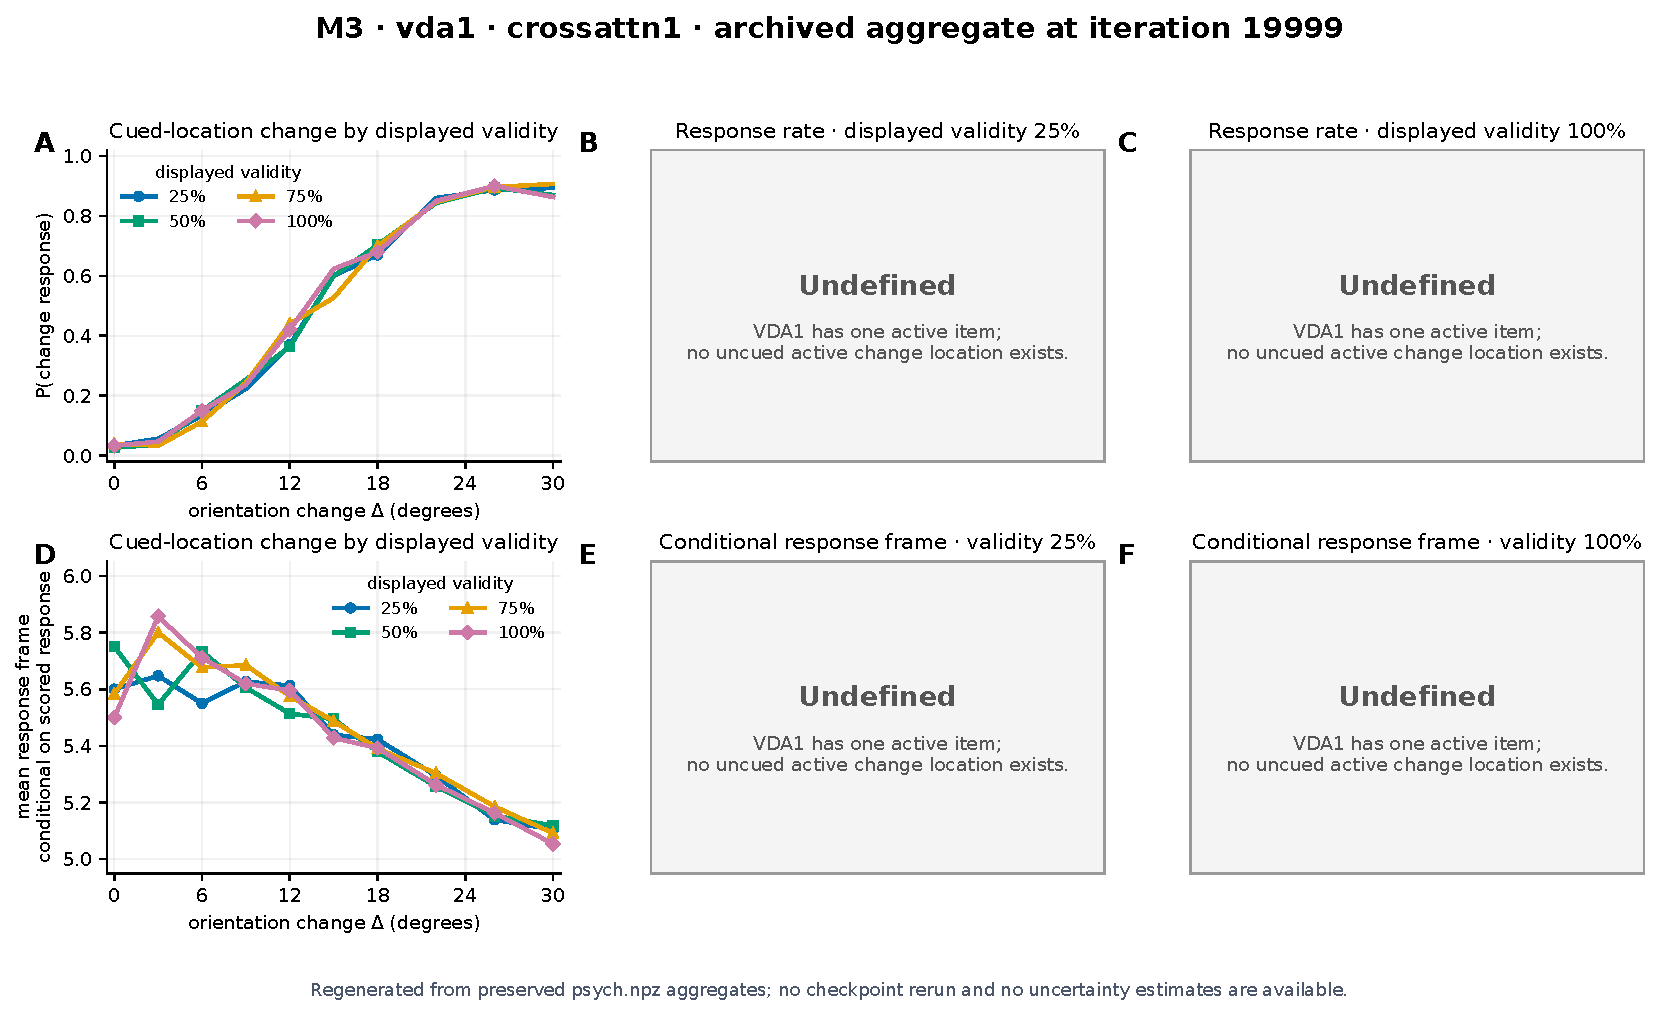
\includegraphics[width=0.44\textwidth]{m3_behavior_vda1_crossattn1.pdf}\\[3pt]
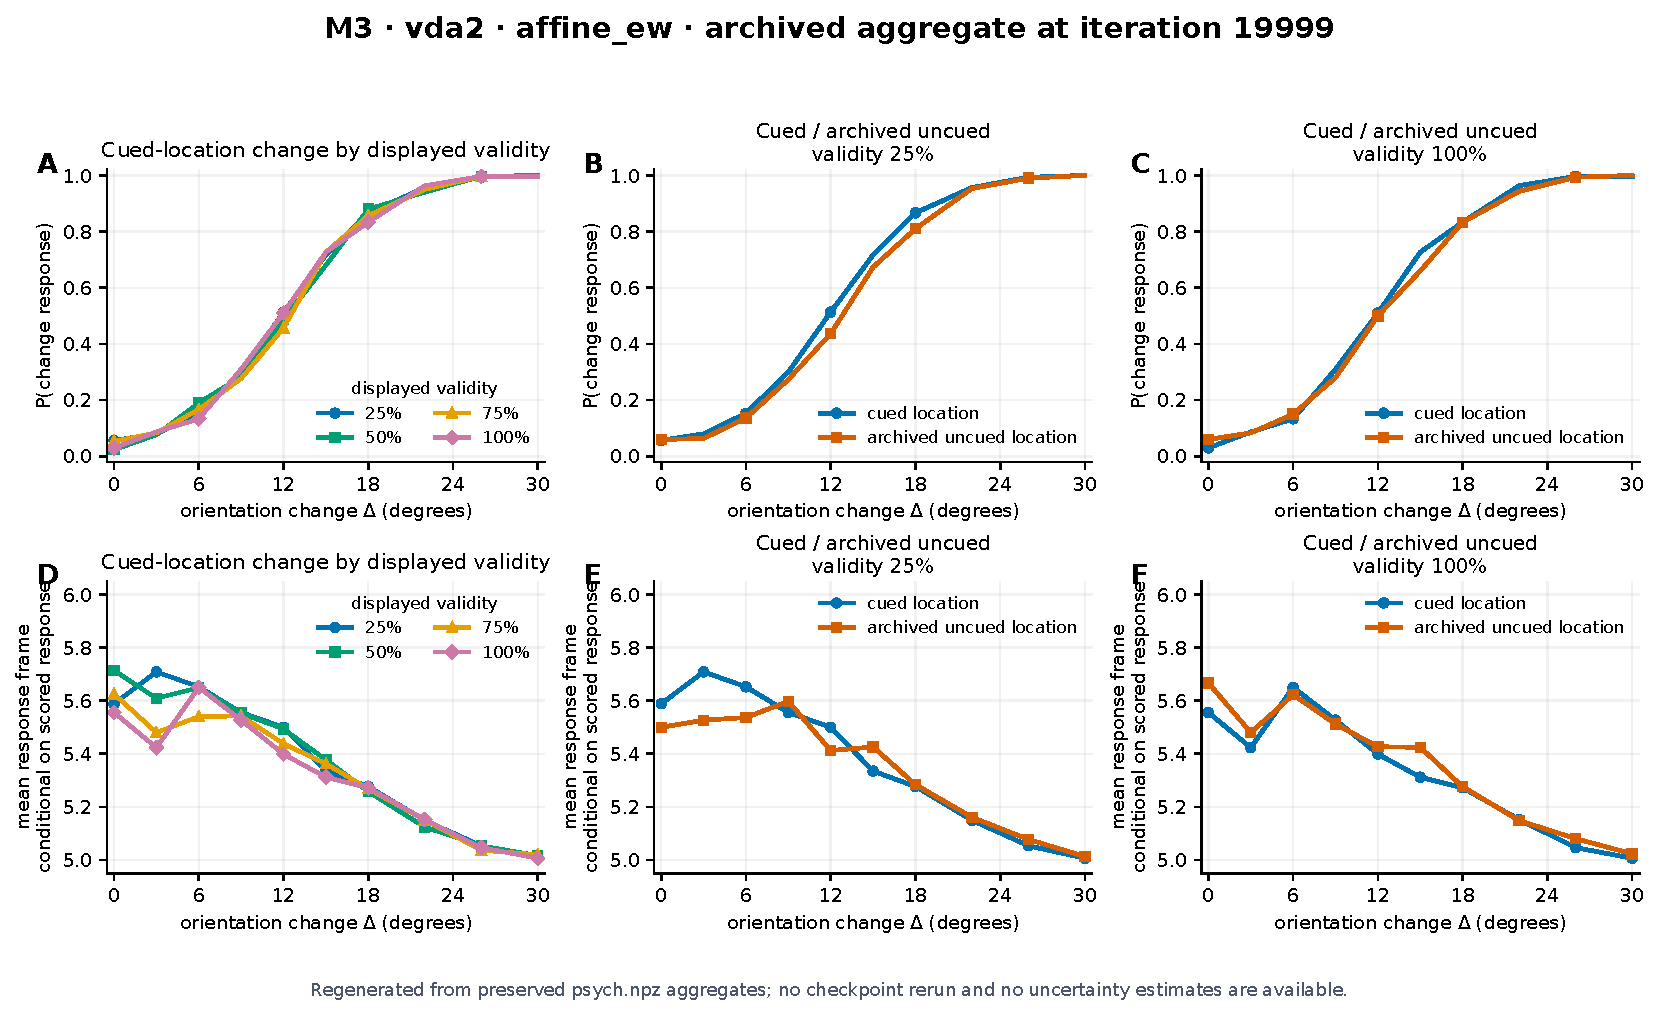
\includegraphics[width=0.44\textwidth]{m3_behavior_vda2_affine_ew.pdf}\hfill
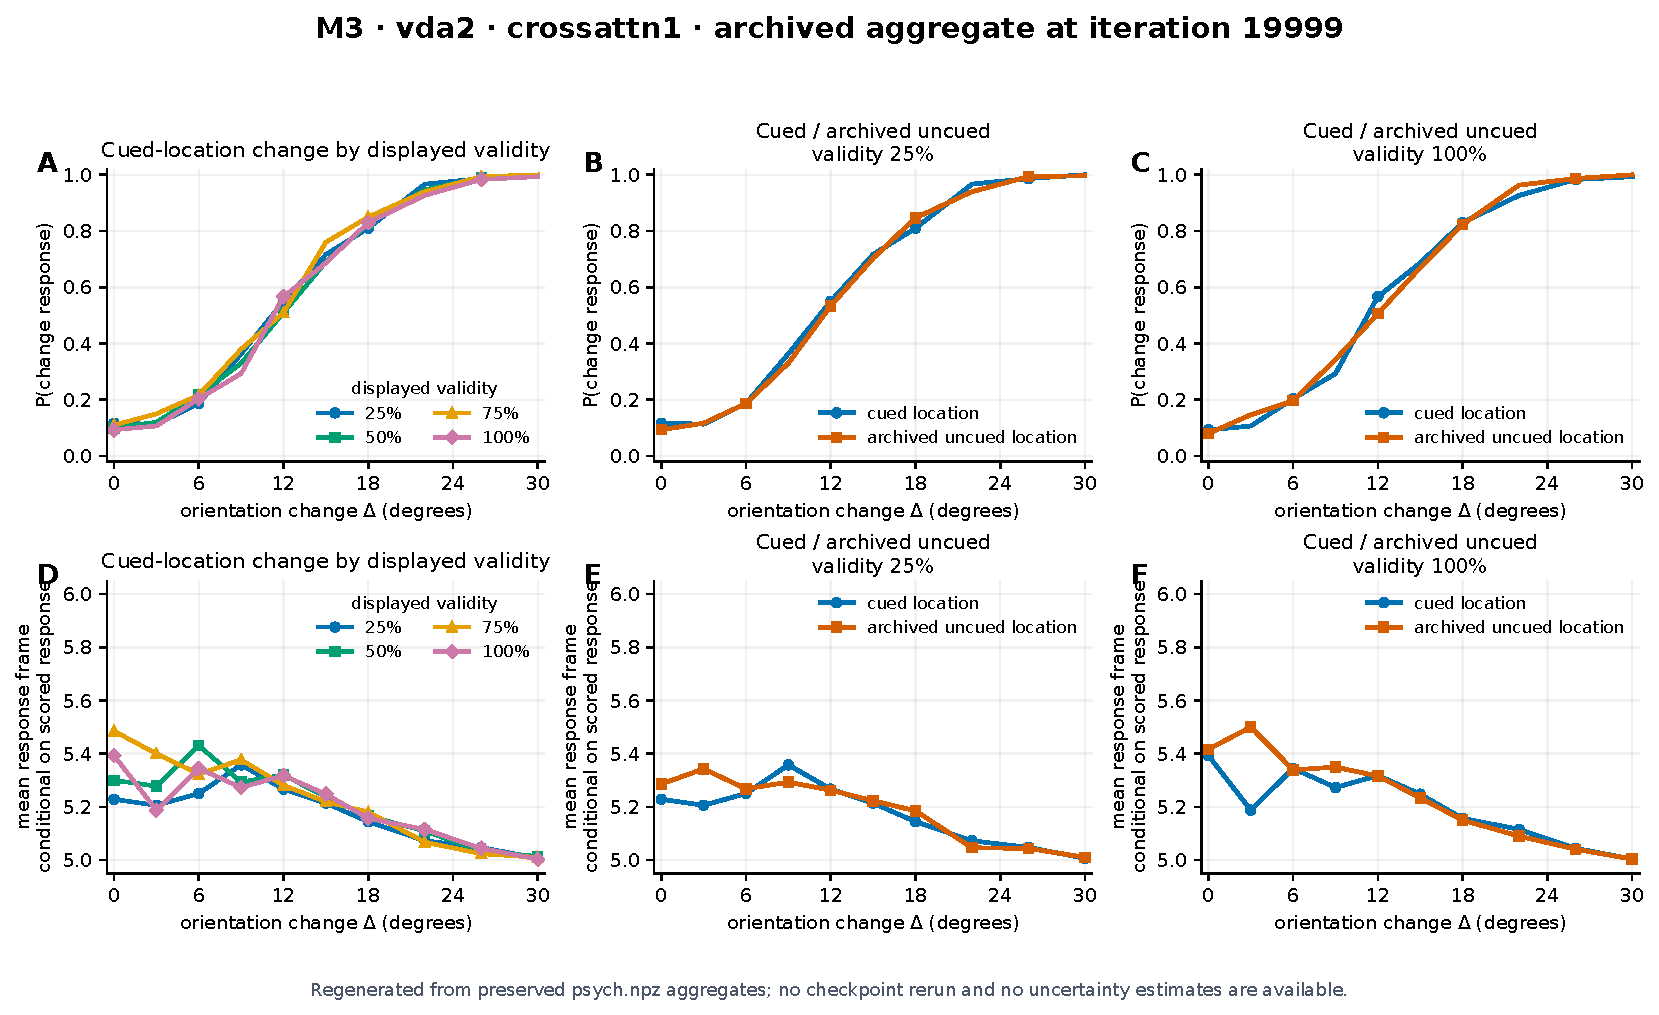
\includegraphics[width=0.44\textwidth]{m3_behavior_vda2_crossattn1.pdf}\\[3pt]
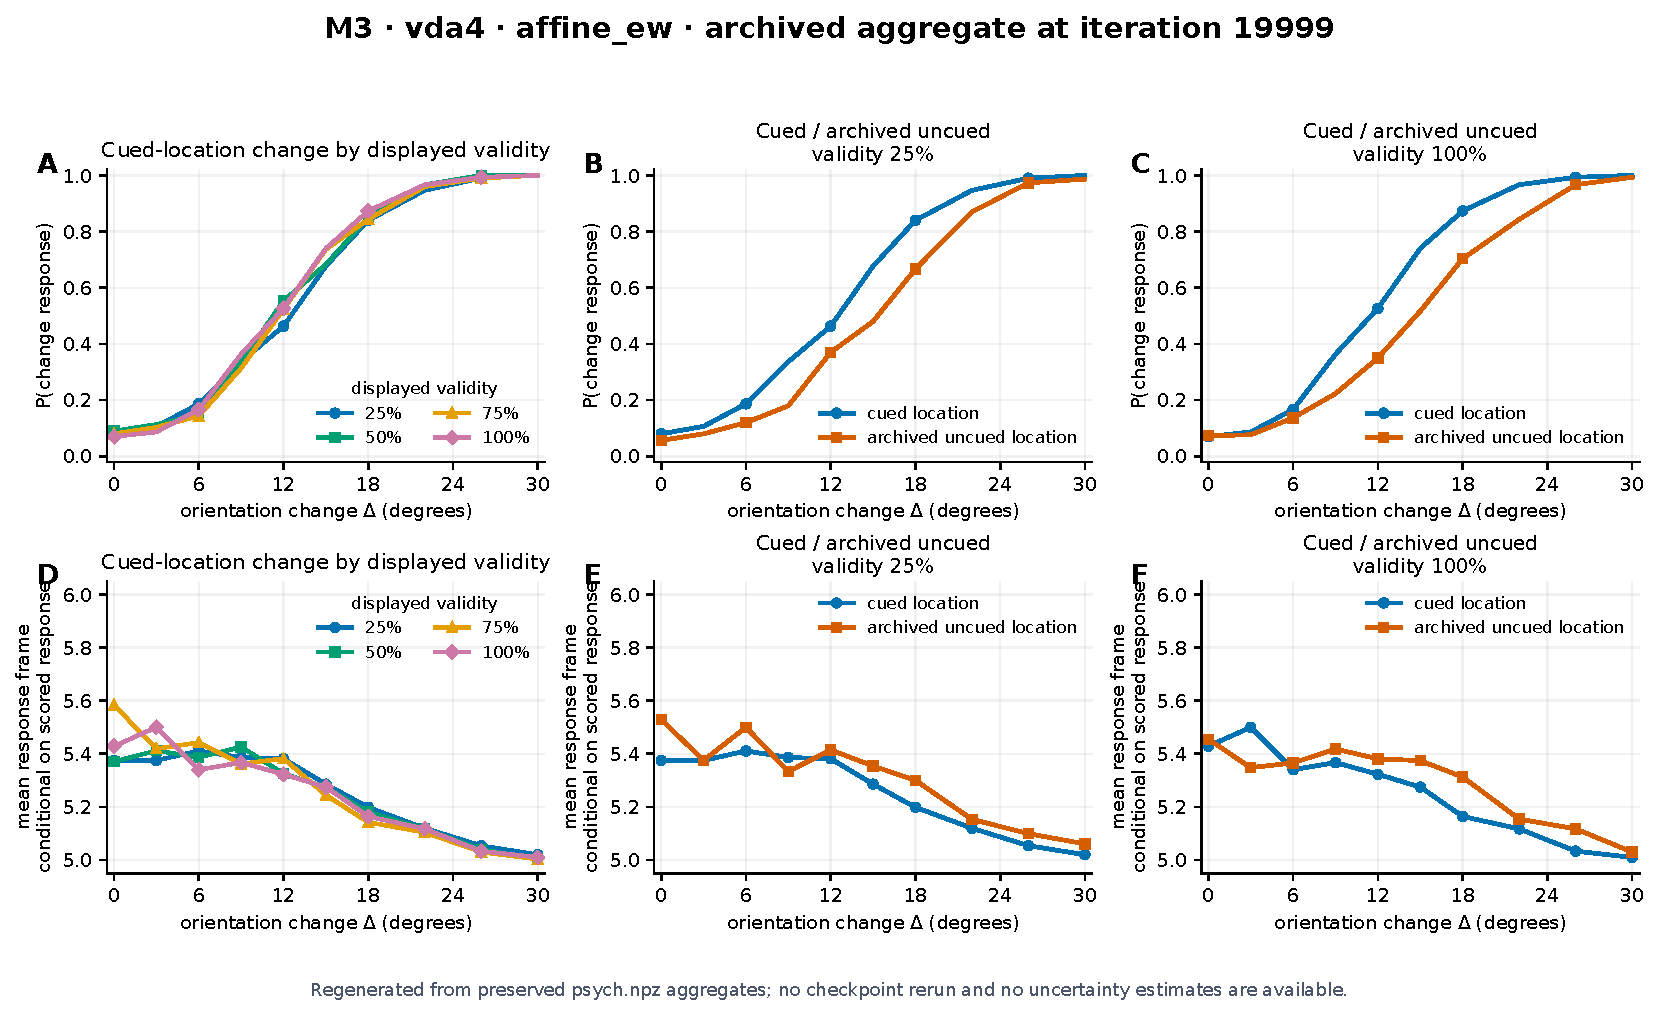
\includegraphics[width=0.44\textwidth]{m3_behavior_vda4_affine_ew.pdf}\hfill
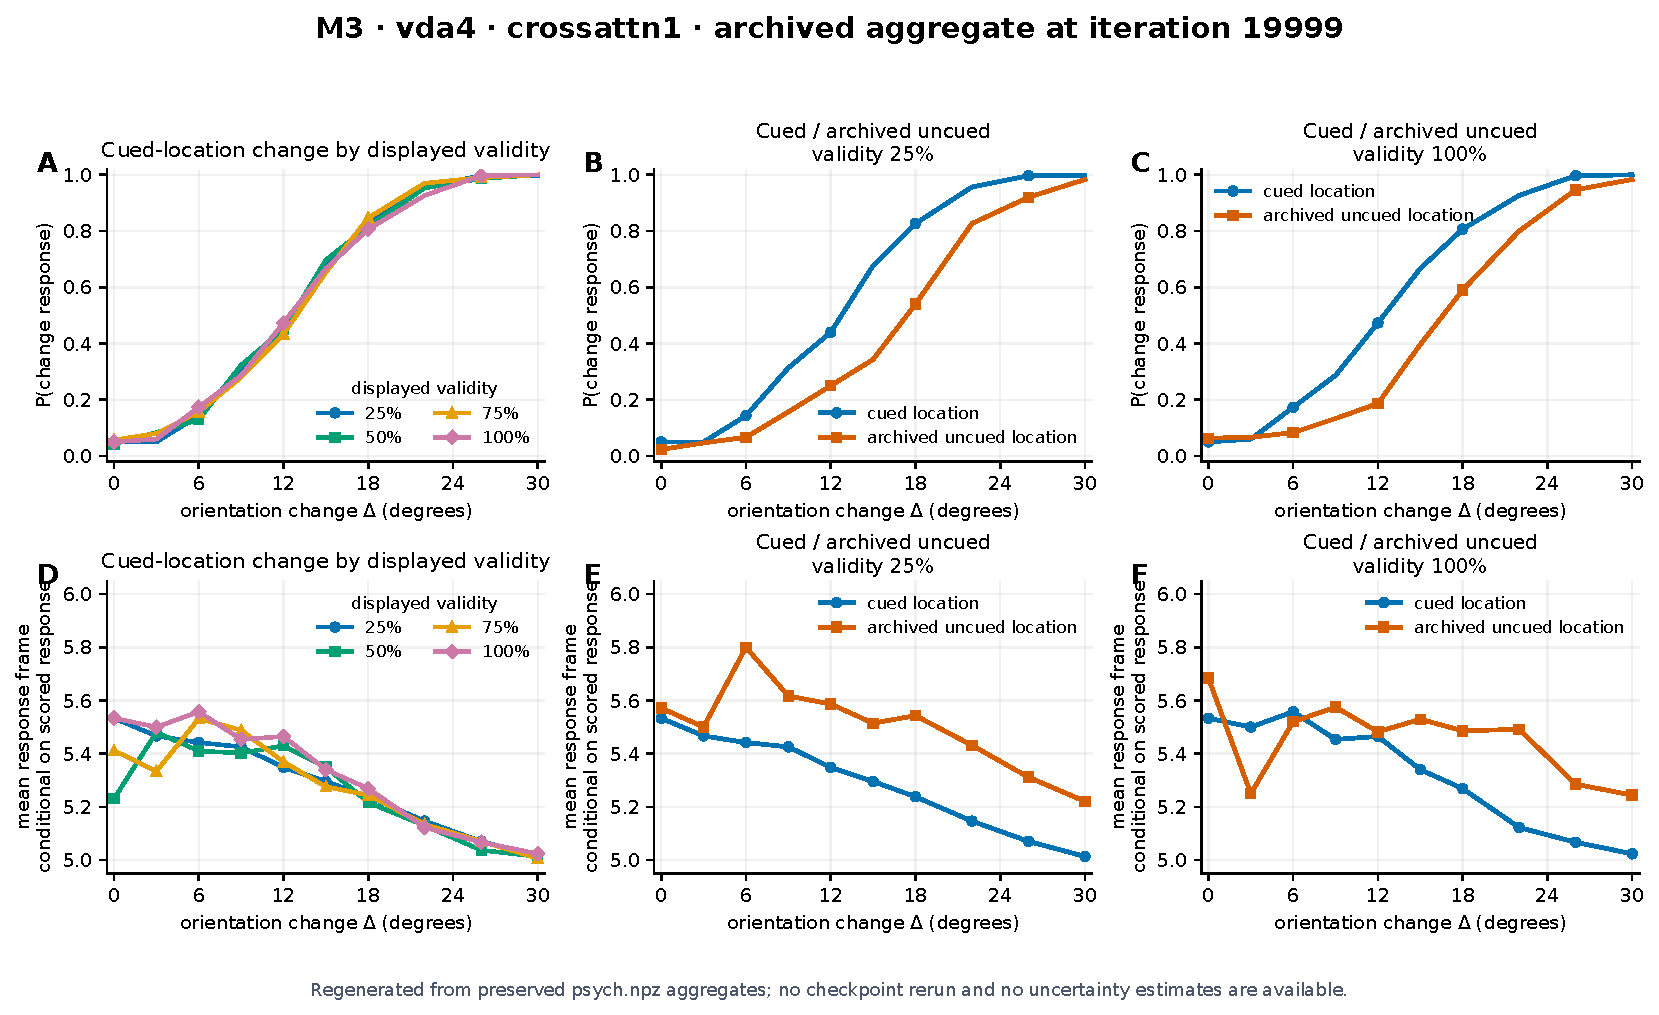
\includegraphics[width=0.44\textwidth]{m3_behavior_vda4_crossattn1.pdf}\\[3pt]
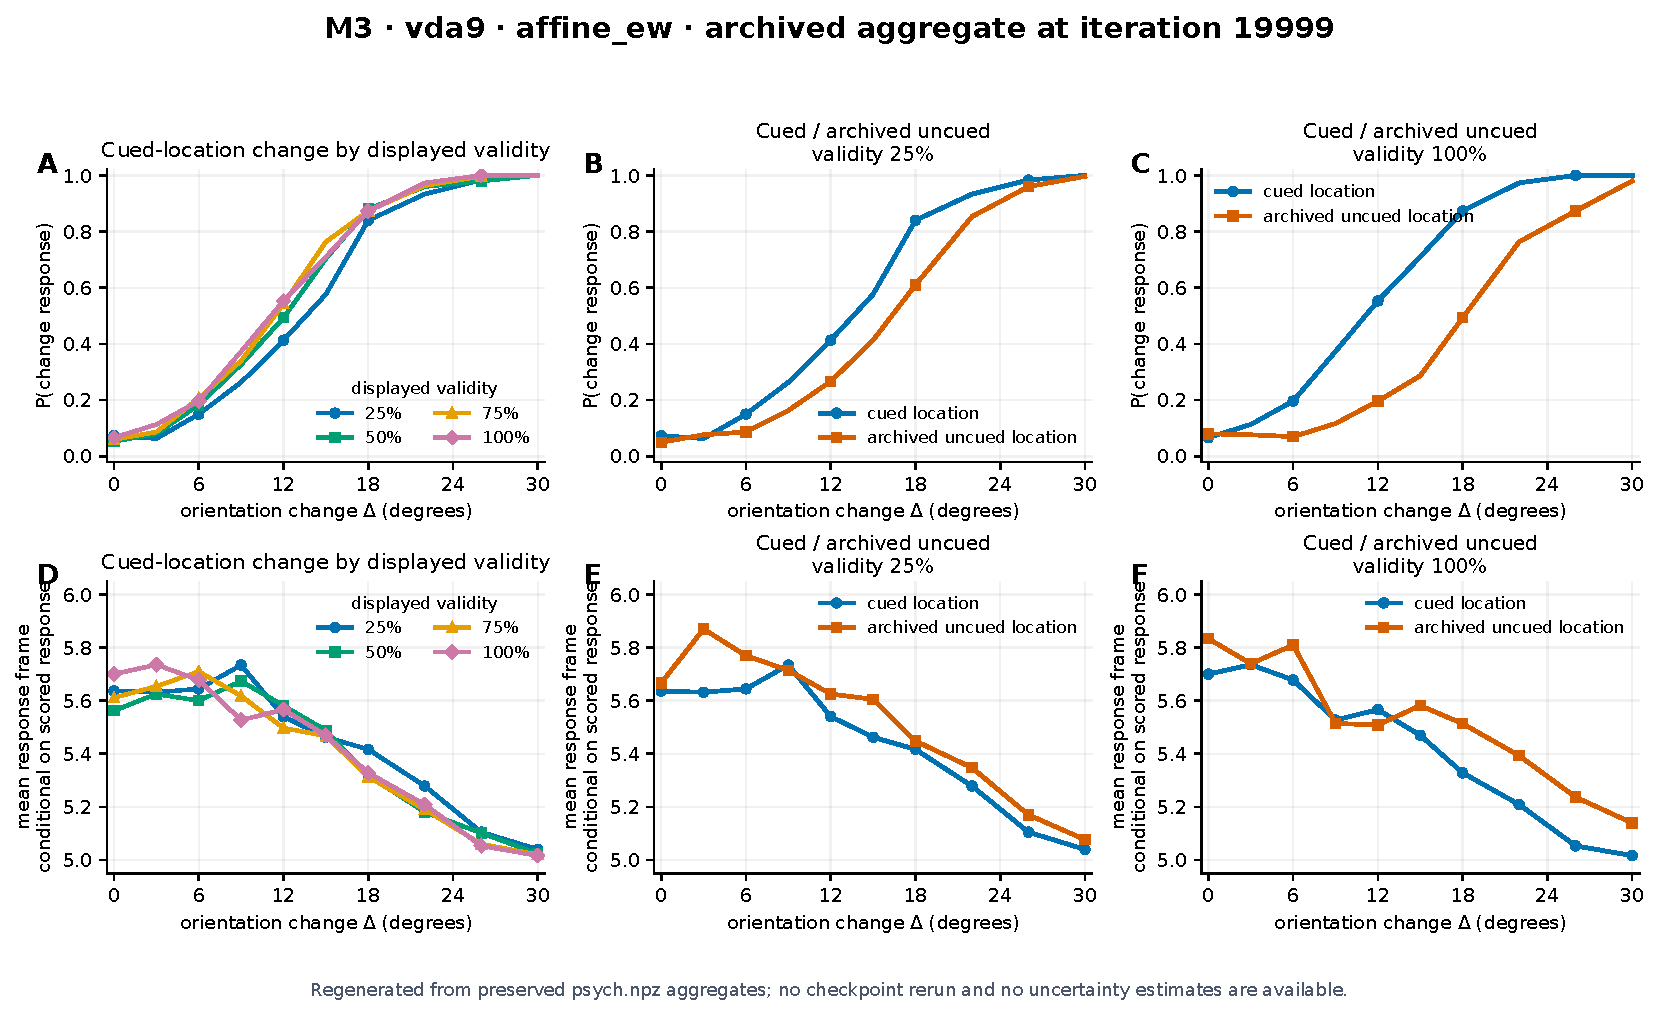
\includegraphics[width=0.44\textwidth]{m3_behavior_vda9_affine_ew.pdf}\hfill
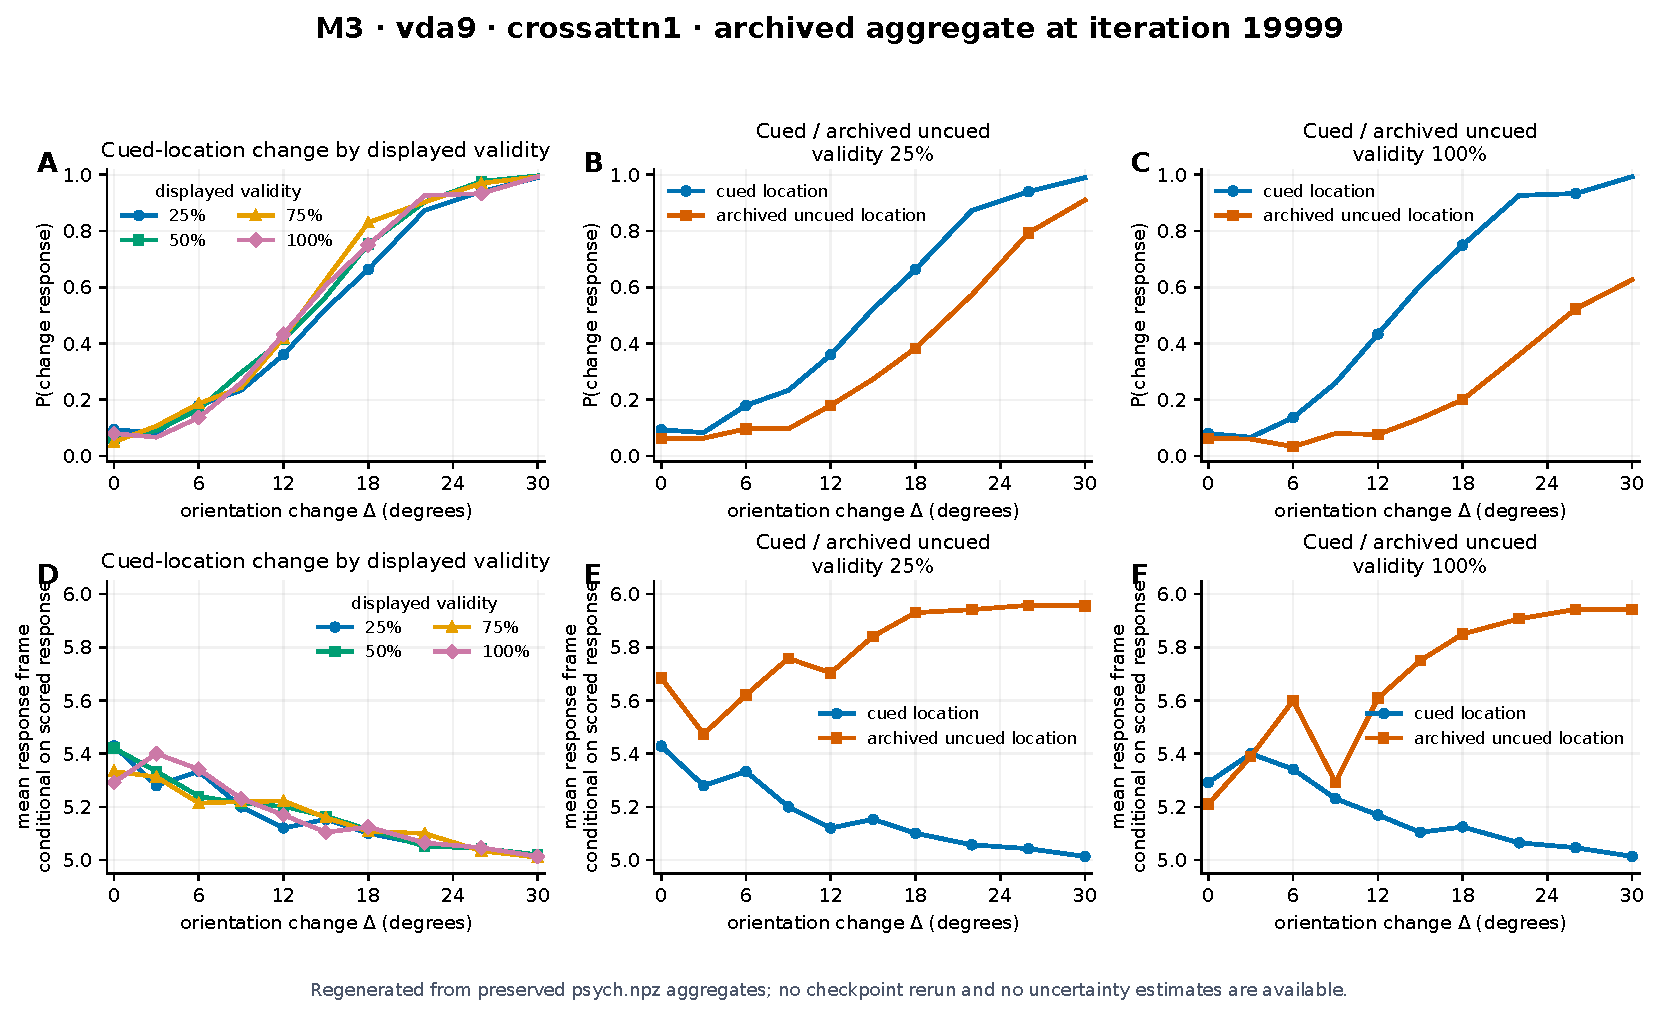
\includegraphics[width=0.44\textwidth]{m3_behavior_vda9_crossattn1.pdf}
\end{center}
\captionof{figure}{Rows: VDA1, VDA2, VDA4, VDA9. Columns: affine, cross-attention. Each panel labeled with its own routing family and environment in-figure.}

\clearpage
\subsection{Common-grid attention atlas}\label{app:attention-atlas}
These panels are alternative views of the verified held-out event bank used in Section~\ref{sec:discretization-test}; they are not training diagnostics. The first two retain the older paired-location $V+M$ diagnostic for cross-attention and label it as such. The remaining panels implement the established source-separated convention: visual and recurrent-memory keys remain distinct, use shared raw scales, and are followed through all seven frames. Source-resolved trial arrays were regenerated from the same hash-matched terminal checkpoints and common-random-number trials solely to retain the source axis before reduction.

\begin{center}

\includegraphics[width=0.90\textwidth,height=0.82\textheight,keepaspectratio]{attention_common_2x2_maps_seed0.pdf}
\end{center}
\captionof{figure}{\textbf{Secondary paired-location and affine common-grid maps.} Rows cross routing family with $2\times2$, $4\times4$, and $10\times10$ native grids. Cross-attention rows add co-located visual and memory mass and are explicitly labeled $V+M$; they are not source maps. Columns distinguish valid and forced-invalid trials and distinguish total quadrant mass from paired-location peak-quadrant share. All panels use the same 0--1 color scale; orange marks the true change quadrant and the dashed outline marks the invalid trial's top-left cue.}\label{fig:attention-common-maps}

\clearpage
\begin{center}

\includegraphics[width=0.62\textwidth,height=0.86\textheight,keepaspectratio]{attention_native_patch_maps_seed0.pdf}
\end{center}
\captionof{figure}{\textbf{Secondary paired-location and affine native maps.} Each pixel is $\log_2(Np_j)$; for cross-attention only, $p_j=p^V_j+p^M_j$ is the explicitly labeled paired-location total. Zero means uniform paired-location or affine patch mass. Black lines mark the fixed physical quadrant boundaries. These panels diagnose total routing to a physical location but do not replace visual- and recurrent-memory-source maps below.}\label{fig:attention-native-maps}

\clearpage
\begin{center}

\includegraphics[width=0.92\textwidth,height=0.84\textheight,keepaspectratio]{attention_crossattn_source_common_2x2_seed0.pdf}
\end{center}
\captionof{figure}{\textbf{Source-specific common-grid totals and maxima.} Visual and recurrent-memory keys are split before query averaging and before $\max_j$. Rows identify native grid and source; columns show valid/invalid raw quadrant total and raw maximum patch at frame 5. Total panels share one raw scale across sources and grids; maximum panels share a second raw scale. Values are means of per-trial scores, with source shares printed in row labels. Orange marks the true change and dashed blue marks the cue on forced-invalid trials.}\label{fig:attention-source-common}

\clearpage
\begin{center}

\includegraphics[width=0.98\textwidth,height=0.78\textheight,keepaspectratio]{attention_crossattn_source_maps_seed0.pdf}
\end{center}
\captionof{figure}{\textbf{Cross-attention frame-5 source decomposition on an absolute scale.} Visual-key and recurrent-memory-key maps are not normalized within source. One raw query-averaged attention-mass scale is shared across every panel, and each panel prints its source share, so a low-mass source cannot acquire artificial contrast by being rescaled to one. Black lines mark the common physical quadrant boundaries. Affine routing has no separately observable image-key and memory-key blocks and is not given a fabricated decomposition.}\label{fig:attention-source-maps}

\clearpage
\begin{center}

\includegraphics[width=0.98\textwidth,height=0.82\textheight,keepaspectratio]{attention_crossattn_source_timecourse_grid2x2_seed0.pdf}
\end{center}
\captionof{figure}{\textbf{$2\times2$ cross-attention source time course, matching the established VDA display.} Rows keep visual-valid, visual-invalid, recurrent-memory-valid, and recurrent-memory-invalid maps separate; columns are $t0$--$t6$. All cells use one raw scale. Dashed blue marks the cue, orange marks the true change from $t5$, and $w$ is the source share.}\label{fig:attention-source-timecourse-2}

\clearpage
\begin{center}

\includegraphics[width=0.98\textwidth,height=0.82\textheight,keepaspectratio]{attention_crossattn_source_timecourse_grid4x4_seed0.pdf}
\end{center}
\captionof{figure}{\textbf{$4\times4$ cross-attention source time course.} Display convention as in Figure~\ref{fig:attention-source-timecourse-2}; black lines mark the same four physical quadrants.}\label{fig:attention-source-timecourse-4}

\clearpage
\begin{center}

\includegraphics[width=0.98\textwidth,height=0.82\textheight,keepaspectratio]{attention_crossattn_source_timecourse_grid10x10_seed0.pdf}
\end{center}
\captionof{figure}{\textbf{$10\times10$ cross-attention source time course.} Display convention as in Figure~\ref{fig:attention-source-timecourse-2}; the denser native grid is shown without upsampling or source collapse, and black lines retain the common physical quadrants.}\label{fig:attention-source-timecourse-10}

\subsection{Coverage counts by source object}\label{app:coverage}
\begin{tabular}{@{}lrr@{}}
\toprule
Status & Cells & Share \\
\midrule
Complete & 118 & 12.4\% \\
Partial & 79 & 8.3\% \\
Available & 149 & 15.7\% \\
Training & 45 & 4.7\% \\
Blocked & 204 & 21.4\% \\
Undefined & 71 & 7.5\% \\
Inapplicable & 286 & 30.0\% \\
\midrule
Total & 952 & 100.0\% \\
\bottomrule
\end{tabular}

\begingroup
\normalsize
\renewcommand{\arraystretch}{1.10}
\begin{longtable}{@{}lrrrrrrrr@{}}
\caption{Coverage counts by source object. Counts are panel--environment cells, not independent experiments. Status codes are C complete, P partial, A available, T training, B blocked, U undefined, and I inapplicable.}\label{tab:object-counts}\\
\toprule
Object & Groups & C & P & A & T & B & U & I \\
\midrule\endfirsthead
\toprule Object & Groups & C & P & A & T & B & U & I \\ \midrule\endhead
M1 & 3 & 40 & 0 & 0 & 0 & 0 & 2 & 0 \\
M2 & 4 & 56 & 0 & 0 & 0 & 0 & 0 & 0 \\
M3 & 6 & 20 & 0 & 0 & 6 & 26 & 8 & 24 \\
M4 & 4 & 2 & 14 & 3 & 4 & 18 & 5 & 10 \\
M5 & 6 & 0 & 24 & 0 & 6 & 26 & 4 & 24 \\
S1 & 1 & 0 & 0 & 14 & 0 & 0 & 0 & 0 \\
S2 & 1 & 0 & 0 & 14 & 0 & 0 & 0 & 0 \\
S3 & 1 & 0 & 0 & 14 & 0 & 0 & 0 & 0 \\
S4 & 1 & 0 & 0 & 14 & 0 & 0 & 0 & 0 \\
S5 & 2 & 0 & 0 & 0 & 0 & 0 & 0 & 28 \\
S6 & 2 & 0 & 0 & 0 & 0 & 0 & 0 & 28 \\
S7 & 2 & 0 & 0 & 0 & 0 & 0 & 0 & 28 \\
S8 & 1 & 0 & 2 & 3 & 1 & 5 & 3 & 0 \\
S9 & 1 & 0 & 2 & 0 & 1 & 8 & 3 & 0 \\
S10 & 1 & 0 & 2 & 5 & 1 & 6 & 0 & 0 \\
S11 & 2 & 0 & 4 & 8 & 2 & 11 & 3 & 0 \\
S12 & 1 & 0 & 2 & 5 & 1 & 6 & 0 & 0 \\
S13 & 5 & 0 & 5 & 27 & 5 & 20 & 13 & 0 \\
S14 & 3 & 0 & 3 & 18 & 3 & 18 & 0 & 0 \\
S15 & 9 & 0 & 9 & 18 & 9 & 36 & 18 & 36 \\
S16 & 6 & 0 & 12 & 6 & 6 & 24 & 12 & 24 \\
S17 & 6 & 0 & 0 & 0 & 0 & 0 & 0 & 84 \\
\bottomrule
\end{longtable}
\endgroup


\subsection{Exact panel--environment disposition matrix}\label{app:disposition}
Val4=\env{validity4}; H1/H2/H4/H9/H16=historical VDA set sizes; Excl=\env{vda\_excl}; PC/PU=cued/uncued probes; F1/F2/F4/F9/F16=controlled fixed-grid set sizes. C~complete, P~partial, A~available, T~training, B~blocked, U~undefined, I~inapplicable.
\newgeometry{margin=0.2in}
\begingroup
\footnotesize
\setlength{\tabcolsep}{2.5pt}
\renewcommand{\arraystretch}{1.08}
\begin{longtable}{@{}p{1.8cm}p{3.9cm}p{2.2cm}p{2.2cm}p{2.0cm}p{2.3cm}p{2.35cm}p{2.5cm}@{}}
\caption{Exact source-panel disposition by environment. The table is generated directly from \texttt{PANEL\_COVERAGE.csv}; comma-separated abbreviations name every environment assigned to each state.}\label{tab:panel-matrix}\\
\toprule
Panel & Purpose & C/P & Available & Training & Blocked & Undefined & Inapplicable \\
\midrule
\endfirsthead
\multicolumn{8}{c}{\tablename\ \thetable\ (continued)}\\
\toprule
Panel & Purpose & C/P & Available & Training & Blocked & Undefined & Inapplicable \\
\midrule
\endhead
\midrule \multicolumn{8}{r}{Continued on next page}\\ \endfoot
\bottomrule \endlastfoot
M1a & trial sequence & C: Val4, H1, H2, H4, H9, H16, Excl, PC, PU, F1, F2, F4, F9, F16 & \textemdash & \textemdash & \textemdash & \textemdash & \textemdash \\
M1b & cue/value configurations & C: Val4, H1, H2, H4, H9, H16, Excl, PC, PU, F1, F2, F4, F9, F16 & \textemdash & \textemdash & \textemdash & \textemdash & \textemdash \\
M1c & cued versus opposing change examples & C: Val4, H2, H4, H9, H16, Excl, PC, PU, F2, F4, F9, F16 & \textemdash & \textemdash & \textemdash & H1, F1 & \textemdash \\
\addlinespace[2pt]
M2a & patching and visual features & C: Val4, H1, H2, H4, H9, H16, Excl, PC, PU, F1, F2, F4, F9, F16 & \textemdash & \textemdash & \textemdash & \textemdash & \textemdash \\
M2b & routing/allocation mechanism & C: Val4, H1, H2, H4, H9, H16, Excl, PC, PU, F1, F2, F4, F9, F16 & \textemdash & \textemdash & \textemdash & \textemdash & \textemdash \\
M2c & recurrent memory update & C: Val4, H1, H2, H4, H9, H16, Excl, PC, PU, F1, F2, F4, F9, F16 & \textemdash & \textemdash & \textemdash & \textemdash & \textemdash \\
M2d & actor/critic temporal loop & C: Val4, H1, H2, H4, H9, H16, Excl, PC, PU, F1, F2, F4, F9, F16 & \textemdash & \textemdash & \textemdash & \textemdash & \textemdash \\
\addlinespace[2pt]
M3A & response rate by cue validity & C: H1, H2, H4, H9 & \textemdash & F16 & H16, F1, F2, F4, F9 & \textemdash & Val4, Excl, PC, PU \\
M3D & conditional logical response frame by displayed validity & C: H1, H2, H4, H9 & \textemdash & F16 & H16, F1, F2, F4, F9 & \textemdash & Val4, Excl, PC, PU \\
M3B & change-response probability: cued versus archived uncued, low displayed validity & C: H2, H4, H9 & \textemdash & F16 & H16, F2, F4, F9 & H1, F1 & Val4, Excl, PC, PU \\
M3C & change-response probability: cued versus archived uncued, high displayed validity & C: H2, H4, H9 & \textemdash & F16 & H16, F2, F4, F9 & H1, F1 & Val4, Excl, PC, PU \\
M3E & conditional logical response frame: cued versus archived uncued, low displayed validity & C: H2, H4, H9 & \textemdash & F16 & H16, F2, F4, F9 & H1, F1 & Val4, Excl, PC, PU \\
M3F & conditional logical response frame: cued versus archived uncued, high displayed validity & C: H2, H4, H9 & \textemdash & F16 & H16, F2, F4, F9 & H1, F1 & Val4, Excl, PC, PU \\
\addlinespace[2pt]
M4A & allocation maps by cue validity and time & P: H1, H2, H4, H9 & \textemdash & F16 & H16, F1, F2, F4, F9 & \textemdash & Val4, Excl, PC, PU \\
M4B & S1 allocation at change time for S1 changes & C: H4, H9; P: H1, H2, Excl & Val4 & F16 & H16, F1, F2, F4, F9 & \textemdash & PC, PU \\
M4C & S1 allocation when another location changes & P: H2, H4, H9 & Val4 & F16 & H16, F2, F4, F9 & H1, Excl, F1 & PC, PU \\
M4D & S1/S4 allocation over trial time & P: H2, H4, H9, Excl & Val4 & F16 & H16, F2, F4, F9 & H1, F1 & PC, PU \\
\addlinespace[2pt]
M5A & response rate: natural/target intervention & P: H1, H2, H4, H9 & \textemdash & F16 & H16, F1, F2, F4, F9 & \textemdash & Val4, Excl, PC, PU \\
M5B & response rate: matched-location intervention contrast & P: H1, H2, H4, H9 & \textemdash & F16 & H16, F2, F4, F9 & F1 & Val4, Excl, PC, PU \\
M5C & response rate: competing-location intervention contrast & P: H1, H2, H4, H9 & \textemdash & F16 & H16, F2, F4, F9 & F1 & Val4, Excl, PC, PU \\
M5D & reaction time: natural/target intervention & P: H1, H2, H4, H9 & \textemdash & F16 & H16, F1, F2, F4, F9 & \textemdash & Val4, Excl, PC, PU \\
M5E & reaction time: matched-location intervention contrast & P: H1, H2, H4, H9 & \textemdash & F16 & H16, F2, F4, F9 & F1 & Val4, Excl, PC, PU \\
M5F & reaction time: competing-location intervention contrast & P: H1, H2, H4, H9 & \textemdash & F16 & H16, F2, F4, F9 & F1 & Val4, Excl, PC, PU \\
\addlinespace[2pt]
S1 & high-level recurrent circuit & \textemdash & Val4, H1, H2, H4, H9, H16, Excl, PC, PU, F1, F2, F4, F9, F16 & \textemdash & \textemdash & \textemdash & \textemdash \\
\addlinespace[2pt]
S2 & patch-wise recurrent memory & \textemdash & Val4, H1, H2, H4, H9, H16, Excl, PC, PU, F1, F2, F4, F9, F16 & \textemdash & \textemdash & \textemdash & \textemdash \\
\addlinespace[2pt]
S3 & immediate-input allocation before memory & \textemdash & Val4, H1, H2, H4, H9, H16, Excl, PC, PU, F1, F2, F4, F9, F16 & \textemdash & \textemdash & \textemdash & \textemdash \\
\addlinespace[2pt]
S4 & memory feedback into allocation & \textemdash & Val4, H1, H2, H4, H9, H16, Excl, PC, PU, F1, F2, F4, F9, F16 & \textemdash & \textemdash & \textemdash & \textemdash \\
\addlinespace[2pt]
S5a & memory-token architecture & \textemdash & \textemdash & \textemdash & \textemdash & \textemdash & Val4, H1, H2, H4, H9, H16, Excl, PC, PU, F1, F2, F4, F9, F16 \\
S5b-e & memory-token behavior/allocation battery & \textemdash & \textemdash & \textemdash & \textemdash & \textemdash & Val4, H1, H2, H4, H9, H16, Excl, PC, PU, F1, F2, F4, F9, F16 \\
\addlinespace[2pt]
S6a & additive Q/K/V architecture & \textemdash & \textemdash & \textemdash & \textemdash & \textemdash & Val4, H1, H2, H4, H9, H16, Excl, PC, PU, F1, F2, F4, F9, F16 \\
S6b-e & additive Q/K/V behavior/allocation battery & \textemdash & \textemdash & \textemdash & \textemdash & \textemdash & Val4, H1, H2, H4, H9, H16, Excl, PC, PU, F1, F2, F4, F9, F16 \\
\addlinespace[2pt]
S7a & multiplicative Q/K/V architecture & \textemdash & \textemdash & \textemdash & \textemdash & \textemdash & Val4, H1, H2, H4, H9, H16, Excl, PC, PU, F1, F2, F4, F9, F16 \\
S7b-e & multiplicative Q/K/V behavior/allocation battery & \textemdash & \textemdash & \textemdash & \textemdash & \textemdash & Val4, H1, H2, H4, H9, H16, Excl, PC, PU, F1, F2, F4, F9, F16 \\
\addlinespace[2pt]
S8-all & all-slot change-location decoding, natural/max allocation, t5/t6 & P: H4, H9 & Val4, PC, PU & F16 & H2, H16, F2, F4, F9 & H1, Excl, F1 & \textemdash \\
\addlinespace[2pt]
S9-all & all-slot location decoding across four allocation conditions & P: H4, H9 & \textemdash & F16 & Val4, H2, H16, PC, PU, F2, F4, F9 & H1, Excl, F1 & \textemdash \\
\addlinespace[2pt]
S10-all & single-slot binary change decoding across allocation conditions & P: H4, H9 & Val4, H1, Excl, PC, PU & F16 & H2, H16, F1, F2, F4, F9 & \textemdash & \textemdash \\
\addlinespace[2pt]
S11-location & actor-layer change-location decoding & P: H4, H9 & Val4, PC, PU & F16 & H2, H16, F2, F4, F9 & H1, Excl, F1 & \textemdash \\
S11-binary & actor-layer binary change decoding & P: H4, H9 & Val4, H1, Excl, PC, PU & F16 & H2, H16, F1, F2, F4, F9 & \textemdash & \textemdash \\
\addlinespace[2pt]
S12-all & graded actor-layer binary decoding under S1 inhibition & P: H4, H9 & Val4, H1, Excl, PC, PU & F16 & H2, H16, F1, F2, F4, F9 & \textemdash & \textemdash \\
\addlinespace[2pt]
S13-all & all-trial Wait/Declare logit scatter and density & P: H9 & Val4, H1, H2, H4, Excl, PC, PU & F16 & H16, F1, F2, F4, F9 & \textemdash & \textemdash \\
S13-S1 & Wait/Declare logit scatter and density for S1 changes & P: H9 & Val4, H1, H2, H4, Excl, PC, PU & F16 & H16, F1, F2, F4, F9 & \textemdash & \textemdash \\
S13-S2 & Wait/Declare logit scatter and density for S2 changes & P: H9 & Val4, H2, H4, PC, PU & F16 & H16, F2, F4, F9 & H1, Excl, F1 & \textemdash \\
S13-S3 & Wait/Declare logit scatter and density for S3 changes & P: H9 & Val4, H4, PC, PU & F16 & H16, F4, F9 & H1, H2, Excl, F1, F2 & \textemdash \\
S13-S4 & Wait/Declare logit scatter and density for S4 changes & P: H9 & Val4, H4, PC, PU & F16 & H16, F4, F9 & H1, H2, Excl, F1, F2 & \textemdash \\
\addlinespace[2pt]
S14-natural & natural S1-change logit scatter/density & P: H9 & Val4, H1, H4, Excl, PC, PU & F16 & H2, H16, F1, F2, F4, F9 & \textemdash & \textemdash \\
S14-max & maximal S1 allocation logit scatter/density & P: H9 & Val4, H1, H4, Excl, PC, PU & F16 & H2, H16, F1, F2, F4, F9 & \textemdash & \textemdash \\
S14-zero & zero S1 allocation logit scatter/density & P: H9 & Val4, H1, H4, Excl, PC, PU & F16 & H2, H16, F1, F2, F4, F9 & \textemdash & \textemdash \\
\addlinespace[2pt]
S15A & TD error by cue/change location & P: H9 & H2, H4 & F16 & H16, F2, F4, F9 & H1, F1 & Val4, Excl, PC, PU \\
S15B & TD error with target allocation clamp, low cue & P: H9 & H2, H4 & F16 & H16, F2, F4, F9 & H1, F1 & Val4, Excl, PC, PU \\
S15C & TD error with target allocation clamp, high cue & P: H9 & H2, H4 & F16 & H16, F2, F4, F9 & H1, F1 & Val4, Excl, PC, PU \\
S15D & TD error by allocation dose and location & P: H9 & H2, H4 & F16 & H16, F2, F4, F9 & H1, F1 & Val4, Excl, PC, PU \\
S15E & TD error under competing-location clamp, low cue & P: H9 & H2, H4 & F16 & H16, F2, F4, F9 & H1, F1 & Val4, Excl, PC, PU \\
S15F & TD error under competing-location clamp, high cue & P: H9 & H2, H4 & F16 & H16, F2, F4, F9 & H1, F1 & Val4, Excl, PC, PU \\
S15G & value by change magnitude with target clamp & P: H9 & H2, H4 & F16 & H16, F2, F4, F9 & H1, F1 & Val4, Excl, PC, PU \\
S15H & value by opposing-location allocation dose & P: H9 & H2, H4 & F16 & H16, F2, F4, F9 & H1, F1 & Val4, Excl, PC, PU \\
S15I & hit rate by opposing-location allocation dose & P: H9 & H2, H4 & F16 & H16, F2, F4, F9 & H1, F1 & Val4, Excl, PC, PU \\
\addlinespace[2pt]
S16A & criterion vs allocation at change & P: H4, H9 & H2 & F16 & H16, F2, F4, F9 & H1, F1 & Val4, Excl, PC, PU \\
S16B & criterion vs cue-time allocation with change-time control & P: H4, H9 & H2 & F16 & H16, F2, F4, F9 & H1, F1 & Val4, Excl, PC, PU \\
S16C & criterion vs cue-time allocation & P: H4, H9 & H2 & F16 & H16, F2, F4, F9 & H1, F1 & Val4, Excl, PC, PU \\
S16D & sensitivity vs allocation at change & P: H4, H9 & H2 & F16 & H16, F2, F4, F9 & H1, F1 & Val4, Excl, PC, PU \\
S16E & sensitivity vs cue-time allocation with change-time control & P: H4, H9 & H2 & F16 & H16, F2, F4, F9 & H1, F1 & Val4, Excl, PC, PU \\
S16F & sensitivity vs cue-time allocation & P: H4, H9 & H2 & F16 & H16, F2, F4, F9 & H1, F1 & Val4, Excl, PC, PU \\
\addlinespace[2pt]
S17-action-behavior & three behavioral rows: supervised actions & \textemdash & \textemdash & \textemdash & \textemdash & \textemdash & Val4, H1, H2, H4, H9, H16, Excl, PC, PU, F1, F2, F4, F9, F16 \\
S17-belief-behavior & three behavioral rows: supervised beliefs & \textemdash & \textemdash & \textemdash & \textemdash & \textemdash & Val4, H1, H2, H4, H9, H16, Excl, PC, PU, F1, F2, F4, F9, F16 \\
S17-rl-behavior & three behavioral rows: reinforcement learning & \textemdash & \textemdash & \textemdash & \textemdash & \textemdash & Val4, H1, H2, H4, H9, H16, Excl, PC, PU, F1, F2, F4, F9, F16 \\
S17-action-allocation & allocation row: supervised actions & \textemdash & \textemdash & \textemdash & \textemdash & \textemdash & Val4, H1, H2, H4, H9, H16, Excl, PC, PU, F1, F2, F4, F9, F16 \\
S17-belief-allocation & allocation row: supervised beliefs & \textemdash & \textemdash & \textemdash & \textemdash & \textemdash & Val4, H1, H2, H4, H9, H16, Excl, PC, PU, F1, F2, F4, F9, F16 \\
S17-rl-allocation & allocation row: reinforcement learning & \textemdash & \textemdash & \textemdash & \textemdash & \textemdash & Val4, H1, H2, H4, H9, H16, Excl, PC, PU, F1, F2, F4, F9, F16 \\
\end{longtable}
\endgroup

\restoregeometry

\subsection{Matched-width constituent values}\label{app:matched-width-constituents}
Absolute and within-checkpoint values behind the d256-minus-d128 summary of Section~\ref{sec:width-behavior}, regenerated from the twelve hash-verified matched-width shards.
\begingroup\scriptsize\setlength{\tabcolsep}{2.7pt}
\captionof{table}{\textbf{Absolute valid-location response probabilities.} Checkpoint-recomputed values at displayed validity 0.75; each cell uses 300 trials. These are the constituents behind Figure~\ref{fig:matched-width}A, not replicated estimates of a width effect.}\label{tab:absolute-behavior}
\begin{center}
\begin{tabular}{@{}llr*{10}{r}@{}}
\toprule
Task & Routing & Width & \multicolumn{10}{c}{Orientation change (degrees)} \\
\cmidrule(lr){4-13}
 & & & 2 & 6 & 10 & 14 & 18 & 22 & 26 & 30 & 34 & 38 \\ 
\midrule
VDA1 & \texttt{affine} & 128 & 0.133 & 0.250 & 0.460 & 0.697 & 0.903 & 0.923 & 0.960 & 0.957 & 0.953 & 0.947 \\
VDA1 & \texttt{affine} & 256 & 0.123 & 0.230 & 0.487 & 0.653 & 0.907 & 0.917 & 0.953 & 0.953 & 0.947 & 0.963 \\
VDA1 & \texttt{cross-attn} & 128 & 0.060 & 0.123 & 0.313 & 0.520 & 0.717 & 0.843 & 0.863 & 0.873 & 0.890 & 0.857 \\
VDA1 & \texttt{cross-attn} & 256 & 0.177 & 0.287 & 0.480 & 0.730 & 0.810 & 0.910 & 0.897 & 0.907 & 0.923 & 0.897 \\
VDA4 & \texttt{affine} & 128 & 0.093 & 0.177 & 0.437 & 0.663 & 0.833 & 0.947 & 0.973 & 0.997 & 1.000 & 1.000 \\
VDA4 & \texttt{affine} & 256 & 0.120 & 0.337 & 0.587 & 0.777 & 0.933 & 0.980 & 0.990 & 0.997 & 0.997 & 1.000 \\
VDA4 & \texttt{cross-attn} & 128 & 0.063 & 0.140 & 0.410 & 0.617 & 0.803 & 0.967 & 0.980 & 1.000 & 1.000 & 1.000 \\
VDA4 & \texttt{cross-attn} & 256 & 0.037 & 0.113 & 0.303 & 0.487 & 0.690 & 0.923 & 0.953 & 0.993 & 1.000 & 1.000 \\
VDA9 & \texttt{affine} & 128 & 0.073 & 0.170 & 0.420 & 0.640 & 0.863 & 0.970 & 0.990 & 1.000 & 1.000 & 1.000 \\
VDA9 & \texttt{affine} & 256 & 0.087 & 0.140 & 0.407 & 0.597 & 0.813 & 0.963 & 0.983 & 0.997 & 1.000 & 1.000 \\
\bottomrule
\end{tabular}
\end{center}
\endgroup

\begingroup\scriptsize\setlength{\tabcolsep}{4.0pt}
\captionof{table}{\textbf{Within-checkpoint clamp constituents.} Each entry is $D_{w,x}(b)=d'_{w,x}(b)-d'_{w,x}(0)$ from 250 trials per bias, condition, and checkpoint. VDA1 invalid-location effects are undefined and therefore absent. Figure~\ref{fig:matched-width}C--D plots $W_x(b)=D_{256,x}(b)-D_{128,x}(b)$.}\label{tab:clamp-constituents}
\begin{center}
\begin{tabular}{@{}llll*{5}{r}@{}}
\toprule
Task & Routing & Condition & Width & \multicolumn{5}{c}{Assigned key-logit bias $b$} \\
\cmidrule(lr){5-9}
 & & & & -6 & -3 & 0 & 3 & 6 \\ 
\midrule
VDA1 & \texttt{affine} & valid & 128 & -1.681 & -1.124 & 0.000 & -0.474 & -0.572 \\
VDA1 & \texttt{affine} & valid & 256 & -0.017 & -0.017 & 0.000 & -0.017 & -0.020 \\
VDA1 & \texttt{cross-attn} & valid & 128 & -0.470 & 0.054 & 0.000 & 0.071 & 0.137 \\
VDA1 & \texttt{cross-attn} & valid & 256 & 0.087 & 0.028 & 0.000 & -0.019 & -0.102 \\
VDA4 & \texttt{affine} & valid & 128 & -1.384 & -0.622 & 0.000 & 0.247 & 0.092 \\
VDA4 & \texttt{affine} & invalid & 128 & 0.375 & 0.351 & 0.000 & -0.785 & -1.484 \\
VDA4 & \texttt{affine} & valid & 256 & -0.491 & -0.176 & 0.000 & 0.046 & -0.156 \\
VDA4 & \texttt{affine} & invalid & 256 & 0.284 & 0.146 & 0.000 & -0.377 & -0.787 \\
VDA4 & \texttt{cross-attn} & valid & 128 & -0.544 & -0.426 & 0.000 & -0.297 & -0.456 \\
VDA4 & \texttt{cross-attn} & invalid & 128 & 0.172 & 0.172 & 0.000 & -0.610 & -0.750 \\
VDA4 & \texttt{cross-attn} & valid & 256 & -0.736 & -0.577 & 0.000 & -0.009 & -0.047 \\
VDA4 & \texttt{cross-attn} & invalid & 256 & 0.117 & 0.133 & 0.000 & -0.434 & -0.574 \\
VDA9 & \texttt{affine} & valid & 128 & -0.978 & -0.300 & 0.000 & -0.097 & -0.199 \\
VDA9 & \texttt{affine} & invalid & 128 & 0.420 & 0.391 & 0.000 & -0.187 & -0.462 \\
VDA9 & \texttt{affine} & valid & 256 & -0.046 & 0.040 & 0.000 & 0.086 & 0.097 \\
VDA9 & \texttt{affine} & invalid & 256 & 0.150 & 0.076 & 0.000 & -0.160 & -0.378 \\
\bottomrule
\end{tabular}
\end{center}
\endgroup


\subsection{Artifact locations and provenance}\label{app:provenance}
\small
\begin{longtable}{@{}p{3.4cm} p{7.5cm} p{5.5cm}@{}}
\toprule
Artifact & Path & Provenance\\
\midrule\endhead
This manuscript & \path{reports/vda_series/manuscript/VDA_Set_Size.pdf} & Narrative manuscript, updated 2026-08-02\\
M1 task products & \path{reports/vda_series/figures/task/} & Regenerated deterministic specifications\\
M2 architecture & \path{reports/vda_series/figures/architecture/} & Source-derived specification diagrams\\
M3 behavior & \path{reports/vda_series/figures/behavior/} & Regenerated from preserved aggregate NPZ\\
First-wave checkpoint products & \path{reports/vda_series/figures/first_wave/} & Byte-identical snapshots, approved 96/300 production build\\
Matched-width snapshots & \path{reports/vda_series/figures/matched_width/} & Projection from the audited v15 summary\\
VDA16 cross-attention shard & \path{RViT_plus_paper_jepa_grid9/reports/vda_series/vda16_crossattn_nodecay_20260719_production/} & Terminal, validation-gated controlled evidence\\
VDA16 affine shard & \path{RViT_plus_paper_jepa_grid9/reports/vda_series/vda16_affine_nodecay_20260720_production/} & Terminal, validation-gated; freezes the cross-attention companion shard\\
VDA16 paired-location experiment & \path{RViT_plus_paper_jepa_grid9/reports/vda_series/vda16_cued_vs_opposite_attention_20260719/} & Checkpoint-rerun trial cache and hash manifest\\
VDA4 cross-attention shard (rescue test) & \path{Documents/RViT_runs/vda4_crossattn1_d128_nodecay_seed0_pod/} & Terminal, iteration 19{,}999, SHA-256 ea671f97...; trained 2026-07-25 on cloud GPU, PyTorch 2.8.0+cu128\\
Change-location intervention (VDA16) & \path{RViT_plus_paper_jepa_grid9/reports/vda_series/change_location_intervention_20260719/} & Checkpoint-recomputed; VDA4/VDA9 recorded blocked\\
Change-location intervention (VDA4) & \path{RViT_plus_paper_jepa_grid9/reports/vda_series/change_location_intervention_vda4_20260725/} & Freshly trained checkpoint (SHA-256 ea671f97...); VDA9 recorded blocked\\
Logistic-fit re-analysis & \path{reports/vda_series/figures/psychometric_fits/} & Re-analysis of cached arrays; no checkpoint access\\
Baseline sensitivity/criterion decomposition & \path{RViT_plus_paper_jepa_grid9/reports/vda_series/baseline_sdt_decomposition_20260726/} & Checkpoint-recomputed no-change arm; VDA16 only\\
VDA4 spatial-token scaling battery & \path{RViT_plus_paper_jepa_grid9/reports/vda_series/spatial_scaling_evaluation_production_20260727/} & Six terminal seed-0 checkpoints; checkpoint-recomputed psychometric, attention, and causal-intervention caches with hash manifests\\
Cross-attention endpoint replication & \path{RViT_plus_paper_jepa_grid9/reports/vda_series/spatial_scaling_evaluation_production_20260727/endpoint_replication_s01/} & Two grids by two seeds; four verified held-out evaluations; directional and dispersion evidence only ($n=2$)\\
Cross-attention source-resolved held-out refresh & \path{RViT_plus_paper_jepa_grid9/reports/vda_series/spatial_scaling_crossattn_source_attention_20260803/} & Five hash-matched terminal checkpoints; identical event trials; visual/memory mass retained before addition; parity manifest SHA-256 \texttt{b78e9f71...e380c}\\
Common-grid attention re-analysis & \path{RViT_plus_paper_jepa_grid9/reports/vda_series/spatial_scaling_attention_measures_20260803_source_separated_v6/} & Source-hash verified; 7{,}680 source-resolved trial rows, explicit metrics, paired-location diagnostics, source-separated maps/maxima, eleven vector figures; manifest SHA-256 \texttt{e8117f5e...7493}\\
Memory-decay comparison & \path{RViT_plus_paper_jepa_grid9/analysis/vda4_decay_comparison.py} & Checkpoint-recomputed, paired frozen checkpoints\\
Panel inventory / coverage matrix & \path{reports/vda_series/MAH_SOURCE_PANEL_INVENTORY.md}, \path{PANEL_COVERAGE.csv} & Source-grounded inventory and machine-readable disposition matrix\\
\bottomrule
\end{longtable}
\twocolumn

\end{document}

